%%%%%%%%%%%%%%%%%%%%%%%%%%%%%%%%%%%%%%%%%%%%%%%%%%%%%%%%%%%%%%%%%%%%%%%%%%%%%%%%%%%%%%%%%%%%%%%%%%%%%%%%%%%%%%%%%%%%%%%%%%%%%%%%%%%%%%%%%%%%%%%%%%%%%%%%%%%
% This is just an example/guide for you to refer to when submitting manuscripts to Frontiers, it is not mandatory to use Frontiers .cls files nor frontiers.tex  %
% This will only generate the Manuscript, the final article will be typeset by Frontiers after acceptance.
%                                              %
%                                                                                                                                                         %
% When submitting your files, remember to upload this *tex file, the pdf generated with it, the *bib file (if bibliography is not within the *tex) and all the figures.
%%%%%%%%%%%%%%%%%%%%%%%%%%%%%%%%%%%%%%%%%%%%%%%%%%%%%%%%%%%%%%%%%%%%%%%%%%%%%%%%%%%%%%%%%%%%%%%%%%%%%%%%%%%%%%%%%%%%%%%%%%%%%%%%%%%%%%%%%%%%%%%%%%%%%%%%%%%

%%% Version 3.4 Generated 2018/06/15 %%%
%%% You will need to have the following packages installed: datetime, fmtcount, etoolbox, fcprefix, which are normally inlcuded in WinEdt. %%%
%%% In http://www.ctan.org/ you can find the packages and how to install them, if necessary. %%%

\documentclass[utf8]{frontiersSCNS}

%\setcitestyle{square} % for Physics and Applied Mathematics and Statistics articles
\usepackage{url,hyperref,lineno,microtype,subcaption}
\usepackage[onehalfspacing]{setspace}

\linenumbers


% BELOW TAKEN FROM rticles plos template
%
% amsmath package, useful for mathematical formulas
\usepackage{amsmath}
% amssymb package, useful for mathematical symbols
\usepackage{amssymb}

% hyperref package, useful for hyperlinks
\usepackage{hyperref}

% graphicx package, useful for including eps and pdf graphics
% include graphics with the command \includegraphics
\usepackage{graphicx}

% Sweave(-like)
\usepackage{fancyvrb}
\DefineVerbatimEnvironment{Sinput}{Verbatim}{fontshape=sl}
\DefineVerbatimEnvironment{Soutput}{Verbatim}{}
\DefineVerbatimEnvironment{Scode}{Verbatim}{fontshape=sl}
\newenvironment{Schunk}{}{}
\DefineVerbatimEnvironment{Code}{Verbatim}{}
\DefineVerbatimEnvironment{CodeInput}{Verbatim}{fontshape=sl}
\DefineVerbatimEnvironment{CodeOutput}{Verbatim}{}
\newenvironment{CodeChunk}{}{}

% cite package, to clean up citations in the main text. Do not remove.
\usepackage{cite}

\usepackage{color}

% Below is from frontiers
%
\bibliographystyle{frontiersinSCNS}
% Use doublespacing - comment out for single spacing
%\usepackage{setspace}
%\doublespacing


% Leave a blank line between paragraphs instead of using \\


\def\keyFont{\fontsize{8}{11}\helveticabold }


%% ** EDIT HERE **
%% PLEASE INCLUDE ALL MACROS BELOW

%% END MACROS SECTION


% tightlist command for lists without linebreak
\providecommand{\tightlist}{%
  \setlength{\itemsep}{0pt}\setlength{\parskip}{0pt}}

% From pandoc table feature
\usepackage{longtable,booktabs,array}
\usepackage{calc} % for calculating minipage widths
% Correct order of tables after \paragraph or \subparagraph
\usepackage{etoolbox}
\makeatletter
\patchcmd\longtable{\par}{\if@noskipsec\mbox{}\fi\par}{}{}
\makeatother
% Allow footnotes in longtable head/foot
\IfFileExists{footnotehyper.sty}{\usepackage{footnotehyper}}{\usepackage{footnote}}
\makesavenoteenv{longtable}

% Pandoc citation processing
\newlength{\cslhangindent}
\setlength{\cslhangindent}{1.5em}
\newlength{\csllabelwidth}
\setlength{\csllabelwidth}{3em}
\newlength{\cslentryspacingunit} % times entry-spacing
\setlength{\cslentryspacingunit}{\parskip}
% for Pandoc 2.8 to 2.10.1
\newenvironment{cslreferences}%
  {}%
  {\par}
% For Pandoc 2.11+
\newenvironment{CSLReferences}[2] % #1 hanging-ident, #2 entry spacing
 {% don't indent paragraphs
  \setlength{\parindent}{0pt}
  % turn on hanging indent if param 1 is 1
  \ifodd #1
  \let\oldpar\par
  \def\par{\hangindent=\cslhangindent\oldpar}
  \fi
  % set entry spacing
  \setlength{\parskip}{#2\cslentryspacingunit}
 }%
 {}
\usepackage{calc}
\newcommand{\CSLBlock}[1]{#1\hfill\break}
\newcommand{\CSLLeftMargin}[1]{\parbox[t]{\csllabelwidth}{#1}}
\newcommand{\CSLRightInline}[1]{\parbox[t]{\linewidth - \csllabelwidth}{#1}\break}
\newcommand{\CSLIndent}[1]{\hspace{\cslhangindent}#1}

\usepackage{fontspec}
% \setmainfont{Calibri} % Set main font for latin characters

%% Special font for IPA
%% Make sure "Doulos SIL" is installed on your computer
%% For other typefaces supporting IPA symbols, see
%% https://en.wikipedia.org/wiki/International_Phonetic_Alphabet#Typefaces
\newfontfamily\ipa{Doulos SIL} % Font for IPA symbols
\DeclareTextFontCommand{\ipatext}{\ipa}

%%%         Section for CJK Characters                   %%%
%%%   You may want to uncomment the code below if        %%%
%%%   you're writing this document with CJK characters   %%%

%\usepackage{xeCJK}  % Uncomment for using CJK characters
%% Set main font for CJK characters
%% Make sure your system has the font set
%\setCJKmainfont[
%	BoldFont={HanWangHeiHeavy}  % Set font for CJK boldface
%    ]{標楷體}    % Set font for normal CJK
%% Some Traditional Chinese fonts: AR PL KaitiM Big5, PingFang TC, Noto Sans CJK TC
%\XeTeXlinebreaklocale "zh"
%\XeTeXlinebreakskip = 0pt plus 1pt
\usepackage{colortbl}
\usepackage{lscape}
\usepackage{pdflscape}
\usepackage{tablefootnote}
\usepackage{booktabs}
\usepackage{longtable}
\usepackage{array}
\usepackage{multirow}
\usepackage{wrapfig}
\usepackage{float}
\usepackage{colortbl}
\usepackage{pdflscape}
\usepackage{tabu}
\usepackage{threeparttable}
\usepackage{threeparttablex}
\usepackage[normalem]{ulem}
\usepackage{makecell}
\usepackage{xcolor}

\def\Authors{
  Anna S. Persson\,\textsuperscript{1*},
  T. Florian Jaeger\,\textsuperscript{2,3}}

\def\Address{

  \textsuperscript{1} Department of Swedish Language and Multilingualism, Stockholm University,  Stockholm,   Sweden
  
  \textsuperscript{2} Brain and Cognitive Sciences, University of Rochester,  Rochester,  NY,  USA
  
  \textsuperscript{3} Computer Science, University of Rochester,  Rochester,  NY,  USA
  }

  \def\corrAuthor{Anna S. Persson}\def\corrAddress{Department of Swedish Language and Multilingualism\\Stockholm University\\Stockholm, SE-106 91 Sweden}\def\corrEmail{\href{mailto:anna.persson@su.se}{\nolinkurl{anna.persson@su.se}}}
  \def\firstAuthorLast{Persson {et~al.}}
  
  


\begin{document}

\onecolumn
\firstpage{1}


\title[Evaluating normalization accounts]{Evaluating normalization accounts against the dense vowel space of Central Swedish}
\author[\firstAuthorLast]{\Authors}
\address{} %This field will be automatically populated
\correspondance{} %This field will be automatically populated

\extraAuth{}% If there are more than 1 corresponding author, comment this line and uncomment the next one.
%\extraAuth{corresponding Author2 \\ Laboratory X2, Institute X2, Department X2, Organization X2, Street X2, City X2 , State XX2 (only USA, Canada and Australia), Zip Code2, X2 Country X2, email2@uni2.edu}


\maketitle

\begin{abstract}
Talkers vary in the phonetic realization of their vowels. One influential hypothesis holds that listeners overcome this inter-talker variability through pre-linguistic auditory mechanisms that normalize the acoustic or phonetic cues that form the input to speech recognition. Dozens of competing normalization accounts exist---including both accounts specific to vowel perception and general purpose accounts that can be applied to any type of cue. We add to the cross-linguistic literature on this matter by comparing normalization accounts against a new phonetically annotated vowel database of Swedish, a language with a particularly dense vowel inventory of 21 vowels differing in quality and quantity. All data and code for this study are shared via OSF, including the R markdown document that this article is generated from, and an R library that implements the models we present.

\tiny
 \keyFont{ \section{Keywords:} vowel normalization; category separability; ideal observers; speech production; speech perception} 

\end{abstract}

\newpage
\setcounter{page}{1}

\hypertarget{sec:intro}{%
\section*{Introduction}\label{sec:intro}}
\addcontentsline{toc}{section}{Introduction}

Talkers differ in their pronunciation of individual speech sounds due to both physiological differences and socio-cultural factors, including style, regional dialect, and second language accents. For listeners, this means that the mapping from acoustic cues to linguistic categories---phonemes, syllables, words, and ultimately word meanings---varies depending on the talker. How listeners manage to typically understand talkers despite this ``lack of invariance'' (\protect\hyperlink{ref-liberman1967}{Liberman et al., 1967}) has remained one of the central questions for research on speech perception. Hypotheses about the mechanisms underlying this ability can be grouped into three, mutually compatible and complementary, accounts: (1) low-level, pre-linguistic auditory transformation of the acoustic signal, (2) learning of changes in the linguistic representations, and (3) post-linguistic changes in decision-making biases (see e.g., \protect\hyperlink{ref-johnson2006}{Johnson, 2006}; \protect\hyperlink{ref-pardo2006}{Pardo and Remez, 2006}; \protect\hyperlink{ref-xie2022}{Xie et al., 2022}). The present study focuses on the first type of account, that the acoustic signal is transformed and normalized early on during auditory processing (for recent reviews, \protect\hyperlink{ref-johnson-sjerps2021}{Johnson and Sjerps, 2021}; \protect\hyperlink{ref-stilp2020}{Stilp, 2020}).

The existence of some form of pre-linguistic normalization is motivated by \emph{a priori} considerations about the physics of sounds (cf.~the discussion of uniform scaling in \protect\hyperlink{ref-barreda2020a}{Barreda, 2020}), evolutionary arguments (e.g., even non-human animals exhibit similar abilities, as reviewed in \protect\hyperlink{ref-barreda2020a}{Barreda, 2020}), as well as brain imaging evidence: talker-normalized information about the speech signal can be decoded from areas as early as the brain stem (e.g., \protect\hyperlink{ref-sjerps2019}{Sjerps et al., 2019}; \protect\hyperlink{ref-sussman1986}{Sussman, 1986}), and thus prior to even the earliest cortical areas typically associated with linguistic category representations or decision-making. While it is rather uncontroversial that normalization is part of adaptive speech perception, questions remain about the specific nature of the operations involved in normalization. We contribute to this line of research by comparing different types of normalization accounts against data from the production of short and long vowels of Central Swedish.

Normalization accounts were originally proposed as a theory of how the brain removes \emph{physiologically}-conditioned variation from the speech signal, reducing variability in, for example, category means between talkers, and thus reducing the overlap of phonological categories in the acoustic-phonetic space (e.g., \protect\hyperlink{ref-Bladon1984}{Bladon et al., 1984}; \protect\hyperlink{ref-gerstman1968}{Gerstman, 1968}; \protect\hyperlink{ref-lobanov1971}{Lobanov, 1971}; \protect\hyperlink{ref-miller1989c}{Miller, 1989}; \protect\hyperlink{ref-nearey1978}{Nearey, 1978}; \protect\hyperlink{ref-nordstrom1975}{Nordström and Lindblom, 1975}; \protect\hyperlink{ref-peterson1961}{Peterson, 1961}; \protect\hyperlink{ref-Syrdal1986}{Syrdal and Gopal, 1986}; \protect\hyperlink{ref-sussman1986}{Sussman, 1986}). Most of this early work focused specifically on differences in formants, which cross-linguistically are the primary cues to distinctions in vowel quality, and known to be affected by the vocal tract size of the talker (e.g., \protect\hyperlink{ref-fox1995}{Fox et al., 1995}; \protect\hyperlink{ref-Peterson1952}{Peterson and Barney, 1952}; \protect\hyperlink{ref-Verbrugge1977}{Verbrugge and Shankweiler, 1977}; \protect\hyperlink{ref-yang2014}{Yang and Fox, 2014}). Figure \ref{fig:illustrate-normalization} illustrates the effect of one of the most commonly applied normalization accounts (\protect\hyperlink{ref-lobanov1971}{Lobanov, 1971}) for the vowel spaces of three L1 speakers of US English (from the database reported in \protect\hyperlink{ref-xie2020asa}{Xie and Jaeger, 2020}). By normalizing cues prior to categorization, physiological differences between talkers can be reduced, resulting in reduced between-talker variability (compare Figure \ref{fig:illustrate-normalization}B to \ref{fig:illustrate-normalization}A). If listeners' category representations pool experiences across talkers into a single talker-independent model, this reduced inter-talker variability results in reduced category overlap (compare Figure \ref{fig:illustrate-normalization}D to \ref{fig:illustrate-normalization}C).\footnote{Talker-independent category representations are assumed in many influential models of spoken word recognition (e.g., \protect\hyperlink{ref-luce-pisoni1998}{Luce and Pisoni, 1998}; \protect\hyperlink{ref-mcclelland-elman1986}{McClelland and Elman, 1986}; \protect\hyperlink{ref-norris-mcqueen2008}{Norris and McQueen, 2008}). While talker-independent representations might be a simplifying assumption for some of these theories, this assumption has persisted for decades (e.g. \protect\hyperlink{ref-magnuson2020}{Magnuson et al., 2020}; \protect\hyperlink{ref-tenbosch2022}{ten Bosch et al., 2022}). Exceptions include exemplar accounts (e.g., \protect\hyperlink{ref-johnson1997}{Johnson, 1997}; \protect\hyperlink{ref-pierrehumbert2001}{Pierrehumbert, 2001}) and the Bayesian ideal adaptor account (\protect\hyperlink{ref-kleinschmidt-jaeger2015}{Kleinschmidt and Jaeger, 2015}). Importantly, it is an unresolved question whether---or for which cues and phonetic contrasts---listeners maintain talker-specific \emph{category} representations (for findings and discussion, see \protect\hyperlink{ref-kraljic-samuel2007}{Kraljic and Samuel, 2007}; \protect\hyperlink{ref-kleinschmidt-jaeger2015}{Kleinschmidt and Jaeger, 2015}; \protect\hyperlink{ref-kleinschmidt2019}{Kleinschmidt, 2019}; \protect\hyperlink{ref-xie2021cognition}{Xie et al., 2021}). In the present paper, we follow previous work and compare the effectiveness of normalization under the assumption of talker-independent category representations.}



\begin{figure}

{\centering \includegraphics[width=0.75\linewidth]{SwehVd-article_files/figure-latex/illustrate-normalization-1} 

}

\caption{Illustrating how normalization reduces category overlap for the 8 monophthongs of L1 US English. Three talkers from the Xie and Jaeger (\protect\hyperlink{ref-xie2020asa}{2020}) database are shown before (\textbf{Panel A}) and after Lobanov normalization (\textbf{Panel B}). Lobanov normalization reduces inter-talker variability in the category means and, to some extent, in the category variances. The bottom two panels aggregate the data from all 17 talkers in the database (5 female, 12 male), showing the means and 95\% probability mass bivariate Gaussian densities for each vowel before (\textbf{Panels C}) and after Lobanov normalization (\textbf{Panel D}).}\label{fig:illustrate-normalization}
\end{figure}

Dozens of different accounts of vowel normalization have been proposed over the years (e.g., \protect\hyperlink{ref-Bladon1984}{Bladon et al., 1984}; \protect\hyperlink{ref-fant1975}{Fant, 1975}; \protect\hyperlink{ref-gerstman1968}{Gerstman, 1968}; \protect\hyperlink{ref-joos1948}{Joos, 1948}; \protect\hyperlink{ref-lobanov1971}{Lobanov, 1971}; \protect\hyperlink{ref-miller1989c}{Miller, 1989}; \protect\hyperlink{ref-nearey1978}{Nearey, 1978}; \protect\hyperlink{ref-nordstrom1975}{Nordström and Lindblom, 1975}; \protect\hyperlink{ref-Syrdal1986}{Syrdal and Gopal, 1986}; \protect\hyperlink{ref-traunmuller1981}{Traunmüller, 1981}; \protect\hyperlink{ref-watt2002}{Watt and Fabricius, 2002}; \protect\hyperlink{ref-zahorian1991}{Zahorian and Jagharghi, 1991}; for reviews, see \protect\hyperlink{ref-barreda2020a}{Barreda, 2020}; \protect\hyperlink{ref-weatherholtz-jaeger2016}{Weatherholtz and Jaeger, 2016}). Carpenter and Govindarajan (\protect\hyperlink{ref-carpenter1993}{1993}) summarize over 100 different vowel-specific normalization accounts, many of them closely related to each other. More recently, additional \emph{general} normalization accounts have emerged that can be applied to \emph{any} type of cue and phonological contrast (e.g., \protect\hyperlink{ref-cole2010}{Cole et al., 2010}; \protect\hyperlink{ref-mcmurray-jongman2011}{McMurray and Jongman, 2011}). The most widely used of these proposals, C-CuRE, has since been successfully applied to the categorization of US English fricatives (\protect\hyperlink{ref-apfelbaum2014}{Apfelbaum et al., 2014}; \protect\hyperlink{ref-crinnion2020}{Crinnion et al., 2020}; \protect\hyperlink{ref-mcmurray-jongman2011}{McMurray and Jongman, 2011}), stop voicing (\protect\hyperlink{ref-kulikov2022}{Kulikov, 2022}; \protect\hyperlink{ref-toscano2015}{Toscano and McMurray, 2015}; \protect\hyperlink{ref-xie2022}{Xie et al., 2022}), vowels (\protect\hyperlink{ref-kleinschmidt2019}{Kleinschmidt, 2019}; \protect\hyperlink{ref-mcmurray-jongman2016}{McMurray and Jongman, 2016}), and sentence-final rising question vs.~statement intonation (\protect\hyperlink{ref-xie2021cognition}{Xie et al., 2021}). In each of these studies, C-CuRE reduced inter-talker variability and improved categorization. C-CuRE stands for ``\textbf{c}omputing \textbf{cu}es \textbf{r}elative to \textbf{e}xpectations'', capturing the motivation behind many of the earlier normalization accounts that cue values should be interpreted relative to the distribution they are expected to have in the present context. In addition to being more general than earlier accounts, C-CuRE also addresses one of the main arguments against normalization as an account of human speech perception (e.g., \protect\hyperlink{ref-johnson2006}{Johnson, 2006}, which continues to be frequently cited in reviews of exemplar theory): by focusing on listeners' expectations rather than talkers' physiology, accounts like C-CuRE capture that inter-talker variability is not limited to physiology.

Table \ref{tab:norm-accounts} lists the normalization accounts investigated in the present study. This includes both the most influential vowel-specific normalization accounts that have been found to perform well in previous works (e.g., Lobanov and Nearey2 normalization) and several variants of the general purpose normalization C-CuRE. As indicated through shading in the table, the accounts can be grouped into four types based on the computational assumptions they make. \emph{Transformations} are meant to transform the formant data from acoustic (Hz) into a perceptual space that approximates the perceptual organization of auditory information in the human brain. All other accounts instead or additionally adjust each formant value based on either the values of other formants on the same segment (\emph{vowel-intrinsic} approaches) or summary statistics of the formant across segments (\emph{vowel-extrinsic} approaches).\footnote{Miller's formant-ratio account (\protect\hyperlink{ref-miller1989c}{Miller, 1989}) is technically a hybrid approach: the first formant (F1) is normalized with regard to an extrinsic sensory reference (based on the average F0 across segments); subsequent formants are (intrinsicly) normalized using the normalized lower formants on the same vowel segment.} We further distinguish two types of vowel-extrinsic approaches that differ in their computational complexity and tractability: approaches that \emph{center} each cue relative to its mean across all vowel segments, and approaches that instead/additionally \emph{standardize} cues relative to the overall variability or range of the cue across all vowel segments (for reviews, see also e.g., \protect\hyperlink{ref-Johnson2005c}{Johnson, 2005}; \protect\hyperlink{ref-kohn2012a}{Kohn and Farrington, 2012}; \protect\hyperlink{ref-weatherholtz-jaeger2016}{Weatherholtz and Jaeger, 2016}).\footnote{Here we group accounts based on their computational complexity (the number of parameters listeners are assumed to estimate). For example, we group Nearey1 and Nearey2 with the centering accounts because they require estimation of only cue means. However, since these accounts perform centering over log-transformed Hz, they can also be considered as a form of functionally constrained standardization in non-log space (\protect\hyperlink{ref-barreda2018a}{Barreda and Nearey, 2018}).} The former type includes C-CuRE, and we consider different variants of this approach, one for each transformation approach in Table \ref{tab:norm-accounts}.

Our selection of accounts to consider in the present study is primarily based on their influence and performance in previous evaluations against other data sets. Additionally, we only consider accounts that are sufficiently general in nature to be applied across languages. This decision stems from our goal to understand the mechanisms underlying \emph{human} speech perception. This means that we for instance do not include Watt \& Fabricius (\protect\hyperlink{ref-watt2002}{Watt and Fabricius, 2002}; \protect\hyperlink{ref-fabricius2009}{Fabricius et al., 2009}), another frequently used normalization account, as it requires making specific assumptions of vowel inventories of the language. Finally, we do not consider \emph{combinations} of accounts. This follows the majority of previous work but is an important limitation that we return to in the general discussion.

\begin{landscape}\begin{table}
\caption{\label{tab:norm-accounts}Normalization accounts considered in the present study. Unless otherwise marked, formant variables ($F$s) in the right-handside of normalization formulas are in Hz.}
\centering
\fontsize{8}{10}\selectfont
\begin{tabular}[t]{>{\arraybackslash}p{0.1cm}>{\arraybackslash}p{0.2cm}>{\arraybackslash}p{0.5cm}|>{\raggedright\arraybackslash}p{3cm}|>{\raggedright\arraybackslash}p{3cm}|>{\raggedright\arraybackslash}p{4cm}|>{\raggedright\arraybackslash}p{6.2cm}}
\hline
& & & Normalization procedure & Perceptual scale & Source & Formula\\
\hline
\hline
& & & n/a & Hz & n/a & n/a \\

\hline

& & \cellcolor[HTML]{C9C0BB}{} & \cellcolor[HTML]{C9C0BB}{n/a} & \cellcolor[HTML]{C9C0BB}{Bark} & \cellcolor[HTML]{C9C0BB}{Traunmüller (1990)} & \cellcolor[HTML]{C9C0BB}{$F_n^{Bark} = \frac{26.81 \times F_n}{1960 + F_n} - 0.53$} \\
& & \cellcolor[HTML]{C9C0BB}{} & \cellcolor[HTML]{C9C0BB}{---} & \cellcolor[HTML]{C9C0BB}{ERB}  & \cellcolor[HTML]{C9C0BB}{Glasberg \& Moore (1990)} & \cellcolor[HTML]{C9C0BB}{$F_n^{ERB} = 21.4 \times \log_{10}(1 + F_n \times 0.00437)$} \\
\multirow[c]{-2}{*}{\rotatebox{90}{trans-}} & & \cellcolor[HTML]{C9C0BB}{} & \cellcolor[HTML]{C9C0BB}{---} & \cellcolor[HTML]{C9C0BB}{Mel}  & \cellcolor[HTML]{C9C0BB}{Stevens \& Volkmann (1940)} & \cellcolor[HTML]{C9C0BB}{$F_n^{Mel} = 2595 \times \log_{10}(1 + \frac{F_n}{700})$} \\
& \multirow[c]{-4}{*}{\rotatebox{90}{formation}} & \cellcolor[HTML]{C9C0BB}{} & \cellcolor[HTML]{C9C0BB}{---} & \cellcolor[HTML]{C9C0BB}{Semitones conversion} & \cellcolor[HTML]{C9C0BB}{Fant et al. (2002)} & \cellcolor[HTML]{C9C0BB}{$F_n^{ST} = 12 \times \frac{ln(\frac{F_n}{100})}{ln}$} \\

\hline

& & \cellcolor[HTML]{E6BE8A}{} & \cellcolor[HTML]{E6BE8A}{Syrdal \& Gopal's} & \cellcolor[HTML]{E6BE8A}{Bark} & \cellcolor[HTML]{E6BE8A}{Syrdal \& Gopal (1986)} & \cellcolor[HTML]{E6BE8A}{$F1^{SyrdalGopal} = F1^{Bark} - F0^{Bark}$} \\
& & \cellcolor[HTML]{E6BE8A}{} & \cellcolor[HTML]{E6BE8A}{Bark-distance model\tablefootnote{Previous work has considered two different implementations of Syrdal \& Gopal's Bark-distance model for F2, depending on the language (Adank, 2003; Fant, 1983; Syrdal \& Gopal, 1986). In the SI (see Section Evaluation of implementations of Syrdal \& Gopal), we compare these two implementations, and find that the F2-F1 implementation performs better for the present data. We thus present that version of Syrdal \& Gopal's model in the main text of Studies 1 and 2.}} & \cellcolor[HTML]{E6BE8A}{} & \cellcolor[HTML]{E6BE8A}{} & \cellcolor[HTML]{E6BE8A}{$F2^{SyrdalGopal} = F2^{Bark} - F1^{Bark}$} \\
& & \cellcolor[HTML]{E6BE8A}{} & \cellcolor[HTML]{E6BE8A}{Miller} & \cellcolor[HTML]{E6BE8A}{log} & \cellcolor[HTML]{E6BE8A}{Miller (1989)} & \cellcolor[HTML]{E6BE8A}{$SR = k (\frac{GM f0}{k})^{1/3}$} \\
& & \cellcolor[HTML]{E6BE8A}{} & \cellcolor[HTML]{E6BE8A}{(formant-ratio)} & \cellcolor[HTML]{E6BE8A}{} & \cellcolor[HTML]{E6BE8A}{} & \cellcolor[HTML]{E6BE8A}{$F1^{Miller} = log(\frac{F1}{SR})$} \\
& & \cellcolor[HTML]{E6BE8A}{} & \cellcolor[HTML]{E6BE8A}{} & \cellcolor[HTML]{E6BE8A}{} & \cellcolor[HTML]{E6BE8A}{} & \cellcolor[HTML]{E6BE8A}{$F2^{Miller} = log(\frac{F2}{F1})$} \\
{\multirow[c]{-7}{*}{\rotatebox{90}{intrinsic}}} & & \cellcolor[HTML]{E6BE8A}{} & \cellcolor[HTML]{E6BE8A}{} & \cellcolor[HTML]{E6BE8A}{} & \cellcolor[HTML]{E6BE8A}{} & \cellcolor[HTML]{E6BE8A}{$F3^{Miller} = log(\frac{F3}{F2})$} \\

\hline

& & \cellcolor[HTML]{ABCDEF}{} & \cellcolor[HTML]{ABCDEF}{C-CuRE} & \cellcolor[HTML]{ABCDEF}{Hz} & \cellcolor[HTML]{ABCDEF}{McMurray \& Jongman (2011)} & \cellcolor[HTML]{ABCDEF}{$F^{C-CuRE}_n = F_n - mean(F_n)$} \\
& & \cellcolor[HTML]{ABCDEF}{} & \cellcolor[HTML]{ABCDEF}{---} & \cellcolor[HTML]{ABCDEF}{Bark} & \cellcolor[HTML]{ABCDEF}{} & \cellcolor[HTML]{ABCDEF}{} \\
& & \cellcolor[HTML]{ABCDEF}{} & \cellcolor[HTML]{ABCDEF}{---} & \cellcolor[HTML]{ABCDEF}{ERB} & \cellcolor[HTML]{ABCDEF}{} & \cellcolor[HTML]{ABCDEF}{} \\
& & \cellcolor[HTML]{ABCDEF}{} & \cellcolor[HTML]{ABCDEF}{---} & \cellcolor[HTML]{ABCDEF}{Mel} & \cellcolor[HTML]{ABCDEF}{} & \cellcolor[HTML]{ABCDEF}{} \\
& & \cellcolor[HTML]{ABCDEF}{} & \cellcolor[HTML]{ABCDEF}{---} & \cellcolor[HTML]{ABCDEF}{Semitones conversion} & \cellcolor[HTML]{ABCDEF}{} & \cellcolor[HTML]{ABCDEF}{} \\

& & \cellcolor[HTML]{ABCDEF}{} & \cellcolor[HTML]{ABCDEF}{Nearey1} & \cellcolor[HTML]{ABCDEF}{log} & \cellcolor[HTML]{ABCDEF}{Nearey (1978)} & \cellcolor[HTML]{ABCDEF}{$F^{Nearey1}_n = \ln(F_n) - mean(ln(F_n))$} \\
& & \cellcolor[HTML]{ABCDEF}{} & \cellcolor[HTML]{ABCDEF}{(log-mean)} & \cellcolor[HTML]{ABCDEF}{} & \cellcolor[HTML]{ABCDEF}{} & \cellcolor[HTML]{ABCDEF}{} \\

& & \cellcolor[HTML]{ABCDEF}{} & \cellcolor[HTML]{ABCDEF}{Nearey2} & \cellcolor[HTML]{ABCDEF}{log} & \cellcolor[HTML]{ABCDEF}{Nearey (1978)} & \cellcolor[HTML]{ABCDEF}{$F^{Nearey2}_n = \ln(F_n) - mean(ln(F))$} \\
& & \cellcolor[HTML]{ABCDEF}{} & \cellcolor[HTML]{ABCDEF}{(single parameter} & \cellcolor[HTML]{ABCDEF}{} & \cellcolor[HTML]{ABCDEF}{} & \cellcolor[HTML]{ABCDEF}{} \\
& & \cellcolor[HTML]{ABCDEF}{{\multirow[c]{-10}{*}{\rotatebox{90}{centering}}}} & \cellcolor[HTML]{ABCDEF}{log-mean)} & \cellcolor[HTML]{ABCDEF}{} & \cellcolor[HTML]{ABCDEF}{} & \cellcolor[HTML]{ABCDEF}{} \\

\cline{3-6}

& & \cellcolor[HTML]{DDADAF}{} & \cellcolor[HTML]{DDADAF}{Gerstman} & \cellcolor[HTML]{DDADAF}{Hz} & \cellcolor[HTML]{DDADAF}{Gerstman (1968)} & \cellcolor[HTML]{DDADAF}{$F_n^{Gerstman} = 999 \times \frac{F_n - F_n^{min}}{F_n^{max} - F_n^{min}}$} \\
& & \cellcolor[HTML]{DDADAF}{} & \cellcolor[HTML]{DDADAF}{(range normalization)} & \cellcolor[HTML]{DDADAF}{} & \cellcolor[HTML]{DDADAF}{} & \cellcolor[HTML]{DDADAF}{} \\
& & \cellcolor[HTML]{DDADAF}{} & \cellcolor[HTML]{DDADAF}{} & \cellcolor[HTML]{DDADAF}{} & \cellcolor[HTML]{DDADAF}{} & \cellcolor[HTML]{DDADAF}{} \\

{\multirow[c]{-16}{*}{\rotatebox{90}{extrinsic}}} & & \cellcolor[HTML]{DDADAF}{} & \cellcolor[HTML]{DDADAF}{Lobanov} & \cellcolor[HTML]{DDADAF}{Hz} & \cellcolor[HTML]{DDADAF}{Lobanov (1971)} & \cellcolor[HTML]{DDADAF}{$F^{Lobanov}_n = \frac{F_n - mean(F_n)}{sd(F_n)}$} \\
& & \cellcolor[HTML]{DDADAF}{} & \cellcolor[HTML]{DDADAF}{(z-score)} & \cellcolor[HTML]{DDADAF}{} & \cellcolor[HTML]{DDADAF}{} & \cellcolor[HTML]{DDADAF}{} \\
& & \cellcolor[HTML]{DDADAF}{{\multirow[c]{-6}{*}{\rotatebox{90}{standardizing}}}} & \cellcolor[HTML]{DDADAF}{} & \cellcolor[HTML]{DDADAF}{} & \cellcolor[HTML]{DDADAF}{} & \cellcolor[HTML]{DDADAF}{} \\


\hline
\end{tabular}
\end{table}

\end{landscape}

Previous comparisons of normalization accounts have primarily focused on English (e.g., \protect\hyperlink{ref-adank2004}{Adank et al., 2004}; \protect\hyperlink{ref-barreda2018a}{Barreda and Nearey, 2018}; \protect\hyperlink{ref-carpenter1993}{Carpenter and Govindarajan, 1993}; \protect\hyperlink{ref-clopper2009}{Clopper, 2009}; \protect\hyperlink{ref-disner1980}{Disner, 1980}; \protect\hyperlink{ref-escudero2007}{Escudero and Bion, 2007}; \protect\hyperlink{ref-fabricius2009}{Fabricius et al., 2009}; \protect\hyperlink{ref-Flynn2011}{Flynn and Foulkes, 2011}; \protect\hyperlink{ref-hindle1978}{Hindle, 1978}; \protect\hyperlink{ref-kohn2012a}{Kohn and Farrington, 2012}; \protect\hyperlink{ref-labov2010}{Labov, 2010}; \protect\hyperlink{ref-richter2017}{Richter et al., 2017}; \protect\hyperlink{ref-syrda1985}{Syrdal, 1985}). Additional studies have investigated, for example, Dutch (\protect\hyperlink{ref-adank2004}{Adank et al., 2004}; \protect\hyperlink{ref-disner1980}{Disner, 1980}), Russian (\protect\hyperlink{ref-lobanov1971}{Lobanov, 1971}), and Brazilian Portuguese (\protect\hyperlink{ref-escudero2007}{Escudero and Bion, 2007}). The complexity of the vowel inventories (7-11 monophthongs) and the number of these vowels included in the comparison (2-11) varied across these studies. We add to this literature by comparing normalization accounts against a new phonetically annotated database of Central Swedish (SwehVd, introduced below). With a total of 21 monophthong allophones that vary in quantity (long vs.~short vowels) and quality, the vowel inventory of Swedish is crowded compared to most languages previously studied in the normalization literature. This allows us to test whether the same normalization accounts that work well for simpler vowel inventories generalize well to more crowded vowel spaces. Additionally, the presence of quantity contrasts between long and short allophones means that Swedish provides a suitable case study to bridge the literature between vowel-specific normalization accounts (which focus on formants, and thus only quality contrasts) and general normalization accounts that can be applied to any type of cue (and thus also vowel duration, which is expected to be the primary cue to vowel quantity). Relatedly, previous studies have found both F3 and vowel duration to be important cues to vowel categorization in Swedish (e.g., \protect\hyperlink{ref-behne1997}{Behne et al., 1997}; \protect\hyperlink{ref-fujimura1967}{Fujimura, 1967}; \protect\hyperlink{ref-haddingkoch1964}{Hadding-Koch and Abramson, 1964}). These two cues have never (duration) or rarely (F3, but see e.g. \protect\hyperlink{ref-adank2004}{Adank et al., 2004}; \protect\hyperlink{ref-barreda2018a}{Barreda and Nearey, 2018}; \protect\hyperlink{ref-carpenter1993}{Carpenter and Govindarajan, 1993}; \protect\hyperlink{ref-nearey1989}{Nearey, 1989}; \protect\hyperlink{ref-syrda1985}{Syrdal, 1985}) been included in comparisons of normalization accounts.

We compare the normalization accounts in Table \ref{tab:norm-accounts} both in terms of their effectiveness in reducing within-category variability relative to between-category variability (Study 1) and in terms of the predicted consequences for recognition accuracy (Study 2). We originally only conducted Study 2, as it more adequately addresses our goal of assessing the predicted consequences of normalization for perception. However, we later added Study 1 because---despite serious shortcomings---measures of between- vs.~within-category separability/variability continue to be commonly used in research on normalization. The primary purpose of including Study 1 is to illustrate some of these shortcomings, highlighting the benefits of using models of speech perception when evaluating normalization accounts (as we do in Study 2, for related discussion, see \protect\hyperlink{ref-barreda2021}{Barreda, 2021}).

Following the bulk of previous work (but see e.g., \protect\hyperlink{ref-barreda2021}{Barreda, 2021}; \protect\hyperlink{ref-mcmurray-jongman2016}{McMurray and Jongman, 2016}; \protect\hyperlink{ref-nearey1989}{Nearey, 1989}; \protect\hyperlink{ref-richter2017}{Richter et al., 2017}), the present studies do not compare the predicted consequences of normalization against categorization responses from human listeners, though we plan to do so in future work. We discuss this and other limitations---most shared with previous work---after presenting our studies. As part of that discussion, we also raise conceptual considerations about the \emph{a priori} plausibility of different normalization accounts.

Both Study 1 and 2 compare normalization accounts applied to (1) only F1 and F2, as in the majority of previous studies, (2) F1-F3, as in, e.g., Adank et al. (\protect\hyperlink{ref-adank2004}{2004}), and (3) F0-F3 as well as vowel duration. This allows us to assess whether differences in the effectiveness of normalization accounts depend on the number and types of cues that are considered. Since listeners integrate cues beyond F1 and F2 (e.g., \protect\hyperlink{ref-Assmann1982}{Assmann et al., 1982}; \protect\hyperlink{ref-hillenbrand1999}{Hillenbrand and Nearey, 1999}; \protect\hyperlink{ref-nearey1986}{Nearey and Assmann, 1986}), this is an important gap in evaluating the plausibility of different normalization accounts as models of adaptive speech perception. All three comparisons are evaluated both separately for short and long vowels, and for the entire space of the 21 vowels. This allows us to assess whether the same types of normalization perform well across the entire vowel inventory.

To the best of our knowledge, only one previous study has compared normalization accounts against Swedish, as part of a cross-linguistic comparison across six Germanic languages (\protect\hyperlink{ref-disner1980}{Disner, 1980}). Disner (\protect\hyperlink{ref-disner1980}{1980}) compared 4 normalization accounts, using F1 and F2 means of the nine long Swedish vowels spoken by 24 male Swedish talkers (from a database presented in \protect\hyperlink{ref-fant1969}{Fant et al., 1969}). Of interest to the present study, the results for Swedish differed from the other Germanic languages in two unexpected ways. Whereas Lobanov normalization---which involves centering and standardizing (cf.~Table \ref{tab:norm-accounts})---performed best for Swedish, Nearey2 normalization---which involves only centering---performed best for the other four languages. And, while normalization effectively reduced inter-talker variability in category variances for the other four languages by 61\%-71\%, it was substantially less effective for Swedish (41\%). As discussed by Disner (\protect\hyperlink{ref-disner1980}{1980}), this raises the question as to whether these findings reflect an inherent property of Swedish or merely differences in the phonetically annotated databases available for each language. In particular, the Swedish data consisted of \emph{vowels} produced in isolation without any lexical or phonetic context, whereas the data for the five other languages consisted of isolated \emph{word} productions (paralleling the majority of research on normalization). The present study addresses this difference: the new database we introduce consists of \emph{h}-VOWEL-\emph{d} word recordings, which makes our stimuli directly comparable to those used in previous work on normalization. Additionally, we complement Disner's study by focusing on female, rather than male talkers, by considering both long and short vowels (separately and together), and by including the general normalization account C-CuRE. This lets us revisit whether simple \emph{centering} accounts perform best for Swedish---like for the other languages in Disner (\protect\hyperlink{ref-disner1980}{1980}).

All data and code for this article can be downloaded from OSF at \url{https://osf.io/zb8gx/}. This article is written in R markdown, allowing readers to replicate our analyses using freely available software (\protect\hyperlink{ref-R}{R Core Team, 2021}; \protect\hyperlink{ref-RStudio}{RStudio Team, 2020}), while changing any of the parameters of our models. Readers can revisit the assumptions we make---for example, by substituting alternative normalization models. The supplementary information (SI) lists the software/libraries required to compile this document. Next we introduce the new phonetically annotated corpus of Central Swedish vowel productions employed in the present studies.

\hypertarget{sec:swehvd}{%
\section*{The SwehVd database}\label{sec:swehvd}}
\addcontentsline{toc}{section}{The SwehVd database}

The SwehVd database is a new phonetically annotated corpus of Swedish \emph{h}-VOWEL-\emph{d} (short: hVd) word recordings. All recordings, annotations, and acoustic measurements are available on OSF at \url{https://osf.io/ruxnb/}. SwehVd was collected with the goal to characterize the Central Swedish vowel space---specifically, the Stockholm variety---within and across talkers. It covers the entire monophthong inventory of Central Swedish, including all nine long vowels (\emph{hid}, \emph{hyd}, \emph{hud}, \emph{hed}, \emph{häd}, \emph{höd}, \emph{had}, \emph{håd}, \emph{hod}), eight short vowels (\emph{hidd}, \emph{hydd}, \emph{hudd}, \emph{hedd}, \emph{hädd}, \emph{hödd}, \emph{hadd}, \emph{hådd}, \emph{hodd}), and four allophones (\emph{härd}, \emph{härr}, \emph{hörd}, \emph{hörr}). To our knowledge, there are few publicly available databases of Swedish vowel productions that are phonetically annotated (e.g., \protect\hyperlink{ref-bruce1999}{Bruce et al., 1999}; \protect\hyperlink{ref-eklund1997}{Eklund and Traunmüller, 1997}; \protect\hyperlink{ref-fant1969}{Fant et al., 1969}; \protect\hyperlink{ref-kuronen2000}{Kuronen, 2000}). The largest and perhaps best-known is SweDia 2000 (\protect\hyperlink{ref-bruce1999}{Bruce et al., 1999}). SweDia 2000 was developed to characterize differences in vowel pronunciations \emph{across} regional varieties of Swedish. It consists of recordings of spontaneous speech, isolated words in varying phonological contexts, and phrases in isolation from approximately 1300 talkers of 107 regional backgrounds, with 10-12 recorded talkers per region and 5-15 recordings per vowel for each talker.

Unlike most existing databases, SwehVd focuses on a single regional variety, providing high resolution within and across talkers for this variety: SwehVd consists of N=10 recordings of each hVd word (for a total of 210 recordings for the 21 different hVd words) per talker. We note that this makes the demographic composition of SwehVd relatively homogenous, compared both to some other vowel corpora of Swedish (e.g., \protect\hyperlink{ref-bruce1999}{Bruce et al., 1999}; \protect\hyperlink{ref-kuronen2000}{Kuronen, 2000}) and to some previous studies on normalization---a point we return to in the general discussion. Specifically, we target N = 24 male and female talkers each (current N = 23, all female) for a total targeted N of tokens = 10,080 (current N = 4511 tokens). The accompanying database contains first to third formant (F1-F3) measurements for each talker at five time points across each vowel, together with vowel duration and mean F0 over the entire vowel.

SwehVd follows the gross of research on normalization and uses hVd words for recording in order to minimise coarticulatory effects from the surrounding phonetic context. The hVd context was originally chosen for studies on English because the glottal /h/ in onset position minimizes supraglottal articulations (confirmed in e.g., \protect\hyperlink{ref-chesworth2003}{Chesworth et al., 2003}; \protect\hyperlink{ref-robb2009}{Robb and Chen, 2009}). Since then hVd words have played a central role in research on vowel production (e.g., \protect\hyperlink{ref-hillenbrand1995}{Hillenbrand et al., 1995}; \protect\hyperlink{ref-Peterson1952}{Peterson and Barney, 1952}) and perception (e.g., \protect\hyperlink{ref-malinasky2020}{Malinasky et al., 2020}; \protect\hyperlink{ref-Peterson1952}{Peterson and Barney, 1952}). Since Swedish onset /h/ is a glottal approximant (\protect\hyperlink{ref-riad2014}{Riad, 2014}) similar to English, the use of this context in SwehVd facilitates comparison to similar databases from other languages. It deviates, however, from the majority of previous studies on Swedish vowels, which have either not held phonetic context constant across vowels (e.g., \protect\hyperlink{ref-bruce1999}{Bruce et al., 1999}), or have investigated vowel production out of context (\protect\hyperlink{ref-eklund1997}{Eklund and Traunmüller, 1997}; \protect\hyperlink{ref-fant1969}{Fant et al., 1969}; \protect\hyperlink{ref-disner1980}{Disner, 1980}) or in different CVC contexts (e.g., \emph{k}V\emph{p} and \emph{p}V\emph{k} in \protect\hyperlink{ref-nordstrand2004}{Nordstrand et al., 2004}; \emph{v}V\emph{t}, \emph{v}V\emph{tt}, \emph{f}V\emph{t}, \emph{f}V\emph{tt}, in \protect\hyperlink{ref-behne1997}{Behne et al., 1997}).

\hypertarget{sec:sweVowelinventory}{%
\subsection*{The Swedish vowel inventory}\label{sec:sweVowelinventory}}
\addcontentsline{toc}{subsection}{The Swedish vowel inventory}

The Central Swedish vowel inventory contains 21 monophthong vowels. Seventeen of these vowels form nine pairs distinguished by quantity (long and short): in Central Swedish, the two long vowels {[}\ipatext{ɛː}{]} and {[}\ipatext{eː}{]} both neutralize to the same short vowel {[}\ipatext{ɛ}{]} (resulting in a total of 17, rather than 18, distinct vowels). The two variants of a pair are considered allophones, the selection of which is determined primarily by stress and syllable complexity. Quantity is neutralized in unstressed positions (\protect\hyperlink{ref-riad2014}{Riad, 2014}).\footnote{This reflects the mainstream analytical position in present-day Swedish phonology. The opposite position, distinctive vowel quantity, has also been proposed (e.g., \protect\hyperlink{ref-linell1978}{Linell, 1978}, \protect\hyperlink{ref-linell1979}{1979}; \protect\hyperlink{ref-schaeffler2005a}{Schaeffler, 2005}). This theoretical debate does not affect the interpretation of our results.} Vowels lengthen in open word-final syllables, before morpheme-final single consonants, and in non-final syllables.

Additionally, there are four contextually conditioned allophones to {[}\ipatext{ɛ}{]} and {[}\ipatext{ø}{]}. Before /r/ (or any retroflex segment), both the long and short versions of these vowels lower to long and short {[}\ipatext{æ}{]} and {[}\ipatext{œ}{]}, respectively. As shown in Table \ref{tab:swedish-vowels} (adapted from \protect\hyperlink{ref-riad2014}{Riad, 2014}), some long-short vowel pairs are described to differ not only in quantity but also in quality: generally, short vowels are described as more open and also more centralized, forming a more condensed vowel space. In ongoing work (\protect\hyperlink{ref-persson2023}{Persson, 2023}), we found this to be confirmed for SwehVd.

Several of the long vowels have been claimed to be diphthongized in Central Swedish (e.g., \protect\hyperlink{ref-elert1981}{Elert, 1981}; \protect\hyperlink{ref-fant1969}{Fant et al., 1969}; \protect\hyperlink{ref-fant1971}{Fant, 1971}; \protect\hyperlink{ref-kuronen2000}{Kuronen, 2000}) and/or with consonantal elements (\protect\hyperlink{ref-mcallister1974}{McAllister et al., 1974}), though empirical evaluations of this claim have returned mixed results (\protect\hyperlink{ref-eklund1997}{Eklund and Traunmüller, 1997}; \protect\hyperlink{ref-fant1969}{Fant et al., 1969}; \protect\hyperlink{ref-leinonen2010}{Leinonen, 2010}). In separate work (\protect\hyperlink{ref-persson2023}{Persson, 2023}), we have found evidence for diphthongization of some vowels in SwehVd, including some for which it has not previously been reported. Here we do not discuss this issue further since it has no direct consequences for the present study: normalization can be applied to both monophthongs and diphthongs, and listeners presumably use the full information contained in the dynamics of formant trajectories---rather than just aggregate point estimates (the simplifying information we make below, following other work on normalization).

\begin{table}
\caption{\label{tab:swedish-vowels}The phonological characterization of long (left) and short (right) Central Swedish vowels (based on Riad, 2014)}
\centering
\begin{tabular}[t]{c|c|c|c|c}
\hline
&front&rounded&central&back\\
\hline
high&\ipatext{[iː]}&\ipatext{[yː]}&&\ipatext{[uː]}\\
\hline
mid-high&\ipatext{[eː]}&\ipatext{[ʉː]}&&\ipatext{[oː]}\\
\hline
mid&\ipatext{[ɛː]}&\ipatext{[øː]}&&\\
\hline
low&\ipatext{[æː]}&\ipatext{[œː]}&&\ipatext{[ɑː]}\\
\end{tabular}
\hspace{2em}
\begin{tabular}[t]{c|c|c|c|c}
\hline
&front&rounded&central&back\\
\hline
high&\ipatext{[ɪ]}&\ipatext{[ʏ]}&\ipatext{[ɵ]}&\ipatext{[ʊ]}\\
\hline
mid&\ipatext{[ɛ]}&\ipatext{[ø]}&\ipatext{[œ]}&\ipatext{[ɔ]}\\
\hline
low&\ipatext{[æ]}&&\ipatext{[a]}&\\
\end{tabular}
\end{table}

\hypertarget{sec:participants}{%
\subsection*{Participants}\label{sec:participants}}
\addcontentsline{toc}{subsection}{Participants}

Stockholm Swedish is a variety subsumed under Central Swedish---the regional standard variety of Swedish spoken in an area around and beyond Stockholm (eastern Svealand), including Mälardalssvenska, Sveamål, Uppsvenska, Mellansvenska (see e.g., \protect\hyperlink{ref-bruce2009}{Bruce, 2009}; \protect\hyperlink{ref-elert1994}{Elert, 1994}; \protect\hyperlink{ref-riad2014}{Riad, 2014}). SwehVd targets the contemporary Central Swedish spoken in the larger Stockholm area.

Native talkers of Stockholm Swedish were recruited through word-of-mouth, flyers at Stockholm University Campus (see example flyer in \protect\hyperlink{sec:recruitment}{SI, Participant recruitment}), and online channels (accindi.se). Participants were selected based on the following criteria: L1 talkers of Swedish, born and raised in the greater Stockholm area or its surroundings, 20-40 years old (mean age=28; SD=5.35). Four of the participants were bilingual from birth, the L1s of each talker are provided in the database. All participants were reimbursed with a voucher to the value of SEK 100 after completing the recordings.

\hypertarget{sec:vowelCorpRec}{%
\subsection*{Recording procedure}\label{sec:vowelCorpRec}}
\addcontentsline{toc}{subsection}{Recording procedure}

Recording for the SwehVd database began in 2020 and is ongoing. The data were collected by the first author and Maryann Tan (Stockholm University). The hVd words were recorded together with another set of recordings targeting the production of Swedish word-initial stop voicing. Recording took place in a sound-attenuated room at the Multilingualism Laboratory, Department of Swedish Language and Multilingualism, Stockholm University.

Prior to recording, participants were informed about the study and given the possibility to ask questions before signing a consent form. They were then given instructions and seated at approximately 10 cm distance from an Audio Technica AT3035 microphone facing a computer screen. Words were presented one at a time, centered on screen, using PsychoPy software (\protect\hyperlink{ref-peirce2019}{Peirce et al., 2019}). Participants were instructed to read the words with their natural voice as they appeared on screen. Each talker read the same 21 target words, with 48 mono- and bi-syllabic filler words interspersed. Each target word was repeated 10 times and each filler word was repeated five times, generating a total of 450 productions per talker, 210 target productions and 240 filler productions. We generated two pseudo-randomized lists of the words, each list divided into four different blocks. Words were blocked across block lists and randomized within block lists, with the constraint that the same word would not appear more than twice in succession. Each participant was randomly assigned to one of the two lists. The pace of the presentation of the words was controlled by the experimenter, who was listening over Sennheiser HD215 headphones in the next room. A Yamaha MG102c mixing console with a built-in preamplifier was used together with a high-end ground isolator for preventing signal interference (Monacor FGA-40HQ). The speech was recorded at 44.1 kHz in Audacity (\protect\hyperlink{ref-teamaudacity2021}{Audacity, 2021}). Each long sound file was split into individual short sound files of one word each. The boundaries of each file were slightly trimmed and the files were labelled with the target word. All sound files from the same talker were concatenated into one long file before further processing.

The complete list of target hVd words is provided in Table \ref{tab:word-list} in the SI. It consists of four real Swedish words, \emph{hed}, \emph{härd}, \emph{hörd}, \emph{hud} (English translations: \emph{heath}, \emph{hearth}, \emph{heard}, and \emph{skin}, respectively) and 17 phonotactically legal pseudowords. Following Swedish orthographical conventions for quantity, we used orthographic \emph{hVdd} to elicit the short vowel allophone (e.g., \emph{hudd} for {[}\ipatext{ɵ}{]}) and orthographic \emph{hVd} to elicit the long vowel allophone (e.g., \emph{hud} for {[}\ipatext{ʉː}{]}). This orthography reflects systematic phonological process of complementary quantity in Swedish (\protect\hyperlink{ref-riad2014}{Riad, 2014}). In order to elicit the contextual allophones to {[}\ipatext{ɛ}{]} and {[}\ipatext{ø}{]}, we added the supradental {[}\ipatext{ɖ}{]} to elicit the long allophones (\emph{härd}, \emph{hörd}), and {[}\ipatext{r}{]} to elicit the short allophones (\emph{härr}, \emph{hörr}). In a small-scale pilot preceding recordings, the expected transparency of the orthography for eliciting the long and short vowels was confirmed by three native talkers and one non-native talker of Swedish (these talkers did not participate in the study). However, \emph{hodd} {[}\ipatext{ʊ}{]} and \emph{hod} {[}\ipatext{uː}{]} sometimes elicited {[}\ipatext{ɔ}{]}.\footnote{The difficulty for some native talkers to produce {[}\ipatext{ʊ}{]} when reading \emph{hodd} might be due to frequency effects. Forms with stressed {[}\ipatext{ʊ}{]} are few in the Swedish language, and phonotactically similar words are most often pronounced as {[}\ipatext{ɔ}{]} (see e.g., \protect\hyperlink{ref-riad2014}{Riad, 2014}).} We therefore decided to add instructions to the participants for these two words. When \emph{hod} or \emph{hodd} appeared on screen, a written guide indicating the target vowel appeared below the word in smaller font size: ``hod som i hot'', ``hodd som i hosta'', with \emph{hot} and \emph{hosta} being real Swedish words containing {[}\ipatext{uː}{]} and {[}\ipatext{ʊ}{]}, respectively.\footnote{English translations: ``hod as in threat''(phonologically {[}\ipatext{uː}{]}), ``hodd as in cough''(phonologically {[}\ipatext{ʊ}{]}).} Whenever the experimenter noticed that the pronunciations clearly targeted another vowel, recordings were stopped and participants were reminded to carefully read the guide.

The recordings were divided into five blocks: one practice block and four recording blocks, with breaks in between. The purpose of the practice block was threefold: to familiarize the participants with the recording procedure, to adjust the recording level, and if necessary, to further instruct the participant (e.g., if the participant used inappropriate or inconsistent intonation or stress pattern). Each recording block consisted of either 110 (N=2 blocks) or 120 (N=2 blocks) trials. The length of each block was approximately eight minutes, for a total of roughly 30 minutes recording time per talker. After the recording, participants filled out a language background questionnaire and received their reimbursement.

\hypertarget{sec:segmentation}{%
\subsection*{Word and vowel segmentation}\label{sec:segmentation}}
\addcontentsline{toc}{subsection}{Word and vowel segmentation}

SweFA, a Swedish version of the Montreal Forced Aligner developed by Young and McGarrah (\protect\hyperlink{ref-young2021}{2021}), was used to obtain estimates for word and segment boundaries. The boundaries were manually corrected by the first author (an L1 talker of Central Swedish). Following standard segmentation protocol and guidelines in Engstrand et al. (\protect\hyperlink{ref-engstrand2001}{2001}), segment boundaries were adjusted using spectrogram, waveforms and pitch and intensity tracks. The boundaries between /h/ and the vowel were adjusted to align with clear appearance of an F1, and the boundaries between the vowel and the coda consonant were aligned to a simultaneous rapid cessation of most or all formants.

\hypertarget{sec:cue-extraction}{%
\subsection*{Extraction of phonetic cues}\label{sec:cue-extraction}}
\addcontentsline{toc}{subsection}{Extraction of phonetic cues}

We used the Burg algorithm in Praat (\protect\hyperlink{ref-boersma2022}{Boersma and Weenink, 2022}) to extract estimates of the first three formants (F1-F3) at five points of the vowel (20, 35, 50, 65, and 80 percent into the vowel). The following parameterization of the Burg algorithm was used:

\begin{itemize}
\tightlist
\item
  Time step (s): 0.01
\item
  Max. number of formants: 5
\item
  Formant ceiling (Hz): 5500
\item
  Window length (s): 0.025
\item
  Pre-emphasis from (Hz): 50
\end{itemize}

In addition to F1-F3, we automatically extracted vowel duration and the fundamental frequency (F0) across the entire vowel. The Praat scripts that extract this information are shared as part of the SwehVd OSF repository, allowing researchers to choose additional or alternative time points at which to extract formants.

\begin{figure}

{\centering 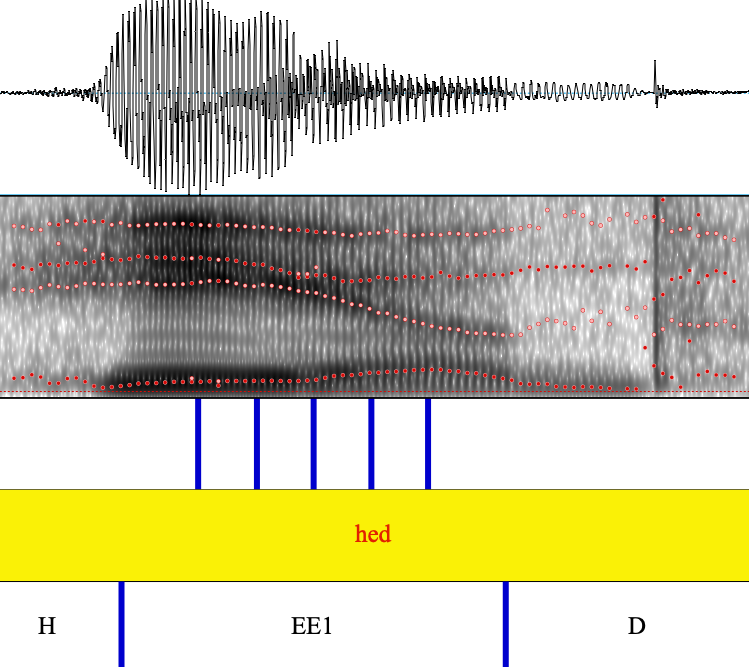
\includegraphics[width=0.4\linewidth]{spectrogram} 

}

\caption{Example of Praat textgrid with annotated segment boundaries and measurement points for the automatic extraction of F1-F3 formant frequencies.}\label{fig:spectrogram}
\end{figure}

In order to correct for measurement errors in the automatic extraction of cues, we estimated the joint multivariate distribution along all five extracted cues (F0, F1, F2, F3, and vowel duration) for each unique combination of vowel and talker. This approach allowed us to detect outliers relative to the joint distribution of the five cues for that vowel and talker. Points outside of the 0.5th to 99.5th quantile of the multivariate Gaussian distribution of each vowel were identified, checked for measurements errors, and corrected. For measurements of the first three formants, we first checked the segmentation boundaries in the Praat textgrid and then manually measured new formant values using visual approximation of time points and Praat's function \emph{Formant: Formant listing} or manually reading off the spectrogram. Segmentation boundaries were also checked for the identified vowel duration outliers. For measurements of F0, we extracted new estimated F0s across the vowel, after changing the pitch range settings. Given that there were still instances of pitch halving after measurement correction, in order to be conservative, we also checked all F0 values below the point of intersection between the two halves. The database available via OSF reports these corrected values (since the recordings and annotation grids are also available via OSF, other researchers can easily derive alternative measurements).\footnote{We note that outlier detection and correction was based on raw, rather than transformed/normalized, cue values. For the studies we report below, this potentially introduces a bias \emph{against} normalization. If anything, the present study is thus likely to under-estimate the effects of normalization.}

The procedure of adding written guides to \emph{hod} and \emph{hodd} to facilitate vowel identification was mostly successful, however not for all talkers. Some talkers corrected themselves after one trial, others failed to produce the intended vowel altogether. The SwehVd database contains columns for both the targeted vowel category, and the vowel category that the talker actually produced (as annotated by the first author).

For the vast majority of talkers, \emph{hädd} productions elicited the same vowel as \emph{hedd} (see Figure \ref{fig:hedd}). This confirms the common assumption that the short allophone to /e/ neutralizes with the short allophone to {[}\ipatext{ɛ}{]} in Central Swedish.



\begin{figure}

{\centering \includegraphics[width=0.3\linewidth]{SwehVd-article_files/figure-latex/hedd-1} 

}

\caption{The \emph{hedd} and \emph{hädd} words in the SwehVd vowel data in unnormalized F1-F2 space. Points show recordings of the \emph{hedd} and \emph{hädd} words ({[}\ipatext{ɛ}{]}) by the 23 female native talkers in the database, averaged across the five measurement points within each vowel segment. Word labels indicate word means across talkers. Since \emph{hädd} and \emph{hedd} resulted in the same allophone, we exclude \emph{hädd} from this and all other visualizations below. This facilitates comparison of, for example, densities across vowels (see diagonal of Figure \ref{fig:swe-vowels-all-cues}).}\label{fig:hedd}
\end{figure}

\hypertarget{sec:characterizing-swehvd}{%
\subsection*{Characterizing vowel productions in SwehVd}\label{sec:characterizing-swehvd}}
\addcontentsline{toc}{subsection}{Characterizing vowel productions in SwehVd}

Figure \ref{fig:swe-vowels} visualizes the vowel data from the SwehVd in F1-F2 space. The plot highlights the density of the Central Swedish vowel space, the categories are numerous and closely located. Category overlap is especially large among some of the high vowels (e.g., {[}\ipatext{iː}{]} \& {[}\ipatext{yː}{]}; {[}\ipatext{uː}{]}, {[}\ipatext{oː}{]} \& {[}\ipatext{ʊ}{]}). The contextually conditioned allophone {[}\ipatext{æ}{]}, almost completely overlaps with the long {[}\ipatext{ɛː}{]}, whereas the contextual allophones to {[}\ipatext{ø}{]} are more separated. Not all contextual allophones are articulated lower (higher F1) in relation to their phonemes (compare e.g., \protect\hyperlink{ref-riad2014}{Riad, 2014}). They are, however, all articulated further back (lower F2).

In line with Riad (\protect\hyperlink{ref-riad2014}{2014}, cf.~Table \ref{tab:swedish-vowels} above), the short vowels are overall more centralized and form a more condensed space, whereas the long vowels are more dispersed.\footnote{{[}\ipatext{ɪ}{]} and {[}\ipatext{ʏ}{]} are, however, more fronted than their long counterparts, which does not replicate previous descriptions of Central Swedish. We elaborate on this result in other ongoing work (\protect\hyperlink{ref-persson2023}{Persson, 2023}).} Differences in formant patterns between long and short vowels have been found to be smallest for the allophones to {[}\ipatext{ɛ}{]} and {[}\ipatext{ø}{]}, and largest for /u/ ({[}\ipatext{ʉː}{]} and {[}\ipatext{ɵ}{]}), and /a/ ({[}\ipatext{ɑː}{]} and {[}\ipatext{a}{]}) (e.g., \protect\hyperlink{ref-fant2001}{Fant, 2001}; \protect\hyperlink{ref-kuronen2000}{Kuronen, 2000}). This pattern does not entirely replicate here. We do see large differences in F1-F2 for the allophones to /u/ and /a/, but also substantial differences between {[}\ipatext{ɛ}{]} and {[}\ipatext{ɛː}{]}. Formant differences are apparent even for some category distinctions for which quantity has been found to be the primary cue (as shown in perceptual studies, see e.g., \protect\hyperlink{ref-behne1997}{Behne et al., 1997}; \protect\hyperlink{ref-haddingkoch1964}{Hadding-Koch and Abramson, 1964}), ({[}\ipatext{ɛː}{]} - {[}\ipatext{ɛ}{]}, {[}\ipatext{øː}{]} - {[}\ipatext{ø}{]}, {[}\ipatext{iː}{]} - {[}\ipatext{ɪ}{]}, and {[}\ipatext{oː}{]} - {[}\ipatext{ɔ}{]}).

Figure \ref{fig:swe-vowels-all-cues} visualizes the vowel data from the SwehVd database for all pairwise combinations of five cues: F0, F1, F2, F3 and vowel duration. As is to be expected, vowels differing in quality are most separated in the F1-F2 plot, indicating the two cues most important for vowel category distinction. However, the F1-F3 and F3-F2 plots both display less overlap between the high vowels {[}\ipatext{iː}{]}, {[}\ipatext{yː}{]} and {[}\ipatext{ʉː}{]}, comparing to when plotted along F1-F2. The increased separation of these categories along F3 in vowel production data could point to the importance of F3 for some category distinctions, as found in previous studies (see e.g., \protect\hyperlink{ref-fant1969}{Fant et al., 1969}; \protect\hyperlink{ref-fujimura1967}{Fujimura, 1967}; \protect\hyperlink{ref-kuronen2000}{Kuronen, 2000}, for {[}\ipatext{iː}{]} and {[}\ipatext{yː}{]} categorization).

Also as expected, duration is the primary cue that distinguishes vowel quantity: in the last column of Figure \ref{fig:swe-vowels-all-cues}, the short vowels cluster on the left, and the long vowels on the right. They are separable, but overlapping. Overall, the short vowels seem to display less variability in duration than the long vowels, a common pattern for measures with a lower bound. In addition to duration, F1-F3 can also carry information about vowels differing in quantity. This is evident, for example, for {[}\ipatext{iː}{]} vs.~{[}\ipatext{ɪ}{]}, {[}\ipatext{yː}{]} vs.~{[}\ipatext{ʏ}{]}, {[}\ipatext{ʉː}{]} vs.~{[}\ipatext{ɵ}{]}, {[}\ipatext{ɑː}{]} vs.~{[}\ipatext{a}{]}, {[}\ipatext{ɛː}{]} vs.~{[}\ipatext{ɛ}{]} in F1-F2 space, and for {[}\ipatext{iː}{]} vs.~{[}\ipatext{ɪ}{]}, {[}\ipatext{yː}{]} vs.~{[}\ipatext{ʏ}{]}, {[}\ipatext{ʉː}{]} vs.~{[}\ipatext{ɵ}{]} in F2-F3 space.

Finally, the densities along the diagonal of Figure \ref{fig:swe-vowels-all-cues} suggest that F0 carries the least information about vowel identity, exhibiting the least between-category separation, followed by F3. This, too, is not surprising: while some accounts use F0 to \emph{normalize} F1 and F2 (e.g., \protect\hyperlink{ref-miller1989c}{Miller, 1989}; \protect\hyperlink{ref-Syrdal1986}{Syrdal and Gopal, 1986}), F0 is not considered an important cue to vowel identity by itself (for demonstrations that F0 can, however, have strong \emph{in}direct effects on vowel categorization, see \protect\hyperlink{ref-barreda2012a}{Barreda and Nearey, 2012}; \protect\hyperlink{ref-barreda2020a}{Barreda, 2020}).





\begin{figure}

{\centering \includegraphics[width=0.7\linewidth]{SwehVd-article_files/figure-latex/swe-vowels-1} 

}

\caption{The SwehVd vowel data in unnormalized F1-F2 space. Points show recordings of each of the 21 Central Swedish vowels by the 23 female native talkers in the database, averaged across the five measurement points within each vowel segment. Vowel labels indicate category means across talkers. Long vowels are boldfaced. Vowels that mismatched intended label are excluded (1.23976\% of all recordings). Note that the F1 and F2 axes are reversed. We follow this convention whenever plotting vowels in the F1-F2 space.}\label{fig:swe-vowels}
\end{figure}

\begin{figure}
\includegraphics[width=1\linewidth]{SwehVd-article_files/figure-latex/swe-vowels-all-cues-1} \caption{The same data as in Figure \ref{fig:swe-vowels} but for all pairwise combinations of five cues: F0, F1, F2, F3, and vowel duration. The primary purpose of this figure is to provide an overview of the SwehVd data. Additionally, comparisons across the panels sheds light on which cues carry information about vowel quality and vowel quantity, respectively. Note that, unlike in Figure \ref{fig:swe-vowels}, axis directions are not reversed. \textbf{Panels on diagonal:} marginal cue densities of all five cues. \textbf{Lower off-diagonal panels:} each point corresponds to a recording, averaged across the five measurement points within each vowel segment. Vowel labels indicate category means across talkers. Long vowels are boldfaced. \textbf{Upper off-diagonal panels:} Same data as in the lower off-diagonal panels but showing bivariate Gaussian 95\% probability mass ellipses around category means. This makes it more obvious, for example, that long and short vowels are primarily distinguished by vowel duration (top right panel).}\label{fig:swe-vowels-all-cues}
\end{figure}

\hypertarget{sec:studyI}{%
\section*{Study 1: Comparing the effects of normalization accounts on between- vs.~within-category variability}\label{sec:studyI}}
\addcontentsline{toc}{section}{Study 1: Comparing the effects of normalization accounts on between- vs.~within-category variability}

In Study 1, we follow previous research on the effects of different normalization accounts on category variability, by evaluating how effectively different normalization accounts reduce the within-category variability of Central Swedish vowels. We visualize the vowel space under different normalization accounts, and assess the effects on vowel category variability by calculating a measure of category separability. To anticipate one take-home point of Study 1, the results highlight important shortcomings of separability indices in evaluating normalization accounts.

\begin{landscape}\begin{table}

\caption{\label{tab:norm-evaluation-variability}Previous studies comparing the effectiveness of normalization accounts in reducing within-category cue variability}
\centering
\fontsize{7}{9}\selectfont
\begin{tabular}[t]{>{\raggedright\arraybackslash}p{2cm}>{\raggedright\arraybackslash}p{2cm}>{\raggedright\arraybackslash}p{5.5cm}>{\raggedright\arraybackslash}p{6cm}>{\raggedright\arraybackslash}p{2.5cm}>{\raggedright\arraybackslash}p{2.5cm}}
\toprule
Language investigated & Article & Speech materials & Normalization accounts & Approach & Best two performing\\
\midrule
 & Barreda \& Nearey, 2018 & 120,000 simulated languages (of 5 or 9 vowels) modeled on Hillenbrand et al.'s (1995) data (98 female/male child/adult talkers * 12 vowels) & Nearey2, Lobanov, log-mean in linear regression framework & distance between means (Eucledian distance) & log-mean in linear regression framework (1), Nearey2 (2)\\
\cmidrule{2-6}
 & Clopper, 2009 & 2 female/male talkers from Ohio (1 token * 10 vowels) & Bladon et al.'s scale factor of 1 Bark (1994), Syrdal \& Gopal, Nordström \& Lindblom, Nearey1, Nearey2, Watt \& Fabricius, Gerstman, Lobanov, Miller & variance reduction (visual inspection) & Nearey, Watt \& Fabricius, Gerstman, Lobanov (no order)\\
\cmidrule{2-6}
 & Hindle, 1978 & Peterson \& Barney's (1952) database; 19 female/male talkers from Philadelphia + 60 telephone informants (minimum 3 tokens per category; analysis focus on /ay/) & Nearey2, Nordström-Lindblom, Sankoff-Shorrock-McKay & distance between means, variance reduction (regression) & Sankoff (1)\\
\cmidrule{2-6}
 & Kohn \& Farrington, 2012 & Longitudinal data from 10 female/male African American talkers from North Carolina (approx. 10 tokens * 10 vowels * 5 ages) & Lobanov, Gerstman, Nearey1, Nordström \& Lindblom, Syrdal \& Gopal/Thomas, Watt \& Fabricius & variance reduction (regression) & Lobanov (1), Gerstman, Watt \& Fabricius (2)\\
\cmidrule{2-6}
\multirow{-5}{2cm}{\raggedright\arraybackslash US English} & Labov, 2010 & Peterson \& Barney's (1952) database; Philadelphia/Linguistic Change and Variation project (120 female/male talkers, stratified for age, sociolinguistic factors) & Nearey2, Nordström-Lindblom, Sankoff-Shorrock-McKay & distance between means (F-statistics) & Sankoff (1), Nearey2 (2)\\
\cmidrule{1-6}
US English, Norwegian, Swedish, German, Danish, Dutch & Disner, 1980 & Differing number of tokens, vowels, and phonetic contexts across the six languages & Gerstman, Lobanov, Nearey2, Harshman's PARAFAC model & variance reduction (visual inspection) & Nearey2 (1), Lobanov (2)\\
\cmidrule{1-6}
 & Fabricius, Watt \& Johnson, 2009 & 20 old/young female/male talkers of Received pronunciation (11 vowels); 6 old/young female/male talkers of Aberdeen English (8 vowels in different phonetic contexts) & Watt \& Fabricius, Lobanov, Nearey1 &  & Lobanov (1), Watt \& Fabricius (2)\\
\cmidrule{2-4}
\cmidrule{6-6}
\multirow{-2}{2cm}{\raggedright\arraybackslash UK English} & Flynn \& Foulkes, 2011 & 20 old/young female/male Nottingham talkers (mean 180 recordings per talker; categories not reported) & log-transformation (base 10), log-transformation (natural), Mel, ERB, Bark (*2 gender-specific versions), Syrdal \& Gopal, Nordström (*2 gender-specific versions), LCE, Gerstman, Lobanov, Watt \& Fabricius (* 4 versions), lettER, Nearey (*4 versions) & \multirow{-2}{2.5cm}{\raggedright\arraybackslash variance reduction (SCV in talker-means)} & Gerstman (1), LCE (2)\\
\cmidrule{1-6}
Russian & Lobanov, 1971 & 5 female/male talkers (9 vowels in different phonetic contexts) & linear compression or expansion (Fant, 1960), Gerstman, Lobanov & distance between means & Lobanov (1), Gerstman (2)\\
\bottomrule
\end{tabular}
\end{table}
\end{landscape}

Table \ref{tab:norm-evaluation-variability} lists previous studies that have compared normalization accounts in terms of their effectiveness in reducing inter-talker variability. These studies varied in the specific metrics they employed to assess the effects of normalization, the languages they studied, and the conclusions they arrived at. Two generalizations emerge from Table \ref{tab:norm-evaluation-variability}. First, transformation to a perceptual scale alone does not seem to be sufficient to reduce inter-talker variability (see also \protect\hyperlink{ref-adank2004}{Adank et al., 2004}; \protect\hyperlink{ref-carpenter1993}{Carpenter and Govindarajan, 1993}; \protect\hyperlink{ref-clopper2009}{Clopper, 2009}; \protect\hyperlink{ref-escudero2007}{Escudero and Bion, 2007}; \protect\hyperlink{ref-Flynn2011}{Flynn and Foulkes, 2011}; \protect\hyperlink{ref-kohn2012a}{Kohn and Farrington, 2012}). Second, normalization accounts that include centering and/or standardizing seem to perform best in reducing inter-talker variability (see e.g. \protect\hyperlink{ref-barreda2018a}{Barreda and Nearey, 2018}; \protect\hyperlink{ref-disner1980}{Disner, 1980}; \protect\hyperlink{ref-fabricius2009}{Fabricius et al., 2009}; \protect\hyperlink{ref-kohn2012a}{Kohn and Farrington, 2012}; \protect\hyperlink{ref-labov2010}{Labov, 2010}; \protect\hyperlink{ref-lobanov1971}{Lobanov, 1971}). When Lobanov and Gerstman normalization---both involving standardizing---were included in a study, they often rank among the top two performing accounts. Of note, Nearey normalization (\protect\hyperlink{ref-nearey1978}{Nearey, 1978}) seems to perform well even though it does not involve the computationally more complex operation of standardizing. This suggests that simple centering of formants relative to the talker's mean \emph{might} be sufficient to achieve significant variance reduction (but see \protect\hyperlink{ref-disner1980}{Disner, 1980} for Swedish, which is revisited in this study).

\hypertarget{sec:methodsI}{%
\subsection*{Methods}\label{sec:methodsI}}
\addcontentsline{toc}{subsection}{Methods}

\hypertarget{sec:speechMaterialsI}{%
\subsubsection*{Speech materials}\label{sec:speechMaterialsI}}
\addcontentsline{toc}{subsubsection}{Speech materials}

We use the SwehVd database with some exclusions. Since we are interested in assessing the effects of normalization, we excluded any productions on which the talker did not produce the targeted vowel. We then excluded all talkers (N = 7) with fewer than 5 remaining recordings for at least one of the vowels. Five of these talkers rarely ever produced the targeted {[}\ipatext{ʊ}{]} vowel despite our recording instructions (see \protect\hyperlink{sec:cue-extraction}{Extraction of phonetic cues}). Instead, they often mispronounced the vowel. This left data from 16 female native talkers, with on average 797 (se= 2.5) tokens per vowel (range = 765 to 815), for a total of 16730 observations.

Since our goal is to obtain a reliable estimate of the formant values during the steady state of the vowel, we use only the three formant measurements extracted from the middle of the vowel (at 35\%, 50\%, and 65\% into the vowel).\footnote{While this is the approach most commonly employed in the literature, it has the potential downside that co-articulation might affect formant values at the measurement points differently for long and short vowels (since the long and short vowels differ in overall duration). An alternative approach would be to extract formants at fixed durations (e.g., 30 ms) after the vowel onset and before the vowel offset. Since the findings we present below do not indicate any systematic differences in the performance of normalization accounts between long and short vowels, we do not consider this issue further here.}

We also exclude all \emph{hädd} productions, as they elicited the same vowel as \emph{hedd} (see \protect\hyperlink{sec:cue-extraction}{Extraction of phonetic cues}). This way, we have about equally many tokens from all vowels, simplifying the cross-validation procedure presented below and facilitating visual comparisons across vowels in our figures.

\hypertarget{sec:cues}{%
\subsubsection*{Cues included in the normalization}\label{sec:cues}}
\addcontentsline{toc}{subsubsection}{Cues included in the normalization}

We compare the effect of different normalization accounts on the variability of Central Swedish vowels under three different assumptions about the relevant cues. The first comparison follows most previous research and focuses on the two primary cues to vowel perception, F1 and F2. The second comparison considers F3 in addition to F1 and F2, following Adank et al. (\protect\hyperlink{ref-adank2004}{2004}), Barreda and Nearey (\protect\hyperlink{ref-barreda2018a}{2018}), Nearey (\protect\hyperlink{ref-nearey1989}{1989}) and Syrdal (\protect\hyperlink{ref-syrda1985}{1985}).\footnote{Some of these studies additionally included F0 (\protect\hyperlink{ref-adank2004}{Adank et al., 2004}; \protect\hyperlink{ref-nearey1989}{Nearey, 1989}; \protect\hyperlink{ref-syrda1985}{Syrdal, 1985}). However, since F0 is a cue that can display substantial cross-talker variability without directly contributing much information to vowel categorization (recall Figure \ref{fig:swe-vowels-all-cues}), its inclusion can reduce the informativeness of the separability index. We therefore decided to add only F3 to F1-F2 in the second evaluation.} Finally, the third comparison includes F0 and duration in addition to F1-F3. Since Syrdal and Gopal (\protect\hyperlink{ref-Syrdal1986}{1986})'s bark-difference model only considers normalization along two dimensions---height, implemented as F1-F0, and backness, implemented as F2-F1---this account will only be included in the first comparison. Furthermore, given that C-CuRE is the only account that applies to any type of cue, we will consider duration as centered to each talker's mean (for the C-CuRE accounts), or as raw input (in ms; for all other accounts). To our knowledge, duration has not been considered in previous studies on normalization, presumably because the present study is the first to evaluate normalization accounts against a vowel system with a systematic quantity distinction (long vs.~short vowels). We evaluate the effect on variability both separately for long and short vowels, and on all 21 vowels together.

\hypertarget{sec:separabilityIndex}{%
\subsubsection*{Separability index}\label{sec:separabilityIndex}}
\addcontentsline{toc}{subsubsection}{Separability index}

Previous studies have used different measures to assess the relative success of a normalization procedure in reducing inter-talker variability (see Table \ref{tab:norm-evaluation-variability} and \protect\hyperlink{ref-nearey1989}{Nearey, 1989} for an overview on classification accounts). This includes assessing the reduction in variance or distance between means by visual inspection (e.g., \protect\hyperlink{ref-clopper2009}{Clopper, 2009}; \protect\hyperlink{ref-disner1980}{Disner, 1980}; \protect\hyperlink{ref-hindle1978}{Hindle, 1978}), or by calculating the reduction in within-category variance across talkers (e.g., \protect\hyperlink{ref-disner1980}{Disner, 1980}; \protect\hyperlink{ref-fabricius2009}{Fabricius et al., 2009}; \protect\hyperlink{ref-Flynn2011}{Flynn and Foulkes, 2011}; \protect\hyperlink{ref-hindle1978}{Hindle, 1978}), or comparing the degree of separation between category means for unnormalized and normalized data, i.e., an F-ratio (e.g., \protect\hyperlink{ref-labov2010}{Labov, 2010}).

We will assess how distinguishable vowels become under different normalization accounts by calculating a separability index, as described in Equation \eqref{eq:separability-index}. Following some previous studies (e.g., \protect\hyperlink{ref-labov2010}{Labov, 2010}), this separability index is essentially an F statistics, where the F statistics is the ratio of the within- and between-category variances:

\begin{equation}\label{eq:separability-index}
\begin{split}
 separability\ index &= \frac{between\ category\ MS}{within\ category\ MS}\\
 &= \frac{\sum\limits_{c=1,\ldots,K}(N_{c}-1)}{K-1}\frac{\sum\limits_{c=1,\ldots,K}(\bar{x}_{c}-\bar{x})^{2}}{\sum\limits_{c=1,\ldots,K} \sum\limits_{i=1,\ldots,N_{c}}(x_{i,c}-\bar{x}_{c})^{2}}
\end{split}
\end{equation}

where \(K\) is the number of categories, \(N_c\) is the number of observations for category \(c\), \(x_{i,c}\) is the cue vector (for all cues considered in the calculation of the separability index) for observation \(i\) of category \(c\), \(\bar{x}_c\) is the cue mean vector for category \(c\), and \(\bar{x}\) is the overall cue mean vector. We calculated this separability index separately for each combination of normalization account, cues, and training-test fold, as described next.

\hypertarget{sec:folds}{%
\subsubsection*{Guarding against over-fitting: cross-validation}\label{sec:folds}}
\addcontentsline{toc}{subsubsection}{Guarding against over-fitting: cross-validation}

As shown in Table \ref{tab:norm-accounts}, many of the normalization accounts involve parameters that are set based on the data (e.g., \protect\hyperlink{ref-gerstman1968}{Gerstman, 1968}; \protect\hyperlink{ref-lobanov1971}{Lobanov, 1971}; \protect\hyperlink{ref-mcmurray-jongman2011}{McMurray and Jongman, 2011}; \protect\hyperlink{ref-miller1989c}{Miller, 1989}; \protect\hyperlink{ref-nearey1978}{Nearey, 1978}). This raises the question of how much these parameters can be affected by outliers, or other issues such as over-fitting to the sample. Unlike previous work, we thus use 5-fold cross-validation to obtain 5 separate estimates of the separability index for each combination of normalization procedure and cues. Specifically, we randomly split the data for each unique combination of talker and vowel into 5 even parts (folds). On each of the five folds, we then fit the normalization parameters based on four of the folds (the training data) and evaluated the effects of the normalization on the fifth fold (the test data). This resulted in five separability indices for each combination of normalization procedure and cues.

\hypertarget{sec:resultsI}{%
\subsection*{Results}\label{sec:resultsI}}
\addcontentsline{toc}{subsection}{Results}

\hypertarget{sec:normVowelSpace}{%
\subsubsection*{Visualizing the distribution of vowel productions}\label{sec:normVowelSpace}}
\addcontentsline{toc}{subsubsection}{Visualizing the distribution of vowel productions}

Figures \ref{fig:swe-vowels-normalized-long} and \ref{fig:swe-vowels-normalized-short} visualize the Central Swedish vowels in the test data, after applying the 15 different scale-transformations and normalization accounts for a visual inspection. For this purpose, we focus on F1 and F2 only. The SI includes similar pairwise correlation plots of all cues for all different normalization accounts we compare (see \protect\hyperlink{sec:correlation-matrices}{SI, Correlation matrices}).

Visual inspection suggests a few initial observations. The most striking difference is perhaps between intrinsic normalization accounts (\protect\hyperlink{ref-Syrdal1986}{Syrdal and Gopal, 1986}; \protect\hyperlink{ref-miller1989c}{Miller, 1989}) and all other approaches, though it is not immediately visually obvious which type of approach achieves better separability. Second, transforming the vowels to a different perceptual scale does not seem to affect the vowel distributions much, besides a minor decrease in category variance for some of the vowels. Some transformations bring the vowel categories closer together, towards the center of the vowel space, e.g., ERB and semitones. Third, centering formants by subtracting each talkers' mean (\protect\hyperlink{ref-mcmurray-jongman2011}{McMurray and Jongman, 2011}; \protect\hyperlink{ref-nearey1978}{Nearey, 1978}) reduces some of the category variance, and as a result, increases the category separability. Transforming the vowel data into different scales prior to centering also seems to further improve separability (compare e.g., C-CuRE (Hz) and C-CuRE (semitones)). Overall, the top two performing accounts across the long and short vowels appear to be Lobanov (\protect\hyperlink{ref-lobanov1971}{1971}) and Nearey (\protect\hyperlink{ref-nearey1978}{1978}). However, even for the best performing normalization accounts, there is still considerable category overlap. This involves some of the high long vowels, and some of the mid-center short vowels. This highlights the need to more systematically quantify the effects of normalization, as we do next for category separability and then in more depth in Study 2.





\begin{landscape}

\begin{figure}

{\centering \includegraphics[width=0.9\linewidth]{SwehVd-article_files/figure-latex/swe-vowels-normalized-long-1} 

}

\caption{The 11 long vowels of Central Swedish when F1 and F2 are left unnormalized or transformed into a perceptual scales (\textbf{grey}), intrinsically normalized (\textbf{yellow}), or extrinsically normalized through centering (\textbf{blue}) or standardizing (\textbf{purple}). Each point corresponds to one recording, averaged across the five measurement points within each vowel segment. Each panel combines the data from all five test folds.}\label{fig:swe-vowels-normalized-long}
\end{figure}

\end{landscape}

\begin{landscape}
\begin{figure}

{\centering \includegraphics[width=0.9\linewidth]{SwehVd-article_files/figure-latex/swe-vowels-normalized-short-1} 

}

\caption{The 10 short vowels of Central Swedish when F1 and F2 are left unnormalized or transformed into a perceptual scales (\textbf{grey}), intrinsically normalized (\textbf{yellow}), or extrinsically normalized through centering (\textbf{blue}) or standardizing (\textbf{purple}). Each point corresponds to one recording, averaged across the five measurement points within each vowel segment. Each panel combines the data from all five test folds.}\label{fig:swe-vowels-normalized-short}
\end{figure}

\end{landscape}

\hypertarget{sec:normVariability}{%
\subsubsection*{The effect of normalization accounts on the variability of Central Swedish vowels}\label{sec:normVariability}}
\addcontentsline{toc}{subsubsection}{The effect of normalization accounts on the variability of Central Swedish vowels}

In order to assess the effects of normalization accounts on category separability, we calculate a separability index under different assumptions about the relevant cues and the size of the vowel space (the long and short vowels separately, or the entire space). Before we evaluate how category separability is affected by normalization in F1-F2, F1-F3, and F0-F3 and duration space, we look at how the normalization accounts affect the separability of vowels along each cue separately (Figure \ref{fig:separability-by-cue}). As we show below, this is helpful in understanding the subsequently presented results for combinations of cues.



\begin{figure}

{\centering \includegraphics[width=1\linewidth]{SwehVd-article_files/figure-latex/separability-by-cue-1} 

}

\caption{Separability indices by normalization accounts for long vowels, short vowels, and long and short vowels together (columns), shown for each of the five cues considered in this study (rows). Labels indicate mean across the five test folds. Intervals show average bootstrapped 95\% confidence intervals across the test folds. Note that the ranges of the y-axes varies across plots.}\label{fig:separability-by-cue}
\end{figure}

For F1 (first row of Figure \ref{fig:separability-by-cue}), we see a clear advantage for centering (in blue) and standardizing (in purple) compared to transformations (in grey) and intrinsic accounts (in yellow). In particular Lobanov normalization seems to maximize category separability along F1, at least for the long vowels and all vowels together. Notably, the accounts pattern differently along F2 (second row of Figure \ref{fig:separability-by-cue}). Overall, differences between accounts are much smaller along F2, and the clear advantage of centering and standardizing accounts along F1 does not extend to F2.

An altogether different picture is observed for F3. Compared to F1 and F2, the intrinsic account (Miller) performs substantially better in separating categories along F3, while all other accounts perform poorly. This result is surprising: one of the downsides of intrinsic approaches that has been noted in previous work is their sensitivity to measurement error (\protect\hyperlink{ref-thomas2007}{Thomas and Kendall, 2007}). This sensitivity is caused by the fact that intrinsic accounts use a single measurement for normalization, rather than the less noisy estimates resulting from aggregating across segments that are used in extrinsic accounts. Since the third formant is often described as more difficult to reliably estimate than other formants (leading to more measurement error), F3 would be expected to be particularly affected by this weakness of intrinsic accounts.

Yet, further visualization in Figure \ref{fig:F3-densities} confirms that F3 indeed separates categories particularly well when intrinsic normalization is applied. Compared to other accounts, Miller (\protect\hyperlink{ref-miller1989c}{1989}) seems to be particularly successful in separating vowels that differ in lip rounding. For example, Miller (\protect\hyperlink{ref-miller1989c}{1989}) separates two clusters among the high and mid-high vowels, one consisting of the back vowels \ipatext{[oː]} and \ipatext{[uː]}, and the other one of the front \ipatext{[iː]}, and rounded \ipatext{[yː]} and \ipatext{[ʉː]}. One possible explanation for this result is that intrinsic normalization is indeed particularly effective for F3, and that our correction of measurement errors---equally applied to all formants---effectively reduced the issue with F3 measurement errors (presumably the human brain, too, can do better than an uncorrected Praat algorithm without error correction). As we show below, this result for F3 carries over to any combination of cues that includes F3. It is, however, an artifact of using category separability to assess the effectiveness of normalization, as we show in Study 2. We elaborate on this issue in the discussion of Study 1.

Returning to Figure \ref{fig:separability-by-cue}, normalization does not increase category separability for F0. This is expected given that F0 is known to affect vowel separability primarily through its indirect influence on the interpretation of other formants (e.g., \protect\hyperlink{ref-barreda2012a}{Barreda and Nearey, 2012}; \protect\hyperlink{ref-barreda2020a}{Barreda, 2020}). Finally, for duration all of the C-CuRE accounts group together against the remaining accounts. This, too, is expected since all other accounts are formant-specific and thus do not normalize duration. In summary, the five cues contribute to category separability in different ways, and this is reflected in varying effectiveness of different normalization accounts. We also note that the best performing normalization account for any combination of cues and vowel qualities is typically never significantly better than the next best performing model (the 95\% confidence intervals of the best model overlap with the mean of the next best model). In fact, for many combinations of cues and vowel qualities, many of the models perform similarly.



\begin{figure}

{\centering \includegraphics[width=0.95\linewidth]{SwehVd-article_files/figure-latex/F3-densities-1} 

}

\caption{Category densities along F3 illustrates the effectiveness of vowel-intrinsic normalization for this cue. Here shown for Miller, compared to vowel-extrinsic accounts that center and/or standardize cues. For reference, densities in the absence of normalization are also shown.}\label{fig:F3-densities}
\end{figure}

Next, we summarize how normalization affects category separability when combinations of the fives cues are considered. Figure \ref{fig:separability} shows the separability index for the different normalization accounts for three different combinations of cues. For the first row of Figure \ref{fig:separability}, we followed most previous research in assessing category separability for the combination of F1 and F2 (e.g., \protect\hyperlink{ref-disner1980}{Disner, 1980}; \protect\hyperlink{ref-fabricius2009}{Fabricius et al., 2009}; \protect\hyperlink{ref-Flynn2011}{Flynn and Foulkes, 2011}; \protect\hyperlink{ref-hindle1978}{Hindle, 1978}; \protect\hyperlink{ref-labov2010}{Labov, 2010}). Accounts that center against the talker's overall formant mean (in blue) are among the best performing normalization accounts. No matter the assumed perceptual scale, centering always improves category separability. Standardizing accounts (in purple), primarily Lobanov (\protect\hyperlink{ref-lobanov1971}{1971}), also perform well at separating categories, more so for the long vowels. However, scale transformations (in grey), and intrinsic accounts (in yellow), do not improve category separability compared to unnormalized Hz, at least not when assessed on the long vowels or the entire vowel space.

The remaining rows of Figure \ref{fig:separability} compare normalization accounts when F3 (second row) or F0, F3, and duration are included (third row). Overall, the category separability is now lower, a result of how the accounts affect category separability along the cues added (see Figure \ref{fig:separability-by-cue}). The most drastic change in performance concerns the intrinsic Miller (\protect\hyperlink{ref-miller1989c}{1989}) and the standardizing accounts. When including F3, Miller (\protect\hyperlink{ref-miller1989c}{1989}) performs as well or better, in absolute numbers, as when evaluated on only the combination of F1 and F2, thereby increasing its performance relative to other accounts. This increase in performance might be particularly pronounced for languages like Swedish, where F3 carries important information about lip rounding and thus vowel identity. In contrast, performance of standardizing accounts drops substantially if F3 or any other cue besides F1 and F2 is included.\footnote{We confirmed this by conducting additional comparisons using only F1, F2 and F0, or only F1, F2 and duration. For both of these comparisons too, we found that standardizing accounts perform poorly.} This mirrors what was found when assessing category separability separately for each cue (Figure \ref{fig:separability-by-cue}).

Finally, looking across all three rows, category separability is consistently higher for short than long vowels. The same pattern is evident for each cue separately in Figure \ref{fig:separability-by-cue}. This result might initially be puzzling, given that previous descriptions of Central Swedish vowel inventories characterize the inventory of short vowels as being more centralized and more densely clustered (e.g., \protect\hyperlink{ref-kuronen2000}{Kuronen, 2000}; \protect\hyperlink{ref-riad2014}{Riad, 2014}). Indeed, this claim seems to hold for SwehVd---compare Figures \ref{fig:swe-vowels-normalized-long} and \ref{fig:swe-vowels-normalized-short}. However, the short vowels exhibit less category variability and less category overlap, making them overall more separable.



\begin{figure}

{\centering \includegraphics[width=1\linewidth]{SwehVd-article_files/figure-latex/separability-1} 

}

\caption{Separability indices by normalization accounts for long vowels, short vowels, and both long and short vowels together (columns) shown for three different combinations of cues (rows). Labels indicate mean across the five test folds. Intervals show average bootstrapped 95\% confidence intervals across the test folds. Note that the ranges of the y-axes varies across plots.}\label{fig:separability}
\end{figure}

\hypertarget{sec:studyI-discussion}{%
\subsection*{Discussion}\label{sec:studyI-discussion}}
\addcontentsline{toc}{subsection}{Discussion}

When only F1 and F2 are considered, as in most previous work on vowel normalization, we find that extrinsic centering and standardizing accounts achieve the best category separability. Within these two types of accounts, there is considerable variability. For example, among the intrinsic accounts, Miller performs worse than Syrdal \& Gopal, among the extrinsic accounts, versions of C-CuRE seem to consistently perform best. It is also worth noting, however, that there is never a single account that performs significantly better than all other normalizations. This points to the inherent similarities across normalization accounts, and perhaps limitations of the approach taken here (and in some previous work). We return to this point in the general discussion. Regardless of these caveats, the findings for F1 and F2 of Study I, revise the results of Disner (\protect\hyperlink{ref-disner1980}{1980}) for Swedish, and instead replicates previous findings for the other Germanic languages in Disner's sample as well as the majority of previous studies on other languages (e.g., \protect\hyperlink{ref-fabricius2009}{Fabricius et al., 2009}; \protect\hyperlink{ref-Flynn2011}{Flynn and Foulkes, 2011}; \protect\hyperlink{ref-labov2010}{Labov, 2010}).

However, when F3 is considered along with F1 and F2, this result does no longer hold. Key to understanding this result and what it says about the suitability of category separability as a measure of normalization accounts is Figure \ref{fig:separability-by-cue}: while extrinsic normalization performs better than other approaches for F1 and F2, the absolute differences in performance are small compared to the advantage of the intrinsic account observed for F3. Combined with a seemingly innocuous aspect of the separability index in Equation \eqref{eq:separability-index}, this allows separability along F3 to dominate separability along the other cue dimensions. Our separability index takes the \emph{sum} of (squared) distances along each cue dimension, essentially assuming that the effect of all cues is simply a sum of each cue's effect considered separately. This means that the separability index cannot capture the \emph{joint} effect of cues---whether, for example, one cue effectively separates one set of categories and another cue separates another set of categories, rather than both cues separating the same categories. The separability index thus cannot recognize, for example, that F1 and F2 capture largely complementary aspects of the vowel inventory (as evident in, for example, Figures \ref{fig:swe-vowels-normalized-long} and \ref{fig:swe-vowels-normalized-short}).

This is not the only deficiency of the separability index or similar measures of category variability. The use of \emph{squared} distances means that even a small number of observations located far away from the category mean can disproportionally affect the index. Consider, for example, the F3 densities in Figure \ref{fig:F3-densities}. For non-intrinsic normalizations, some categories have low but non-zero densities far away from the mode. Because of the use of squared distances, this results in low category separability for these normalization accounts despite the fact that observations with such cue values are rare and thus not expected to have a large effect on the \emph{average} perceptual separability of vowels. For the same reason (the use of squared distances), category separability can be high even if a cue separates only a small subset of categories (as is the case for F3), compared to another cue that more gradiently separates \emph{all} categories (as is the case for F1 and F2; see Figure \ref{fig:swe-vowels-all-cues}).

Finally, measures like the separability index suffer from a conceptual issue: the goal of speech perception is presumably not to reduce cue variability around the category mean but rather to increase the probability of correct recognition (of both linguistic and social information, where we focus on the former here). These two goals are not the same (see also discussion in \protect\hyperlink{ref-barreda2020a}{Barreda, 2020}). In sum, indices of variability and category separability like that in Equation \eqref{eq:separability-index} fail to adequately assess the expected consequences of normalization for perception, which is the primary interest of this study. Study 2 addresses this issue.

\hypertarget{sec:studyII}{%
\section*{Study 2: Comparing the expected effects of normalization on perception}\label{sec:studyII}}
\addcontentsline{toc}{section}{Study 2: Comparing the expected effects of normalization on perception}

Study 2 takes a more direct approach to evaluating the expected effects of normalization for the perception of vowels. Specifically, we use a general model of speech perception, Bayesian ideal observers (e.g., \protect\hyperlink{ref-clayards2008}{Clayards et al., 2008}; \protect\hyperlink{ref-nearey1986a}{Nearey and Hogan, 1986}; \protect\hyperlink{ref-norris-mcqueen2008}{Norris and McQueen, 2008}), to predict the vowel identities in the SwehVd database under different normalization accounts. We then compare normalization accounts based on the recognition accuracy that they achieve when the (un)normalized cues are fed into the otherwise identical categorization model. We evaluate the same normalization accounts as those investigated in Study 1. And, as in Study 1, we repeat this comparisons for different combinations of cues, and while categorizing just long vowels, just short vowels, or both long and short vowels together.

\begin{landscape}\begin{table}

\caption{\label{tab:norm-evaluation-percep}Previous studies comparing normalization accounts in terms of their predicted consequences for perception}
\centering
\fontsize{7}{9}\selectfont
\begin{tabular}[t]{>{\raggedright\arraybackslash}p{2cm}>{\raggedright\arraybackslash}p{2cm}>{\raggedright\arraybackslash}p{5.5cm}>{\raggedright\arraybackslash}p{5.5cm}>{\raggedright\arraybackslash}p{2cm}>{\raggedright\arraybackslash}p{2cm}>{\raggedright\arraybackslash}p{1.5cm}}
\toprule
Language(s) investigated & Article & Speech materials & Normalization accounts & Approach & Accuracy assessed & Best two performing\\
\midrule
 & Barreda, 2021 & synthesized stimuli representing 6 talker types (based on data from 30 female/male talkers of California English (15 tokens * 11 vowels)) & Nearey2, Watt \& Fabricius, Lobanov & regression & against perceived category & Nearey2 (1), Watt \& Fabricius (2)\\
\cmidrule{2-7}
 & Carpenter \& Govindarajan, 1993 & Peterson \& Barney's (1952) database, 75 female/male child/adult talkers (2 tokens * 10 vowels) & Bark, Mel, ERB, 2 log-transformations, Syrdal \& Gopal, Miller, Nearey1, Nearey2, Gerstman, linear transformation (Watrous, 1993) & fuzzy ARTMAP, K-nearest neighbour & & linear transformation (1), Nearey1 (2)\\
\cmidrule{2-5}
\cmidrule{7-7}
 & Cole, Linebaugh, Munson \& McMurray, 2010 & 10 female/male talkers (3 tokens * 2 target vowels * 4 context vowels * 6 consonants) & C-CuRE & regression &  & C-CuRE (1)\\
\cmidrule{2-5}
\cmidrule{7-7}
 & Johnson \& Sjerps, 2021 & Peterson \& Barney's (1952) database, 75 female/male child/adult talkers (2 tokens * 10 vowels); Hillenbrand et al.'s (1995) database, 138 female/male child/adult talkers (1-3 tokens * 12 vowels) & Mean $\lambda$, F3 anchor, F1 anchor, Mean F* anchor (Sussman, 1986), Nordström, VTLN (Lammert \& Narayanan, 2015), Nearey2, Gerstman, VTLN ($\Delta$F), Nearey1, Watt \& Fabricius, Lobanov, Miller, Syrdal \& Gopal & support vector machine classification models &  & Lobanov (1), Watt \& Fabricius (2)\\
\cmidrule{2-5}
\cmidrule{7-7}
 & McMurray, Cole \& Munson, 2011 & Cole et al. (2010) database, 10 female/male talkers (1 token * 2 target vowels * 4 context vowels * 6 consonants) &  &  & \multirow{-12}{2cm}{\raggedright\arraybackslash against intended category} & \\
\cmidrule{2-3}
\cmidrule{6-6}
 & McMurray \& Jongman, 2016 & Jongman et al. (2000) database, 10 female/male talkers (1 token * 4 vowels * 8 fricatives) & \multirow{-2}{5cm}{\raggedright\arraybackslash C-CuRE} & \multirow{-2}{2cm}{\raggedright\arraybackslash regression} & & \multirow{-2}{2cm}{\raggedright\arraybackslash C-CuRE (1)}\\
\cmidrule{2-5}
\cmidrule{7-7}
 & Nearey, 1989 & synthesized stimuli of male child/adult talker (based on male talker data from Fant, 1973, and Peterson \& Barney, 1952) & intrinsic normalization, extrinsic normalization & response patterns (F-ratio) & & extrinsic effects (1), intrinsic effects (2)\\
\cmidrule{2-5}
\cmidrule{7-7}
 & Richter, Feldman, Salgado \& Jansen, 2017 & models based on Clopper \& Pisoni's (2006) NSP vowel corpus, 60 female/male talkers, 6 varieties (5 tokens * 10 vowels); perceptual data from Feldman et al., 2009 (synthesized stimuli of male talker) & Vocal Tract Length Normalization (VTLN), Lobanov & discrimination model likelihoods & \multirow{-6}{2cm}{\raggedright\arraybackslash against perceived category} & VTLN (1), Lobanov (2)\\
\cmidrule{2-7}
\multirow{-26}{2cm}{\raggedright\arraybackslash US English} & Syrdal, 1985 & Peterson \& Barney's (1952) database, 75 female/male child/adult talkers (2 tokens * 10 vowels) & log-transformation, Bark, Syrdal's bark-difference model, Miller (2 accounts), Nearey1, Nearey2, Gerstman & linear discriminant analysis &  & Nearey1 (1), Nearey2 (2)\\
\cmidrule{1-5}
\cmidrule{7-7}
Brazilian Portuguese \& US English & Escudero \& Hoffman Bion, 2007 & models trained on 400,000 F1-F2 combinations generated on recordings of 8 female/male talkers (20 tokens * 7 vowels and 15 tokens * 11 vowels) & Nearey1, Lobanov, Gerstman & constraint rankings &  & \\
\cmidrule{1-5}
Dutch & Adank, Smits \& van Hout, 2004 & 160 female/male talkers, 8 varieties (2 tokens * 9 vowels) & log-transformation, Bark, Mel, ERB, Syrdal \& Gopal, Lobanov, Nearey1, Nearey2\tablefootnote{Barreda \& Nearey (2018) identify a mistake in the implementation of the Nearey2 account in Adank et al. (2004), so that the relative performance of Nearey2 reported by Adank and colleagues should be interpreted with caution.}, Gerstman, Nordström, Miller & linear discriminant analysis & \multirow{-8}{2cm}{\raggedright\arraybackslash against intended category} & \multirow{-2}{2cm}{\raggedright\arraybackslash Lobanov (1), Nearey1 (2)}\\
\bottomrule
\end{tabular}
\end{table}
\end{landscape}

Table \ref{tab:norm-evaluation-percep} lists previous studies that have compared normalization accounts in terms of their expected consequences for perception. While some previous studies have evaluated normalization accounts against listeners' responses in perception experiments (\protect\hyperlink{ref-barreda2021}{Barreda, 2021}; \protect\hyperlink{ref-mcmurray-jongman2016}{McMurray and Jongman, 2016}; \protect\hyperlink{ref-nearey1989}{Nearey, 1989}; \protect\hyperlink{ref-richter2017}{Richter et al., 2017}), the majority of previous work has evaluated accounts against the category intended by the talker---i.e., against production data. Here, we follow this majority (though we plan to conduct perception studies on Central Swedish in the future).

Across languages and approaches, the studies in Table \ref{tab:norm-evaluation-percep} yield similar results as those summarized in Table \ref{tab:norm-evaluation-variability} for category separability. Normalization improves recognition accuracy compared to unnormalized cues. Perceptual transformations perform worse than intrinsic or extrinsic normalization at predicting perception from production data. Furthermore, the same normalization accounts that have been found to be most successful at reducing inter-talker variability (e.g., \protect\hyperlink{ref-lobanov1971}{Lobanov, 1971}; \protect\hyperlink{ref-nearey1978}{Nearey, 1978}) are also often found to achieve higher recognition accuracy (e.g., \protect\hyperlink{ref-adank2004}{Adank et al., 2004}; \protect\hyperlink{ref-escudero2007}{Escudero and Bion, 2007}; \protect\hyperlink{ref-johnson-sjerps2021}{Johnson and Sjerps, 2021}; \protect\hyperlink{ref-syrda1985}{Syrdal, 1985}). Despite these overall similarities in results, it is important to keep in mind that the two approaches---category separability and models of perception---do not \emph{have} to yield the same results. In the present study, we go beyond previous work by modeling perception of both vowel quality and vowel quantity over a particularly dense vowel space, and by considering additional cues.

As also shown in Table \ref{tab:norm-evaluation-percep}, previous work has employed a number of model types to compare the expected effects of normalization on perception, ranging from models based on phonological theory (e.g., optimality theory, \protect\hyperlink{ref-escudero2007}{Escudero and Bion, 2007}), to more general models of categorization (e.g., linear discriminant analysis, \protect\hyperlink{ref-adank2004}{Adank et al., 2004}; \protect\hyperlink{ref-syrda1985}{Syrdal, 1985}; k-nearest neighbors as in exemplar theory or ARTMAP, \protect\hyperlink{ref-carpenter1993}{Carpenter and Govindarajan, 1993}; Bayesian inference, \protect\hyperlink{ref-Kleinschmidt2018}{Kleinschmidt et al., 2018}; \protect\hyperlink{ref-richter2017}{Richter et al., 2017}; support vector machine classification models, \protect\hyperlink{ref-johnson-sjerps2021}{Johnson and Sjerps, 2021}), to general frameworks for data analysis (e.g., regression, \protect\hyperlink{ref-cole2010}{Cole et al., 2010}; \protect\hyperlink{ref-mcmurray-jongman2016}{McMurray and Jongman, 2016}). We use ideal observers, rather than other approaches, because \emph{all} of their degrees of freedom can be estimated from SwehVd. In contrast, k-nearest neighbor categorization requires the choice of a similarity metric, which can introduce one or more degrees of freedom into the modeling, and requires a choice for \(k\). Similarly, linear discriminant analysis or regression introduce at least one degree of freedom for each cue considered. This means that any comparison of normalization accounts needs to be conducted over the entire range of possible values for these degrees of freedom, making comparisons computationally more demanding and interpretation of the results more difficult.\footnote{The consequences of additional degrees of freedom that we describe here hold for comparisons of normalization accounts against \emph{production} data (as done here and in the majority of research on normalization).} Bayesian ideal observers avoid this issue because of their assumption that listeners use and integrate cues \emph{optimally}. As a consequence, the predicted posterior probabilities of all categories for a given acoustic input are determined by the combination of (1) the category-specific distribution of cues in the previous input and (2) the cue values of the input. Next, we describe ideal observers in more detail. After introducing ideal observers, we detail how this approach avoids the pitfalls of the separability index employed in Study 1.

\hypertarget{sec:methodsII}{%
\subsection*{Methods}\label{sec:methodsII}}
\addcontentsline{toc}{subsection}{Methods}

\hypertarget{sec:speechMaterialsII}{%
\subsubsection*{Speech materials}\label{sec:speechMaterialsII}}
\addcontentsline{toc}{subsubsection}{Speech materials}

Study 2 employs the same speech materials as in Study 1.

\hypertarget{sec:IOs}{%
\subsubsection*{Ideal Observers to predict the consequences of normalization for perception}\label{sec:IOs}}
\addcontentsline{toc}{subsubsection}{Ideal Observers to predict the consequences of normalization for perception}

Ideal observers provide an analytical framework for estimating how a rational listener would optimally behave in response to input (here: \(n\)-way alternative forced-choice categorization). Ideal observer models have been found to provide a good qualitative and quantitative fit against human speech perception (e.g., \protect\hyperlink{ref-clayards2008}{Clayards et al., 2008}; \protect\hyperlink{ref-feldman2009}{Feldman et al., 2009}; \protect\hyperlink{ref-kleinschmidt-jaeger2015}{Kleinschmidt and Jaeger, 2015}; \protect\hyperlink{ref-kronrod2016}{Kronrod et al., 2016}; \protect\hyperlink{ref-norris-mcqueen2008}{Norris and McQueen, 2008}; \protect\hyperlink{ref-xie2021cognition}{Xie et al., 2021}). Unlike most other models of speech perception, ideal observers in their simplest form---as employed here---have zero degrees of freedom in the link from production to perception: once the ideal observer is trained on phonetic data from a database of \emph{productions}, its predictions about \emph{perception} are not mediated by additional parameters (unlike, e.g., exemplar models, connectionist accounts, or neural networks). This removes researchers' degrees of freedom in the evaluation of normalization accounts, which is the reason we chose ideal observers for Study 2. We emphasize, however, that other researchers can download the R markdown document for this article (which contains the R code for our models) from OSF and substitute any other perceptual model for the ideal observers to assess the extent to which our choice of computational framework affects the findings reported below.

In line with influential theories of speech perception (e.g., exemplar theory, \protect\hyperlink{ref-johnson1997}{Johnson, 1997}; Bayesian accounts, \protect\hyperlink{ref-luce-pisoni1998}{Luce and Pisoni, 1998}; \protect\hyperlink{ref-nearey1990}{Nearey, 1990}; \protect\hyperlink{ref-norris-mcqueen2008}{Norris and McQueen, 2008}; interactive-activation accounts and their offsprings, \protect\hyperlink{ref-magnuson2020}{Magnuson et al., 2020}; \protect\hyperlink{ref-mcclelland-elman1986}{McClelland and Elman, 1986}), ideal observers describe the posterior probability of a category as dependent both on the prior probability of the category in the current context, \(p(category)\), and the likelihood of the acoustic input under the hypothesis that it originates from the category, \(p(cues|category)\):

\begin{equation}
 p(category|cues) = \frac{p(cues|category) \times p(category)}{\sum_c p(cues|category_c) \times p(category_c)} \label{eq:Bayes-rule}
\end{equation}

The category prior, \(p(category)\), describes how much the surrounding context favors each category. For Study 2, the choice of category prior cannot affect the qualitative results since category priors are independent of the cues and held identical across all normalization accounts.\footnote{Specifically, category priors have a constant additive effect on the posterior log-odds of categories.} We arbitrarily assume uniform category priors. Specifically, for ideal observers trained and tested on the long and short vowels separately, we model categorization as an 11- and 10-alternatives-forced-choice task, respectively, resulting in \(p(category) = .091\) for the former and \(p(category) = .1\) for the latter. For ideal observers trained and tested on the entire vowel space, we model categorization as a 21-alternatives-forced-choice task, resulting in \(p(category) = .048\).

The likelihood, \(p(cues|category)\), describes the distribution of cues for each category. Here, we follow previous work and assume multivariate Gaussian distributions to describe the cue likelihood (e.g., \protect\hyperlink{ref-clayards2008}{Clayards et al., 2008}; \protect\hyperlink{ref-kleinschmidt-jaeger2015}{Kleinschmidt and Jaeger, 2015}; \protect\hyperlink{ref-kronrod2016}{Kronrod et al., 2016}; \protect\hyperlink{ref-xie2021cognition}{Xie et al., 2021}). That is, we use the model in equation \eqref{eq:Bayes-rule-normal}, where \(\mu\) and \(\Sigma\) refer to the category mean and variance-covariance matrix of the category's multivariate normal distribution. In terms of representational complexity, the assumption of multivariate Gaussian categories strikes a compromise between exemplar storage (less representationally parsimonious, \protect\hyperlink{ref-johnson1997}{Johnson, 1997}; \protect\hyperlink{ref-pierrehumbert2001}{Pierrehumbert, 2001}) and cue integration over multiple separate univariate Gaussians (more parsimonious, \protect\hyperlink{ref-toscano-mcmurray2010}{Toscano and McMurray, 2010}).\footnote{Human perception is affected by an additional source of uncertainty beyond category variability: perceptual noise (for review, see \protect\hyperlink{ref-feldman2009}{Feldman et al., 2009}). There is now evidence that including such perceptual noise in models provides a better fit against human behavior (e.g., \protect\hyperlink{ref-kronrod2016}{Kronrod et al., 2016}; \protect\hyperlink{ref-tan2022}{Tan and Jaeger, 2022}). Since Study 2 assesses the \emph{relative} recognition accuracy of different normalization accounts, it is not immediately obvious how the inclusion of noise could affect our results. To avoid additional researchers degrees of freedom---such as the decision as to which acoustic or perceptual space (Hz, Mel, Bark, etc.) perceptual noise is additive in---we do not model the perceptual consequences of noise. To the best of our knowledge, no previous comparisons of normalization accounts has considered perceptual noise.}

\begin{equation}
 p(category|cues) = \frac{\mathcal{N}(cues| \mu, \Sigma) \times p(category)}{\sum_c \mathcal{N}(cues|\mu_c, \Sigma_c) \times p(category_c)} \label{eq:Bayes-rule-normal}
\end{equation}

Paralleling Study 1, we trained and tested separate ideal observers for each combination of normalization account, cues, and training-test fold. Specifically, we use the exact same cross-validation folds as in Study 1. Each ideal observer was trained on the training portion of the folded unnormalized and normalized data, and subsequently evaluated on the held-out test fold. This means that the parameters of each normalization account (e.g., the cue means in C-CuRE) and the resulting category parameters (the \(\mu_c\)s and \(\Sigma_c\)s for all categories) were set on the training data, and not changed for the test data. This reflects the realities of speech perception: although this is often ignored in evaluations of normalization accounts (e.g., \protect\hyperlink{ref-barreda2021}{Barreda, 2021}; \protect\hyperlink{ref-mcmurray-jongman2011}{McMurray and Jongman, 2011}), listeners do not \emph{a priori} know the cue means, cue variance, etc. of an unfamiliar talker. Rather, listeners need to incrementally \emph{infer} those statistical properties from the talker's speech input (for discussion and a model, see \protect\hyperlink{ref-xie2022}{Xie et al., 2022}). An additional advantage of cross-validation is that it gives us an estimate of the uncertainty about the model predictions. The performance of each ideal observer during test is assessed by calculating the ideal observer's predicted posterior probability of the \emph{intended} category for each test token. This is identical to assuming Luce's choice rule for categorization (\protect\hyperlink{ref-luce1959book}{Luce, 1959}), as in most models of speech perception and spoken word recognition.

\hypertarget{sec:IO-advantages}{%
\subsubsection*{Advantages compared to separability index and similar measures of category variability}\label{sec:IO-advantages}}
\addcontentsline{toc}{subsubsection}{Advantages compared to separability index and similar measures of category variability}

By using a categorization model to estimate the consequence of normalization for perception, we avoid the pitfalls of the separability index discussed in Study 1. First, by using the density of an acoustic input under the multivariate distribution of all cues, the ideal observers we employ capture the \emph{joint} effect of all cues. This captures that an input can be an improbable instance of a category based on one of its cue values but a probable instance given the values for the other cues. In particular, since we assume multivariate likelihoods, the model can account for category-specific covariances between cues. In the presence of strong correlations between cues, an acoustic input can be an improbable instance of a category based on the marginal distribution of each cue---i.e., if each cue is considered separately---but be a highly probable instance of that category if considered relative to the joint distribution of all cues (and vice versa). This is illustrated by Figure \ref{fig:gaussians}A.



\begin{figure}

{\centering \includegraphics[width=0.9\linewidth]{SwehVd-article_files/figure-latex/gaussians-1} 

}

\caption{Using a perceptual model to evaluate normalization accounts avoids the pitfalls of separability/variability indices. \textbf{Panel A:} an acoustic token can be an improbable instance of a category if each cue is considered separately (the marginal densities along the sides of the plot), but highly probable if considered relative to the joint distribution of cues (the bivariate distribution indicated by the ellipse). \textbf{Panel B:} two acoustic tokens that are equally far from the mean of one category can have radically different consequences for perception, depending on where the tokens fall relative to other categories. Under the hypothesis that the two black points are instances of the gray category, they would be attributed the same separability index but radically different probabilities given the joint distribution of cues relative to the other category in the space. Both points are on the 90\% highest density interval isoline.}\label{fig:gaussians}
\end{figure}

Second, by normalizing the support for a category by the support for all other categories (the denominator in Equations \eqref{eq:Bayes-rule} and \eqref{eq:Bayes-rule-normal}), ideal observers consider the perceptual consequences of an acoustic input \emph{relative to all possible categories}. This means that a token that is relatively far away from its category mean does not necessarily result in low recognition accuracy. Rather, low recognition accuracy is only predicted if the relative position of the acoustic input in the acoustic-phonetic space makes it more probable that the input originated from another (unintended) category. This is illustrated in Figure \ref{fig:gaussians}B, and parallels human perception: e.g., while a more mid-fronted \ipatext{[ɑː]} with high F1- and F2-values is atypical, human listeners are more likely to recognize it as a \ipatext{[ɑː]} compared to a more high-back articulated, but equally atypical, \ipatext{[ɑː]}, presumably because the observed phonetics would be equally likely to occur if the talker intended a \ipatext{[oː]}. Measures of between- vs.~within-category variability like the separability index in Study 1, however, have no means of directly capturing this.

Finally, when an acoustic input is indeed improbable under its intended category relative to other unintended categories, the ideal observer model will correctly predict low recognition accuracy. Unlike the separability index in Study 1, however, the ideal observer will not disproportionally weight this single observation: it will simply be one of many observations---much like human speech perception does not collapse simply because one word (or one vowel) has been misunderstood. As we show next, these differences between the approaches taken in Studies 1 and 2 can, and sometimes do, cause differences in results.

\hypertarget{sec:resultsII}{%
\subsection*{Results aggregating across vowels}\label{sec:resultsII}}
\addcontentsline{toc}{subsection}{Results aggregating across vowels}

Figure \ref{fig:predictions} visualizes the unnormalized and normalized models' predictions for perception of Central Swedish vowels, under different assumptions about the relevant cues. As in Study 1, this figure aggregates results across vowels of a given type (long, short, both). We first discuss these results, and then briefly summarize how different vowels are affected by normalization.

The first observation is that---unlike for the separability index in Study 1---the relative performance of the different normalization accounts within each panel is remarkably constant across all panels (compare to Figure \ref{fig:separability}). Regardless of the combination of cues or the vowel types considered (long, short, both), transformation into a perceptual space does little to improve recognition accuracy, compared to unnormalized cues. Intrinsic normalization, too, does not improve recognition accuracy. And, unlike in Study 1, this result holds even when F3 is included as a cue. This replicates previous work on Dutch (\protect\hyperlink{ref-adank2004}{Adank et al., 2004}) but conflicts with some evaluations of English (e.g., \protect\hyperlink{ref-syrda1985}{Syrdal, 1985}). Adank et al. (\protect\hyperlink{ref-adank2004}{2004}) discussed whether the discrepancy in results might be attributed to implementations of the Bark-transformation, or to what Syrdal (\protect\hyperlink{ref-syrda1985}{1985}) describes as language-specificity of the second dimension of Syrdal and Gopal (\protect\hyperlink{ref-Syrdal1986}{1986}) normalization. The present results would seem to confirm this vulnerability of intrinsic normalizations.
Extrinsic normalization, however, tends to substantially improve recognition accuracy (with the exception of Gerstman normalization). Depending on the specific combination of cues and the vowel qualities considered, the best-performing normalization model increases recognition accuracy by at least 46.8\% (from 40.8\% for unnormalized cues for all vowels when only F1-F2 are considered) to 81.2\% (from 75.6\% for short vowels when all cues are considered). The benefit of extrinsic normalization models, as well as the lower performance of perceptual transformations, replicates previous findings on other languages (e.g., \protect\hyperlink{ref-adank2004}{Adank et al., 2004}; \protect\hyperlink{ref-escudero2007}{Escudero and Bion, 2007}; \protect\hyperlink{ref-nearey1989}{Nearey, 1989} found effects of both intrinsic and extrinsic accounts, but larger effects for extrinsic).

We also see that all models---even for unnormalized cues---perform substantially above chance. When long and short vowels are considered separately, the best ideal observers achieve recognition accuracies of 73.9\% for long vowels and 81.2\% for short vowels. For reference, in a recent perception experiment we conducted on the eight monophthongs of US English, L1-US English listeners achieved 71.1\% accuracy in categorizing isolated hVd words (chance = 12.5\%, \protect\hyperlink{ref-persson-jaeger2023}{Persson and Jaeger, 2023}). The ideal observers for the Central Swedish vowel system thus achieve performance that is comparable to that of human listeners, at least when cues are normalized.

Looking across columns of Figure \ref{fig:predictions}, short vowels are always recognized with higher accuracy compared to long vowels. This increase in performance cannot be explained by the small increase in the chance baseline alone (10\% for the 10 short vowels, compared to 9.1\% for the 11 long vowels). It conceptually replicates an initially surprising result of Study 1: while short vowels are more densely clustered in the center of the vowel space, and thus occupy a smaller perceptual space, they also exhibit less variability. Overall, this makes those vowels \emph{easier} to recognize.

When long and short vowels are categorized together, performance of the ideal observers is comparatively poor unless vowel duration is included as a cue. This is expected given that vowel duration is the primary cue to vowel quantity. Of interest, however, is that even the inclusion of only F3 (second row) yields a substantial improvement in recognition accuracy, in line with Johnson and Sjerps (\protect\hyperlink{ref-johnson-sjerps2021}{2021}). Remarkably, once vowel duration is included, the best-performing ideal observer achieves 75\% recognition accuracy across the 21 long and short vowels (compared to chance = 4.8\%).

Looking across rows, we note that Lobanov normalization clearly performs best when only the first two formants are considered. Indeed, when only F1 and F2 are considered and all vowels are categorized (top right panel of Figure \ref{fig:predictions}), Lobanov performs \emph{significantly} better than any of the other normalization models (the 95\% confidence intervals of Lobanov normalization does not include the mean of the second best performing model). However, this advantage of Lobanov normalization decreases and is no longer significant when additional cues are considered.\footnote{\label{fn:best-performing} Indeed, when all five cues are considered for the categorization of all 21 short and long vowels, the best centering account perform numerically better (74\%) than Lobanov normalization (72.7\%). This is, however, an artifact of our decision to only center vowel duration---the primary cue to vowel quantity---for the C-CuRE model (paralleling Study 1). Separate modeling not shown here confirmed that Lobanov normalizaton achieves the same recognition accuracy as the C-CuRE models when duration is centered and combined with Lobanov-normalized formants (74.9\%, 95\%-CI: 73.9-75.9\%).}



\begin{figure}

{\centering \includegraphics[width=0.95\linewidth]{SwehVd-article_files/figure-latex/predictions-1} 

}

\caption{Predicted recognition accuracy of ideal observer under different normalization accounts for long vowels, short vowels, and long and short vowels together (columns), shown for for three different combinations of cues (rows). Labels indicate mean across the five test folds. Intervals show average bootstrapped 95\% confidence intervals across the test folds. The dashed horizontal line indicates chance (different across columns because of the different number of long and short vowels).}\label{fig:predictions}
\end{figure}

\hypertarget{sec:resultsII-perVowel}{%
\subsection*{Results for specific vowels}\label{sec:resultsII-perVowel}}
\addcontentsline{toc}{subsection}{Results for specific vowels}

Finally, the use of a perceptual model lets us assess vowel-specific effects on the predictions of the ideal observers. While this is not the main focus of this paper, it might be of interest to other researchers. In the SI, we therefore plot both the predicted categorization accuracy per vowel in the different evaluations (see \protect\hyperlink{sec:accuracy-per-vowel}{SI, Per-vowel categorization accuracy}), as well as confusion matrices of the best and the worst performing ideal observers (see \protect\hyperlink{sec:confusion}{SI, Confusion and difference matrices}), to further investigate \emph{how} normalization improves recognition accuracy. Here, we briefly mention some of the main findings that emerge from these additional visualizations. For reference, Figure \ref{fig:predictions-per-vowel} visualizes the predicted recognition accuracy for five vowels that illustrate some of the vowel-specific effects across different types of normalization.

Unsurprisingly, some vowels are recognized with much higher accuracy than others---at least when uniform category priors are assumed, as we did here. This is a direct consequence of the position of the vowel in the acoustic-phonetic space, relative to neighboring vowels: the more neighboring vowels overlap with each other, the lower the accuracy with which they are recognized. Which vowels will benefit from normalization will thus naturally vary between languages, reflecting the language-specific properties of the vowel space. For instance, {[}\ipatext{iː}{]} is often described as more easily recognized in previous work on other languages. This contrasts with our findings for Central Swedish: here, {[}\ipatext{iː}{]} is part of the dense clustering of vowels along the height dimension and so has many close competitors. This highlights that recognition accuracy is due to the position of a vowel \emph{relative} to its competitors (e.g., \protect\hyperlink{ref-Peterson1952}{Peterson and Barney, 1952}; \protect\hyperlink{ref-Kuhl1991}{Kuhl, 1991}; \protect\hyperlink{ref-Polka2003}{Polka and Bohn, 2003}), rather than its \emph{absolute location} in the vowel space (e.g., {[}\ipatext{iː}{]} being a peripheral vowel).

Also of interest is that not all vowels exhibit the benefit of normalization. In general, across evaluations, it seems to be vowels that are already recognized with relatively high accuracy that particularly benefit from normalization, which does not replicate previous studies that have included per-vowel accuracies (e.g., \protect\hyperlink{ref-adank2003}{Adank, 2003}; \protect\hyperlink{ref-Syrdal1986}{Syrdal and Gopal, 1986}). In fact, Adank (\protect\hyperlink{ref-adank2003}{2003}) reports larger improvements in error rates after normalization for vowels with higher error rates prior to normalization. Finally, while there are minor differences across vowels in the relative goodness of different normalizations, the models that perform overall best also perform best on each vowel (in line with \protect\hyperlink{ref-adank2003}{Adank, 2003}). This further demonstrates the plausibility of these normalization accounts for perception.



\begin{landscape}

\begin{figure}

{\centering \includegraphics[width=0.95\linewidth]{SwehVd-article_files/figure-latex/predictions-per-vowel-1} 

}

\caption{Predicted recognition accuracy of ideal observer under different normalization accounts for five of the 21 vowels. Point ranges indicate the average mean accuracy and average 95\% bootstrapped CI across the five folds. Labels indicate mean across the five test folds. Chance level is indicated by grey line.}\label{fig:predictions-per-vowel}
\end{figure}

\end{landscape}

\hypertarget{sec:discussion}{%
\section*{General discussion}\label{sec:discussion}}
\addcontentsline{toc}{section}{General discussion}

We have compared low-level pre-linguistic normalization accounts against a new phonetically annotated database of Central Swedish vowels. We set out to evaluate how the different accounts affect the category separability (Study 1), and how they differ in predicted consequences for perception (Study 2). As we have already discussed the methodological shortcomings of separability and variability indices like that employed in Study 1, we focus here on the discussion of Study 2.

Previous work found that the types of normalization accounts that performed well on other languages did not seem to perform well on Swedish vowel data (\protect\hyperlink{ref-disner1980}{Disner, 1980}). However, as pointed out by Disner, the Swedish data differed from the data for other languages in that study, and the majority of studies on other languages. Here, we followed the majority of previous work on vowel productions and analyzed productions of hVd recordings. We find---both in Study 2 and in Study 1 (as long as additional cues are not included)---that the same accounts found in previous work to perform well on other languages also perform well for the dense vowel space of Swedish. Specifically, Lobanov and centering approaches---incl.~Nearey normalization and C-CuRE normalization---were the top-performing accounts, replicating the pattern found in previous studies on other languages (e.g., \protect\hyperlink{ref-adank2004}{Adank et al., 2004}; \protect\hyperlink{ref-carpenter1993}{Carpenter and Govindarajan, 1993}; \protect\hyperlink{ref-escudero2007}{Escudero and Bion, 2007}; \protect\hyperlink{ref-syrda1985}{Syrdal, 1985}). This result suggests that the (somewhat) diverging results for Swedish in Disner (\protect\hyperlink{ref-disner1980}{1980})'s study, were not caused by properties inherent to Swedish, but more likely were an artifact of the dataset employed by Disner. It also suggests that languages with dense vowel spaces do not necessarily require more complex normalization mechanisms.

Additionally, we find that the best-performing centering accounts (C-CuRE) often achieve performance that is statistically indistinguishable from the best-performing standardization accounts (Lobanov). This is the case, in particular, when all five cues were considered and all 21 vowels were included in the categorization (see footnote \ref{fn:best-performing}). Together with similar findings from research on consonants and supra-segmental categories (e.g., \protect\hyperlink{ref-apfelbaum2014}{Apfelbaum et al., 2014}; \protect\hyperlink{ref-crinnion2020}{Crinnion et al., 2020}; \protect\hyperlink{ref-kleinschmidt2019}{Kleinschmidt, 2019}; \protect\hyperlink{ref-kulikov2022}{Kulikov, 2022}; \protect\hyperlink{ref-mcmurray-jongman2011}{McMurray and Jongman, 2011}, \protect\hyperlink{ref-mcmurray-jongman2016}{2016}; \protect\hyperlink{ref-toscano2015}{Toscano and McMurray, 2015}; \protect\hyperlink{ref-xie2021cognition}{Xie et al., 2021}, \protect\hyperlink{ref-xie2022}{2022}), this suggests that simple centering operations might be sufficient to maximize the benefits achievable by normalization. In the remainder, we first summarize some methodological considerations based on the present study, and then discuss limitations of our work, and how they can be addressed in future work.

\hypertarget{sec:methods-disc}{%
\subsection*{Methodological considerations}\label{sec:methods-disc}}
\addcontentsline{toc}{subsection}{Methodological considerations}

We considered two methods of evaluations. In Study 1, we compared the reduction of within-category variability relative to between-category variability by calculating a separability index (i.e., an F-statistics). This methodology facilitated comparison to previous studies, that has most often assessed the efficacy of normalization accounts by means of increase in between-talker category overlap or category separability, or decrease in category variability (\protect\hyperlink{ref-disner1980}{Disner, 1980}; \protect\hyperlink{ref-fabricius2009}{Fabricius et al., 2009}; \protect\hyperlink{ref-Flynn2011}{Flynn and Foulkes, 2011}; \protect\hyperlink{ref-hindle1978}{Hindle, 1978}; \protect\hyperlink{ref-labov2010}{Labov, 2010}). However, given the limitations inherent in this index, in the second study, we used Bayesian ideal observers to investigate how normalization accounts differ in predictions for perception. Previous studies have employed linear discriminant analysis (e.g., \protect\hyperlink{ref-adank2004}{Adank et al., 2004}; \protect\hyperlink{ref-syrda1985}{Syrdal, 1985}), fuzzy ARTMAP or K-nearest neighbour classification (e.g., \protect\hyperlink{ref-carpenter1993}{Carpenter and Govindarajan, 1993}), or constraint ranking grammars (e.g., \protect\hyperlink{ref-escudero2007}{Escudero and Bion, 2007}). While these different approaches will generally return similar results, we see two advantages with ideal observers. First, ideal observers remove researchers' degrees of freedom in the evaluation of normalization accounts (see \protect\hyperlink{ref-tan2021}{Tan et al., 2021}): the statistics of the cue distributions in the training data fully determine the ideal observers' predictions. Second, representing the cue likelihood for each category as multivariate Gaussian distributions (e.g., \protect\hyperlink{ref-kronrod2016}{Kronrod et al., 2016}; \protect\hyperlink{ref-norris-mcqueen2008}{Norris and McQueen, 2008}; \protect\hyperlink{ref-xie2021cognition}{Xie et al., 2021}), strikes a middle ground between less parsimonious models such as exemplar models (e.g., \protect\hyperlink{ref-johnson1997}{Johnson, 1997}; \protect\hyperlink{ref-pierrehumbert2001}{Pierrehumbert, 2001}), and more parsimonious models, such as models of cue integration over multiple separate univariate Gaussians (e.g., \protect\hyperlink{ref-toscano-mcmurray2010}{Toscano and McMurray, 2010}).\footnote{Parsimony here refers both to the number of degrees of freedom these models afford to the researcher \emph{and} to the amount of information that listeners are assumed to store (for discussion, see \protect\hyperlink{ref-xie2022}{Xie et al., 2022}).} However, like any other model of speech perception, the approach adopted here comes with a set of simplifying assumptions. All of the assumptions in the model, e.g., uniform priors, models of linguistic representations, the normalization accounts selected, can, however, be revisited and altered by the reader, as this paper is written in R markdown and all data and code is provided on OSF.

As a final note on methodology, we find the 5-fold cross-validation approach used for normalization of the acoustic data adopted here, advantageous for several reasons, the two most important being that: (1) it allows us to avoid over-fitting to the sample, while also (2) providing a more realistic reflection of how parameters used for normalization are incrementally inferred from the talker's speech input. Even though many of the commonly adopted normalization accounts involve parameters that are set based on the data, previous studies have rarely considered how these parameters might be affected by the specific dataset used for normalization (for exceptions, see e.g., \protect\hyperlink{ref-barreda2018a}{Barreda and Nearey, 2018}). In the present study, we have seen that accounting for researchers' uncertainty about the effects of normalization, highlights that many of the normalization accounts exhibit statistically indistinguishable performance---at least under the approach taken here and in the majority of previous work. This means that future studies should aim to increase statistical power, in order to determine the normalization mechanism that best describes human behavior. This will require even larger datasets, and/or by targeted sampling of vowel tokens for which predictions of different normalization accounts are maximally contrasted (see e.g., \protect\hyperlink{ref-barreda2021}{Barreda, 2021}; and see \protect\hyperlink{ref-xie2022}{Xie et al., 2022} for more general discussion of how to increase the statistical power to determine what mechanism underlie adaptive speech perception). Next, we close by discussing additional limitations of the present work and future directions.

\hypertarget{sec:limitations}{%
\subsection*{Limitations and future directions}\label{sec:limitations}}
\addcontentsline{toc}{subsection}{Limitations and future directions}

Four limitations of the present study, three of which are shared with most previous work, deserve discussion. First, the present study compared normalization accounts against speech from only female talkers of one regional variety of Central Swedish (Stockholm Swedish). In contrast, many previous studies included data from talkers of different genders (e.g., \protect\hyperlink{ref-barreda2021}{Barreda, 2021}; \protect\hyperlink{ref-clopper2009}{Clopper, 2009}; \protect\hyperlink{ref-cole2010}{Cole et al., 2010}; \protect\hyperlink{ref-mcmurray2011}{McMurray et al., 2011}; \protect\hyperlink{ref-mcmurray-jongman2016}{McMurray and Jongman, 2016}), and sometimes from talkers of different ages (e.g., \protect\hyperlink{ref-barreda2018a}{Barreda and Nearey, 2018}; \protect\hyperlink{ref-carpenter1993}{Carpenter and Govindarajan, 1993}; \protect\hyperlink{ref-Flynn2011}{Flynn and Foulkes, 2011}; \protect\hyperlink{ref-hindle1978}{Hindle, 1978}; \protect\hyperlink{ref-johnson-sjerps2021}{Johnson and Sjerps, 2021}; \protect\hyperlink{ref-kohn2012a}{Kohn and Farrington, 2012}; \protect\hyperlink{ref-syrda1985}{Syrdal, 1985}) and/or language backgrounds (e.g., \protect\hyperlink{ref-adank2004}{Adank et al., 2004}; \protect\hyperlink{ref-disner1980}{Disner, 1980}; \protect\hyperlink{ref-escudero2007}{Escudero and Bion, 2007}; \protect\hyperlink{ref-fabricius2009}{Fabricius et al., 2009}; \protect\hyperlink{ref-labov2010}{Labov, 2010}; \protect\hyperlink{ref-richter2017}{Richter et al., 2017}). Given that age, gender, etc. tends to affect formants (and other cues) beyond talker-variability, it is likely that the inclusion of more diverse talkers would increase the lack of invariance problem. For example, we would expect the ideal observers over unnormalized cues (Study 2) to achieve lower recognition performance if vowel productions from male talkers would be included in the data. In short, the models in Study 2 likely over-estimates the recognition accuracy that can be achieved for unnormalized cues if a more diverse range of talkers is considered.

What does that mean for the relative effect of normalization? To the extent that normalization successfully overcomes inter-talker variability that is caused by gender, age, and other social or physiological factors, we expect that the benefit of normalization accounts should show more clearly, relative to unnormalized cues. In this sense, the present study might \emph{under}-estimate the relative benefits of normalization. Whether the \emph{relative} performance of normalization accounts---i.e., the finding of primary interest to us---would differ if a more diverse range of talkers was considered is unclear. To the extent that vowel-specific accounts were originally developed specifically to eliminate physiological differences that are correlated with gender (as reviewed in, e.g., \protect\hyperlink{ref-johnson-sjerps2021}{Johnson and Sjerps, 2021}), it is theoretically possible that the high performance of general normalization accounts (e.g., C-CuRE, \protect\hyperlink{ref-mcmurray-jongman2011}{McMurray and Jongman, 2011}) might not replicate when talkers of different genders are included. Future releases of the SwehVd database will contain data from male talkers, which will allow us or other researchers to revisit these questions.

Second, the present study aggregated acoustic-phonetic measurements taken at different points of the vowel (at 35\%, 50\%, and 65\% into the vowel) into a single formant measurement. This follows previous comparisons of normalization accounts but is a simplifying assumption that should be revisited in future work. Formant dynamics carry important information for category distinctions (e.g., \protect\hyperlink{ref-Assmann2005}{Assmann and Katz, 2005}; \protect\hyperlink{ref-hillenbrand1999}{Hillenbrand and Nearey, 1999}; \protect\hyperlink{ref-nearey1986}{Nearey and Assmann, 1986}), and are hypothesized to be of particular importance for some vowel distinctions in other varieties of Central Swedish (e.g., \protect\hyperlink{ref-kuronen2000}{Kuronen, 2000}). Prior to other consideration, this means that Study 2 likely under-estimates the recognition accuracy that could be achieved even from unnormalized cues alone. It is an open question whether the findings of primary interest---the relative performance of different normalization accounts---would be affected if formant dynamics were considered. Some normalization accounts, for example, consider normalization of such formant dynamics to take place \emph{after} basic formant normalization (but before the mapping of cues to category representations, S. Barreda, personal communication, 01/06/2023). Future work could employ SwehVd to compare ideal observers or other classification models while taking into consideration formant measurements throughout the vowel.

Third, we only considered competing \emph{normalization} accounts. This, too, follows previous research on normalization but is potentially problematic. As mentioned in the introduction, it is now believed that at least three different mechanisms contribute to adaptive speech perception, including not only normalization but also changes in category representations and decision-making (for review, see \protect\hyperlink{ref-xie2022}{Xie et al., 2022}). This has consequences for research on normalization. For example, Xie et al. (\protect\hyperlink{ref-xie2021cognition}{2021}) compared normalization accounts against the production of prosodic phrasing in L1-US English, while also considering alternative hypotheses about listeners' ability to adapt category representations. Xie and colleagues found that the effectiveness of cue normalization is substantially reduced if listeners can learn and maintain talker- or group-specific category representations (as assumed in some influential theories of speech perception, exemplar models, e.g., \protect\hyperlink{ref-johnson1997}{Johnson, 1997}; \protect\hyperlink{ref-pierrehumbert2001}{Pierrehumbert, 2001}; Bayesian ideal adaptors, \protect\hyperlink{ref-kleinschmidt-jaeger2015}{Kleinschmidt and Jaeger, 2015}). Xie and colleagues only considered two general types of normalization, and their focus was on the interpretation of prosodic signals. But their results call for caution in interpreting studies like the present that do not consider the possibility of talker-specific representations---an assumption shared with basically all previous work on vowel normalization.

Similarly, as mentioned in the introduction, we limited our evaluation to a single level of normalization (and combinations of perceptual transformations and a single level of normalization). Some proposals, however, assume multiple separate normalization steps. For example, some accounts hold that evolutionarily early mechanisms first transform spectral percepts into a phonetic space (e.g., uniform scaling accounts, \protect\hyperlink{ref-barreda2020a}{Barreda, 2020}; \protect\hyperlink{ref-nearey1983}{Nearey, 1983}), on which additional subsequent normalization might operate. There is also evidence that speech perception combines aspects of intrinsic and extrinsic normalization (\protect\hyperlink{ref-johnson-sjerps2021}{Johnson and Sjerps, 2021} review relevant evidence from brain imaging; early behavioral evidence is found in \protect\hyperlink{ref-nearey1989}{Nearey, 1989}). The present study---like most existing evaluations---did not consider these possibilities (for exceptions, see e.g., \protect\hyperlink{ref-barreda2021}{Barreda, 2021}; \protect\hyperlink{ref-nearey2007}{Nearey and Assmann, 2007}).

Fourth and finally, we followed the majority of previous work and evaluated normalization accounts against \emph{production} data. This is potentially problematic, especially when measures like category separability or reduced cross-talker variability in category means are used to evaluated normalization accounts (as in our Study 1 and many previous studies). These evaluations essentially assume that the goal of speech perception is to make the perceptual realizations of the same category by different talkers as similar as possible in the normalized space (for an in-depth critique, see \protect\hyperlink{ref-barreda2021}{Barreda, 2021}). However, the goal of speech perception is presumably to reliably infer the category intended by the talker,\footnote{Or somewhat more precisely, cooperative listeners aim to understand the meaning intended by the talker, and this inference is generally believed to benefit from the correct recognition of phonological categories, such as phonemes, syllables, or word forms. For discussion, see also Hume et al. (\protect\hyperlink{ref-hume2016}{2016}).} and this aim does not necessarily entail perfect removal of cross-talker variability (as evidenced, for example, by the different findings of Studies 1 and 2).

To some extent, Study 2 addresses this potential issue by evaluating normalization accounts in terms of how well they predict the vowel category intended by the talker. However, if the goal is to explain human perception, the most informative evaluations of normalization accounts are arguably those that compare their predictions against \emph{listeners'} behavior (for examples, see \protect\hyperlink{ref-barreda2020a}{Barreda, 2020}, \protect\hyperlink{ref-barreda2021}{2021}; \protect\hyperlink{ref-mcmurray-jongman2016}{McMurray and Jongman, 2016}; \protect\hyperlink{ref-nearey1989}{Nearey, 1989}; \protect\hyperlink{ref-richter2017}{Richter et al., 2017}; \protect\hyperlink{ref-xie2021cognition}{Xie et al., 2021}). In short, approaches like that employed in Study 2 take an important step away from the most misleading evaluation of normalization accounts in terms of reduced category variability/increased category separability. Ultimately, however, normalization accounts should be evaluated in terms of how well they predict listeners' perception, not talker's intention.

\hypertarget{disclosureconflict-of-interest-statement}{%
\section*{Disclosure/Conflict-of-Interest Statement}\label{disclosureconflict-of-interest-statement}}
\addcontentsline{toc}{section}{Disclosure/Conflict-of-Interest Statement}

The authors declare that the research was conducted in the absence of any
commercial or financial relationships that could be construed as a potential
conflict of interest.

\hypertarget{author-contributions}{%
\section*{Author Contributions}\label{author-contributions}}
\addcontentsline{toc}{section}{Author Contributions}

AP proposed project idea, and both authors jointly developed the conceptual approach. AP designed SwehVd materials, recorded and annotated vowel productions, and coded cue extraction. AP coded data analyses and visualization with guidance from TFJ. Both authors contributed to the writing of the manuscript.

\hypertarget{acknowledgments}{%
\section*{Acknowledgments}\label{acknowledgments}}
\addcontentsline{toc}{section}{Acknowledgments}

We are grateful to OMITTED FOR REVIEW.

\hypertarget{sec:references}{%
\section*{References}\label{sec:references}}
\addcontentsline{toc}{section}{References}

\begingroup
\setlength{\parindent}{-0.5in}
\setlength{\leftskip}{0.5in}

\hypertarget{refs}{}
\begin{CSLReferences}{1}{0}
\leavevmode\vadjust pre{\hypertarget{ref-adank2003}{}}%
Adank, P. (2003). \emph{Vowel normalization: A perceptual-acoustic study of {Dutch} vowels}. {Wageningen}: {Ponsen \& Looijen}.

\leavevmode\vadjust pre{\hypertarget{ref-adank2004}{}}%
Adank, P., Smits, R., and van Hout, R. (2004). A comparison of vowel normalization procedures for language variation research. \emph{The Journal of the Acoustical Society of America} 116, 3099--3107. doi:\href{https://doi.org/10.1121/1.1795335}{10.1121/1.1795335}.

\leavevmode\vadjust pre{\hypertarget{ref-apfelbaum2014}{}}%
Apfelbaum, K., Bullock-Rest, N., Rhone, A., Jongman, A., and McMurray, B. (2014). Contingent categorization in speech perception. \emph{Language, Cognition and Neuroscience} 29, 1070. doi:\href{https://doi.org/10.1080/01690965.2013.824995}{10.1080/01690965.2013.824995}.

\leavevmode\vadjust pre{\hypertarget{ref-Assmann2005}{}}%
Assmann, P. F., and Katz, G. S. (2005). Synthesis fidelity and time-varying spectral change in vowels. \emph{Journal of the Acoustical Society of America} 117, 886--895.

\leavevmode\vadjust pre{\hypertarget{ref-Assmann1982}{}}%
Assmann, P. F., Nearey, T. M., and Hogan, J. (1982). Vowel identification: {Orthographic}, perceptual, and acoustic aspects. \emph{Journal of the Acoustical Society of America} 71, 975--989.

\leavevmode\vadjust pre{\hypertarget{ref-teamaudacity2021}{}}%
Audacity, T. (2021). Audacity({R}): {Free Audio Editor} and {Recorder} {[}{Computer Application}{]}.

\leavevmode\vadjust pre{\hypertarget{ref-barreda2021}{}}%
Barreda, S. (2021). Perceptual validation of vowel normalization methods for variationist research. \emph{Language Variation and Change} 33, 27--53. doi:\href{https://doi.org/10.1017/S0954394521000016}{10.1017/S0954394521000016}.

\leavevmode\vadjust pre{\hypertarget{ref-barreda2020a}{}}%
Barreda, S. (2020). Vowel normalization as perceptual constancy. \emph{Language} 96, 224--254. doi:\href{https://doi.org/10.1353/lan.2020.0018}{10.1353/lan.2020.0018}.

\leavevmode\vadjust pre{\hypertarget{ref-barreda2018a}{}}%
Barreda, S., and Nearey, T. M. (2018). A regression approach to vowel normalization for missing and unbalanced data. \emph{The Journal of the Acoustical Society of America} 144, 500--520. doi:\href{https://doi.org/10.1121/1.5047742}{10.1121/1.5047742}.

\leavevmode\vadjust pre{\hypertarget{ref-barreda2012a}{}}%
Barreda, S., and Nearey, T. M. (2012). The direct and indirect roles of fundamental frequency in vowel perception. \emph{The Journal of the Acoustical Society of America} 131, 466--477. doi:\href{https://doi.org/10.1121/1.3662068}{10.1121/1.3662068}.

\leavevmode\vadjust pre{\hypertarget{ref-behne1997}{}}%
Behne, D. M., Czigler, P. E., and Sullivan, K. P. H. (1997). Swedish {Quantity} and {Quality}: {A Traditional Issue Revisited}. \emph{Reports from the Department of Phonetics, Umeå University} 4, 81--83.

\leavevmode\vadjust pre{\hypertarget{ref-Bladon1984}{}}%
Bladon, A., Henton, C. G., and Pickering, J. B. (1984). Towards an auditory theory of speaker normalization. \emph{Language and Communication} 4, 59--69.

\leavevmode\vadjust pre{\hypertarget{ref-boersma2022}{}}%
Boersma, P., and Weenink, D. (2022). Praat: {Doing} phonetics by computer {[}{Computer} program{]}.

\leavevmode\vadjust pre{\hypertarget{ref-bruce2009}{}}%
Bruce, G. (2009). {``Components of a prosodic typology of {Swedish} intonation,''} in \emph{Components of a prosodic typology of {Swedish} intonation} ({De Gruyter Mouton}), 113--146. doi:\href{https://doi.org/10.1515/9783110207569.113}{10.1515/9783110207569.113}.

\leavevmode\vadjust pre{\hypertarget{ref-bruce1999}{}}%
Bruce, G., Elert, C.-C., Engstrand, O., and Wretling, P. (1999). Phonetics and phonology of the {Swedish} dialects - a project presentation and a database demonstrator. \emph{Proceedings of the 14th International Congress of Phonetic Sciences, University of California.}, 321--324.

\leavevmode\vadjust pre{\hypertarget{ref-carpenter1993}{}}%
Carpenter, G. A., and Govindarajan, K. K. (1993). {``Neural {Network} and {Nearest Neighbor Comparison} of {Speaker Normalization Methods} for {Vowel Recognition},''} in \emph{{ICANN} '93}, eds. S. Gielen and B. Kappen ({London}: {Springer London}), 412--415. doi:\href{https://doi.org/10.1007/978-1-4471-2063-6_98}{10.1007/978-1-4471-2063-6\_98}.

\leavevmode\vadjust pre{\hypertarget{ref-chesworth2003}{}}%
Chesworth, J., Coté, K., Shaw, C., Williams, S., and Hodge, W. (2003). Effect of phonetic context on women's vowel area. \emph{Canadian Acoustics/Acoustique Canadienne} 31, 20--21.

\leavevmode\vadjust pre{\hypertarget{ref-clayards2008}{}}%
Clayards, M., Tanenhaus, M. K., Aslin, R. N., and Jacobs, R. A. (2008). Perception of speech reflects optimal use of probabilistic speech cues. \emph{Cognition} 108, 804--809. doi:\href{https://doi.org/10.1016/j.cognition.2008.04.004}{10.1016/j.cognition.2008.04.004}.

\leavevmode\vadjust pre{\hypertarget{ref-clopper2009}{}}%
Clopper, C. G. (2009). Computational {Methods} for {Normalizing Acoustic Vowel Data} for {Talker Differences}: {Computational Methods} for {Normalizing Acoustic Vowel Data}. \emph{Language and Linguistics Compass} 3, 1430--1442. doi:\href{https://doi.org/10.1111/j.1749-818X.2009.00165.x}{10.1111/j.1749-818X.2009.00165.x}.

\leavevmode\vadjust pre{\hypertarget{ref-cole2010}{}}%
Cole, J., Linebaugh, G., Munson, C., and McMurray, B. (2010). Unmasking the acoustic effects of vowel-to-vowel coarticulation: {A} statistical modeling approach. \emph{Journal of Phonetics} 38, 167--184. doi:\href{https://doi.org/10.1016/j.wocn.2009.08.004}{10.1016/j.wocn.2009.08.004}.

\leavevmode\vadjust pre{\hypertarget{ref-crinnion2020}{}}%
Crinnion, A. M., Malmskog, B., and Toscano, J. C. (2020). A graph-theoretic approach to identifying acoustic cues for speech sound categorization. \emph{Psychonomic Bulletin \& Review} 27, 1104--1125. doi:\href{https://doi.org/10.3758/s13423-020-01748-1}{10.3758/s13423-020-01748-1}.

\leavevmode\vadjust pre{\hypertarget{ref-disner1980}{}}%
Disner, S. F. (1980). Evaluation of vowel normalization procedures. \emph{The Journal of the Acoustical Society of America} 67, 253--261. doi:\href{https://doi.org/10.1121/1.383734}{10.1121/1.383734}.

\leavevmode\vadjust pre{\hypertarget{ref-eklund1997}{}}%
Eklund, I., and Traunmüller, H. (1997). Comparative {Study} of {Male} and {Female Whispered} and {Phonated Versions} of the {Long Vowels} of {Swedish}. \emph{Phonetica} 54, 1--21. doi:\href{https://doi.org/10.1159/000262207}{10.1159/000262207}.

\leavevmode\vadjust pre{\hypertarget{ref-elert1994}{}}%
Elert, C.-C. (1994). {``Indelning och gränser inom området för den talade svenskan: {En} aktuell dialektografi,''} in \emph{Kulturgränser - myt eller verklighet?} Diabas. ({Institutionen för nordiska språk vid Umeå Universitet}), 215--228.

\leavevmode\vadjust pre{\hypertarget{ref-elert1981}{}}%
Elert, C.-C. (1981). \emph{Ljud och ord i svenskan}. {Umeå}: {Universitetet i Umeå, Almqvist \& Wiksell international}.

\leavevmode\vadjust pre{\hypertarget{ref-engstrand2001}{}}%
Engstrand, O., Bruce, G., Elert, C.-C., Eriksson, A., and Strangert, E. (2001). Databearbetning i {SweDia} 2000: Segmentering, transkription och taggning. {Version} 2.2.

\leavevmode\vadjust pre{\hypertarget{ref-escudero2007}{}}%
Escudero, P., and Bion, R. A. H. (2007). Modeling vowel normalization and sound perception as sequential processes. \emph{ICPhS} XVI, 1413--1416.

\leavevmode\vadjust pre{\hypertarget{ref-fabricius2009}{}}%
Fabricius, A., Watt, D., and Johnson, D. E. (2009). A comparison of three speaker-intrinsic vowel formant frequency normalization algorithms for sociophonetics. \emph{Language Variation and Change} 21, 413--435. doi:\href{https://doi.org/10.1017/S0954394509990160}{10.1017/S0954394509990160}.

\leavevmode\vadjust pre{\hypertarget{ref-fant1983}{}}%
Fant, G. (1983). Feature analysis of {Swedish} vowels - a revisit. \emph{STL-QPSR} 24, 001--019.

\leavevmode\vadjust pre{\hypertarget{ref-fant1975}{}}%
Fant, G. (1975). Non-uniform vowel normalization. \emph{STL-QPSR} 16, 001--019.

\leavevmode\vadjust pre{\hypertarget{ref-fant1971}{}}%
Fant, G. (1971). {``Notes on the {Swedish Vowel System},''} in \emph{Form and substance: Phonetic and linguistic papers.}, eds. L. Hammerich, R. Jakobson, E. Zwirner, and E. Fischer-Jørgensen ({Odense}: {Andelsbogtrykkeriet}).

\leavevmode\vadjust pre{\hypertarget{ref-fant2001}{}}%
Fant, G. (2001). Swedish vowels and a new three-parameter model. \emph{TMH-QPSR} 42, 043--049.

\leavevmode\vadjust pre{\hypertarget{ref-fant1969}{}}%
Fant, G., Henningsson, G., and Stålhammar, U. (1969). Formant frequencies of {Swedish} vowels. \emph{STL-QPSR} 10, 026--031.

\leavevmode\vadjust pre{\hypertarget{ref-feldman2009}{}}%
Feldman, N. H., Griffiths, T. L., and Morgan, J. L. (2009). The influence of categories on perception: {Explaining} the perceptual magnet effect as optimal statistical inference. \emph{Psychological Review} 116, 752--782.

\leavevmode\vadjust pre{\hypertarget{ref-Flynn2011}{}}%
Flynn, N., and Foulkes, P. (2011). Comparing vowel formant normalization methods. \emph{Proceedings of ICPhS XVII}, 683--686.

\leavevmode\vadjust pre{\hypertarget{ref-fox1995}{}}%
Fox, R. A., Flege, J. E., and Munro, M. J. (1995). The perception of {English} and {Spanish} vowels by native {English} and {Spanish} listeners: {A} multidimensional scaling analysis. \emph{The Journal of the Acoustical Society of America} 97, 2540--2551. doi:\href{https://doi.org/10.1121/1.411974}{10.1121/1.411974}.

\leavevmode\vadjust pre{\hypertarget{ref-fujimura1967}{}}%
Fujimura, O. (1967). On the {Second Spectral Peak} of {Front Vowels}: A {Perceptual Study} of the {Role} of the {Second} and {Third Formants}. \emph{Language and Speech} 10, 181--193. doi:\href{https://doi.org/10.1177/002383096701000304}{10.1177/002383096701000304}.

\leavevmode\vadjust pre{\hypertarget{ref-gerstman1968}{}}%
Gerstman, L. (1968). Classification of self-normalized vowels. \emph{IEEE Transactions on Audio and Electroacoustics} 16, 78--80. doi:\href{https://doi.org/10.1109/TAU.1968.1161953}{10.1109/TAU.1968.1161953}.

\leavevmode\vadjust pre{\hypertarget{ref-haddingkoch1964}{}}%
Hadding-Koch, K., and Abramson, A. S. (1964). Duration {Versus Spectrum} in {Swedish Vowels}: {Some Perceptual Experiments2}. \emph{Studia Linguistica} 18, 94--107. doi:\href{https://doi.org/10.1111/j.1467-9582.1964.tb00451.x}{10.1111/j.1467-9582.1964.tb00451.x}.

\leavevmode\vadjust pre{\hypertarget{ref-hillenbrand1995}{}}%
Hillenbrand, J. M., Getty, L. A., Clark, M. J., and Wheeler, K. (1995). Acoustic characteristcs of american english vowels. \emph{Journal of the Acoustical Society of America} 97, 3099--3111.

\leavevmode\vadjust pre{\hypertarget{ref-hillenbrand1999}{}}%
Hillenbrand, J. M., and Nearey, T. M. (1999). Identification of resynthesized /{hVd}/ utterances: {Effects} of formant contour. \emph{The Journal of the Acoustical Society of America} 105, 3509--3523. doi:\href{https://doi.org/10.1121/1.424676}{10.1121/1.424676}.

\leavevmode\vadjust pre{\hypertarget{ref-hindle1978}{}}%
Hindle, D. (1978). {``Approaches to {Vowel Normalization} in the {Study} of {Natural Speech},''} in \emph{Linguistic variation: Models and methods}, ed. D. Sankoff ({New York}: {Academic Press}), 161--171.

\leavevmode\vadjust pre{\hypertarget{ref-hume2016}{}}%
Hume, E. V., Jaeger, T. F., and Hall, K. (2016). The {Message Shapes Phonology}.

\leavevmode\vadjust pre{\hypertarget{ref-johnson2006}{}}%
Johnson, K. (2006). Resonance in an exemplar-based lexicon: {The} emergence of social identity and phonology. \emph{Journal of Phonetics} 34, 485--499.

\leavevmode\vadjust pre{\hypertarget{ref-Johnson2005c}{}}%
Johnson, K. (2005). Speaker normalization in speech perception. \emph{The Handbook of Speech Perception}. doi:\href{https://doi.org/doi:10.1002/9780470757024.ch15}{doi:10.1002/9780470757024.ch15}.

\leavevmode\vadjust pre{\hypertarget{ref-johnson1997}{}}%
Johnson, K. (1997). {``Speech perception without speaker normalization,''} in \emph{Talker variability in speech processing}, eds. K. Johnson and W. Mullennix ({San Diego}: {CA: Academic Press}), 146--165.

\leavevmode\vadjust pre{\hypertarget{ref-johnson-sjerps2021}{}}%
Johnson, K., and Sjerps, M. J. (2021). {``Speaker normalization in speech perception,''} in \emph{The handbook of speech perception} ({John Wiley \& Sons, Ltd}), 145--176. doi:\href{https://doi.org/10.1002/9781119184096.ch6}{10.1002/9781119184096.ch6}.

\leavevmode\vadjust pre{\hypertarget{ref-joos1948}{}}%
Joos, M. (1948). Acoustic {Phonetics}. \emph{Language} 24, 5--136. doi:\href{https://doi.org/10.2307/522229}{10.2307/522229}.

\leavevmode\vadjust pre{\hypertarget{ref-kleinschmidt2019}{}}%
Kleinschmidt, D. F. (2019). Structure in talker variability: {How} much is there and how much can it help? \emph{Language, Cognition and Neuroscience} 34, 43--68. doi:\href{https://doi.org/10.1080/23273798.2018.1500698}{10.1080/23273798.2018.1500698}.

\leavevmode\vadjust pre{\hypertarget{ref-kleinschmidt-jaeger2015}{}}%
Kleinschmidt, D. F., and Jaeger, T. F. (2015). Robust speech perception: {Recognize} the familiar, generalize to the similar, and adapt to the novel. \emph{Psychological Review} 122, 148--203. doi:\href{https://doi.org/10.1037/a0038695}{10.1037/a0038695}.

\leavevmode\vadjust pre{\hypertarget{ref-Kleinschmidt2018}{}}%
Kleinschmidt, D. F., Weatherholtz, K., and Jaeger, T. F. (2018). Sociolinguistic perception as inference under uncertainty. \emph{Topics in Cognitive Science} 10, 818--834. doi:\href{https://doi.org/10.1111/tops.12331}{10.1111/tops.12331}.

\leavevmode\vadjust pre{\hypertarget{ref-kohn2012a}{}}%
Kohn, M. E., and Farrington, C. (2012). Evaluating acoustic speaker normalization algorithms: {Evidence} from longitudinal child data. \emph{The Journal of the Acoustical Society of America} 131, 2237--2248. doi:\href{https://doi.org/10.1121/1.3682061}{10.1121/1.3682061}.

\leavevmode\vadjust pre{\hypertarget{ref-kraljic-samuel2007}{}}%
Kraljic, T., and Samuel, A. G. (2007). Perceptual adjustments to multiple speakers. \emph{Journal of Memory and Language} 56, 1--15.

\leavevmode\vadjust pre{\hypertarget{ref-kronrod2016}{}}%
Kronrod, Y., Coppess, E., and Feldman, N. H. (2016). A unified model of categorical effects in consonant and vowel perception. \emph{Psychological Bulletin and Review}, 1681--1712. doi:\href{https://doi.org/10.3758/s13423-016-1049-y}{10.3758/s13423-016-1049-y}.

\leavevmode\vadjust pre{\hypertarget{ref-Kuhl1991}{}}%
Kuhl, P. K. (1991). Human adults and human infants show a "perceptual magnet effect" for the prototypes of speech categories, monkeys do not. \emph{Perception \& psychophysics} 50, 93--107. doi:\href{https://doi.org/10.3758/BF03212211}{10.3758/BF03212211}.

\leavevmode\vadjust pre{\hypertarget{ref-kulikov2022}{}}%
Kulikov, V. (2022). Voice and {Emphasis} in {Arabic Coronal Stops}: {Evidence} for {Phonological Compensation}. \emph{Language and Speech} 65, 73--104. doi:\href{https://doi.org/10.1177/0023830920986821}{10.1177/0023830920986821}.

\leavevmode\vadjust pre{\hypertarget{ref-kuronen2000}{}}%
Kuronen, M. (2000). \emph{{Vokaluttalets akustik i sverigesvenska, finlandssvenska och finska}}. {Jyväskylä}: {University of Jyväskylä}.

\leavevmode\vadjust pre{\hypertarget{ref-labov2010}{}}%
Labov, W. (2010). \emph{Principles of linguistic change. 2: {Social} factors}. repr. {Chichester}: {Wiley-Blackwell}.

\leavevmode\vadjust pre{\hypertarget{ref-leinonen2010}{}}%
Leinonen, T. (2010). An {Acoustic Analysis} of {Vowel Pronunciation} in {Swedish Dialects}. \emph{Groningen Dissertations in Linguistics} 83.

\leavevmode\vadjust pre{\hypertarget{ref-liberman1967}{}}%
Liberman, A. M., Cooper, F. S., Shankweiler, D. P., and Studdert-Kennedy, M. (1967). Perception of the speech code. \emph{Psychological review} 74, 431--461.

\leavevmode\vadjust pre{\hypertarget{ref-linell1979}{}}%
Linell, P. (1979). \emph{Psychological reality in phonology: A theoretical study}. {Cambridge}: {Cambridge University Press}.

\leavevmode\vadjust pre{\hypertarget{ref-linell1978}{}}%
Linell, P. (1978). {``Vowel length and consonant length in {Swedish} word level phonology,''} in \emph{Nordic prosody: {Papers} from a symposium} Travaux de l'{Institut} de {Linguistique} de {Lund}., eds. E. Gårding, G. Bruce, and R. Bannert, 123--136.

\leavevmode\vadjust pre{\hypertarget{ref-lobanov1971}{}}%
Lobanov, B. M. (1971). Classification of {Russian} vowels spoken by different speakers. \emph{The Journal of the Acoustical Society of America} 49, 606--608. doi:\href{https://doi.org/10.1121/1.1912396}{10.1121/1.1912396}.

\leavevmode\vadjust pre{\hypertarget{ref-luce-pisoni1998}{}}%
Luce, P. A., and Pisoni, D. B. (1998). Recognizing spoken words: {The} neighborhood activation model. \emph{Ear and Hearing} 19, 1--36. doi:\href{https://doi.org/10.1097/00003446-199802000-00001}{10.1097/00003446-199802000-00001}.

\leavevmode\vadjust pre{\hypertarget{ref-luce1959book}{}}%
Luce, R. D. (1959). \emph{Individual choice behavior}. {Oxford}: {John Wiley}.

\leavevmode\vadjust pre{\hypertarget{ref-magnuson2020}{}}%
Magnuson, J. S., You, H., Luthra, S., Li, M., Nam, H., Escabí, M., Brown, K., Allopenna, P. D., Theodore, R., Monto, N., et al. (2020). {EARSHOT}: {A} minimal neural network model of incremental human speech recognition. \emph{Cognitive Science} 44, 1--17. doi:\href{https://doi.org/10.1111/cogs.12823}{10.1111/cogs.12823}.

\leavevmode\vadjust pre{\hypertarget{ref-malinasky2020}{}}%
Malinasky, M., Shafiro, V., Moberly, A. C., and Vasil, K. J. (2020). Perception of vowels and consonants in cochlear implant users. \emph{The Journal of the Acoustical Society of America} 148, 2711--2711. doi:\href{https://doi.org/10.1121/1.5147511}{10.1121/1.5147511}.

\leavevmode\vadjust pre{\hypertarget{ref-mcallister1974}{}}%
McAllister, R., Lubker, J., and Carlson, J. (1974). An {EMG} study of some characteristics of the {Swedish} rounded vowels. \emph{Journal of Phonetics} 2, 267--278. doi:\href{https://doi.org/10.1016/S0095-4470(19)31297-5}{10.1016/S0095-4470(19)31297-5}.

\leavevmode\vadjust pre{\hypertarget{ref-mcclelland-elman1986}{}}%
McClelland, J. L., and Elman, J. L. (1986). The {TRACE} model of speech perception. \emph{Cognitive Psychology} 18, 1--86.

\leavevmode\vadjust pre{\hypertarget{ref-mcmurray2011}{}}%
McMurray, B., Cole, J., and Munson, C. (2011). \emph{Features as an emergent product of computing perceptual cues relative to expectations}., eds. G. N. Clements and R. Ridouane {John Benjamins Publishing Company} doi:\href{https://doi.org/10.1075/lfab.6.08mcm}{10.1075/lfab.6.08mcm}.

\leavevmode\vadjust pre{\hypertarget{ref-mcmurray-jongman2016}{}}%
McMurray, B., and Jongman, A. (2016). What comes after /f/?: {Prediction} in speech derives from data-explanatory processes. \emph{Psychological Science} 27, 43--52. doi:\href{https://doi.org/10.1177/0956797615609578}{10.1177/0956797615609578}.

\leavevmode\vadjust pre{\hypertarget{ref-mcmurray-jongman2011}{}}%
McMurray, B., and Jongman, A. (2011). What information is necessary for speech categorization?: {Harnessing} variability in the speech signal by integrating cues computed relative to expectations. \emph{Psychological Review} 118, 219--246. doi:\href{https://doi.org/10.1037/a0022325.What}{10.1037/a0022325.What}.

\leavevmode\vadjust pre{\hypertarget{ref-miller1989c}{}}%
Miller, J. D. (1989). Auditory-perceptual interpretation of the vowel. \emph{The Journal of Acoustical Society of America} 85, 22.

\leavevmode\vadjust pre{\hypertarget{ref-nearey1978}{}}%
Nearey, T. M. (1978). \emph{Phonetic {Feature Systems} for {Vowels}}. {Indiana}.

\leavevmode\vadjust pre{\hypertarget{ref-nearey1989}{}}%
Nearey, T. M. (1989). Static, dynamic, and relational properties in vowel perception. \emph{The Journal of the Acoustical Society of America} 85, 2088--2113. doi:\href{https://doi.org/10.1121/1.397861}{10.1121/1.397861}.

\leavevmode\vadjust pre{\hypertarget{ref-nearey1990}{}}%
Nearey, T. M. (1990). The segment as a unit of speech perception. \emph{Journal of Phonetics} 18, 347--373. doi:\href{https://doi.org/10.1016/S0095-4470(19)30379-1}{10.1016/S0095-4470(19)30379-1}.

\leavevmode\vadjust pre{\hypertarget{ref-nearey1983}{}}%
Nearey, T. M. (1983). Vowel-space normalization procedures and phone-preserving transformations of synthetic vowels. \emph{The Journal of the Acoustical Society of America} 74, S17--S17. doi:\href{https://doi.org/10.1121/1.2020835}{10.1121/1.2020835}.

\leavevmode\vadjust pre{\hypertarget{ref-nearey1986}{}}%
Nearey, T. M., and Assmann, P. F. (1986). Modeling the role of inherent spectral change in vowel identification. \emph{The Journal of the Acoustical Society of America} 80, 1297--1308. doi:\href{https://doi.org/10.1121/1.394433}{10.1121/1.394433}.

\leavevmode\vadjust pre{\hypertarget{ref-nearey2007}{}}%
Nearey, T. M., and Assmann, P. F. (2007). {``Probabilistic 'sliding template' models for indirect vowel normalization.''} in \emph{Experimental approaches to phonology}, eds. M.-J. Solé, P. S. Beddor, and M. Ohala ({Oxford}: {Oxford University Press}).

\leavevmode\vadjust pre{\hypertarget{ref-nearey1986a}{}}%
Nearey, T. M., and Hogan, J. (1986). {``Phonological contrast in experimental phonetics: Relating distributions of measurements production data to perceptual categorization curves,''} in \emph{Experimental {Phonology}}, eds. J. J. Ohala and J. Jaeger ({New York}: {Academic Press}), 141--161.

\leavevmode\vadjust pre{\hypertarget{ref-nordstrand2004}{}}%
Nordstrand, M., Svanfeldt, G., Granström, B., and House, D. (2004). Measurements of articulatory variation in expressive speech for a set of {Swedish} vowels. \emph{Speech Communication} 44, 187--196. doi:\href{https://doi.org/10.1016/j.specom.2004.09.003}{10.1016/j.specom.2004.09.003}.

\leavevmode\vadjust pre{\hypertarget{ref-nordstrom1975}{}}%
Nordström, P. E., and Lindblom, B. (1975). A normalization procedure for vowel formant data. \emph{Proceedings of ICPhS VIII}.

\leavevmode\vadjust pre{\hypertarget{ref-norris-mcqueen2008}{}}%
Norris, D., and McQueen, J. M. (2008). Shortlist {B}: {A Bayesian} model of continuous speech recognition. \emph{Psychological review} 115, 357--95. doi:\href{https://doi.org/10.1037/0033-295X.115.2.357}{10.1037/0033-295X.115.2.357}.

\leavevmode\vadjust pre{\hypertarget{ref-pardo2006}{}}%
Pardo, J. S., and Remez, R. E. (2006). {``Chapter 7 - {The Perception} of {Speech},''} in \emph{Handbook of {Psycholinguistics} ({Second Edition})}, eds. M. J. Traxler and M. A. Gernsbacher ({London}: {Academic Press}), 201--248. doi:\href{https://doi.org/10.1016/B978-012369374-7/50008-0}{10.1016/B978-012369374-7/50008-0}.

\leavevmode\vadjust pre{\hypertarget{ref-peirce2019}{}}%
Peirce, J., Gray, J. R., Simpson, S., MacAskill, M., Höchenberger, R., Sogo, H., Kastman, E., and Lindeløv, J. K. (2019). {PsychoPy2}: {Experiments} in behavior made easy. \emph{Behavior Research Methods} 51, 195--203. doi:\href{https://doi.org/10.3758/s13428-018-01193-y}{10.3758/s13428-018-01193-y}.

\leavevmode\vadjust pre{\hypertarget{ref-persson2023}{}}%
Persson, A. (2023). Acoustic-perceptual cues to vowel identity in {Stockholm Swedish}. \emph{Manuscript, Stockholm University}.

\leavevmode\vadjust pre{\hypertarget{ref-persson-jaeger2023}{}}%
Persson, A., and Jaeger, T. F. (2023). The effect of pre-linguistic normalization in vowel perception. \emph{Manuscript, Stockholm University}.

\leavevmode\vadjust pre{\hypertarget{ref-peterson1961}{}}%
Peterson, G. E. (1961). Parameters of {Vowel Quality}. \emph{Journal of Speech and Hearing Research} 4, 10--29. doi:\href{https://doi.org/10.1044/jshr.0401.10}{10.1044/jshr.0401.10}.

\leavevmode\vadjust pre{\hypertarget{ref-Peterson1952}{}}%
Peterson, G. E., and Barney, H. L. (1952). Control methods used in a study of the vowels. \emph{Journal of the Acoustical Society of America} 24, 175--184.

\leavevmode\vadjust pre{\hypertarget{ref-pierrehumbert2001}{}}%
Pierrehumbert, J. B. (2001). {``Exemplar dynamics: {Word} frequency, lenition and contrast,''} in \emph{Frequency and the {Emergence} of {Linguistic Structure}}, eds. J. Bybee and P. Hopper ({John Benjamins}), 137--157.

\leavevmode\vadjust pre{\hypertarget{ref-Polka2003}{}}%
Polka, L., and Bohn, O.-S. (2003). Asymmetries in vowel perception. \emph{Speech Communication} 41, 221--231.

\leavevmode\vadjust pre{\hypertarget{ref-R}{}}%
R Core Team (2021). \emph{R: {A} language and environment for statistical computing}. {Vienna, Austria}: {R Foundation for Statistical Computing}.

\leavevmode\vadjust pre{\hypertarget{ref-riad2014}{}}%
Riad, T. (2014). \emph{The phonology of {Swedish}}. {Oxford}: {Oxford University Press}.

\leavevmode\vadjust pre{\hypertarget{ref-richter2017}{}}%
Richter, C., Feldman, N. H., Salgado, H., and Jansen, A. (2017). Evaluating low-level speech features against human perceptual data. \emph{Transactions of the Association for Computational Linguistics} 5, 425--440. doi:\href{https://doi.org/10.1162/tacl_a_00071}{10.1162/tacl\_a\_00071}.

\leavevmode\vadjust pre{\hypertarget{ref-robb2009}{}}%
Robb, M. P., and Chen, Y. (2009). Is /h/ phonetically neutral? \emph{Clinical Linguistics \& Phonetics} 23, 842--855. doi:\href{https://doi.org/10.3109/02699200903247896}{10.3109/02699200903247896}.

\leavevmode\vadjust pre{\hypertarget{ref-RStudio}{}}%
RStudio Team (2020). \emph{{RStudio}: {Integrated} development environment for {R}}. {Boston, MA}: {RStudio, PBC.}

\leavevmode\vadjust pre{\hypertarget{ref-schaeffler2005a}{}}%
Schaeffler, F. (2005). \emph{Phonological quantity in swedish dialects: Typological aspects, phonetic variation and diachronic change}. {Umeå}: {Umeå University, Dep. of philosophy and linguistics}.

\leavevmode\vadjust pre{\hypertarget{ref-sjerps2019}{}}%
Sjerps, M. J., Fox, N. P., Johnson, K., and Chang, E. F. (2019). Speaker-normalized sound representations in the human auditory cortex. \emph{Nature Communications} 10, 1--9. doi:\href{https://doi.org/10.1038/s41467-019-10365-z}{10.1038/s41467-019-10365-z}.

\leavevmode\vadjust pre{\hypertarget{ref-stilp2020}{}}%
Stilp, C. (2020). Acoustic context effects in speech perception. \emph{WIREs Cognitive Science} 11. doi:\href{https://doi.org/10.1002/wcs.1517}{10.1002/wcs.1517}.

\leavevmode\vadjust pre{\hypertarget{ref-sussman1986}{}}%
Sussman, H. M. (1986). A neuronal model of vowel normalization and representation. \emph{Brain and Language} 28, 12--23. doi:\href{https://doi.org/10.1016/0093-934X(86)90087-8}{10.1016/0093-934X(86)90087-8}.

\leavevmode\vadjust pre{\hypertarget{ref-syrda1985}{}}%
Syrdal, A. K. (1985). Aspects of a model of the auditory representation of american english vowels. \emph{Speech Communication} 4, 121--135. doi:\href{https://doi.org/10.1016/0167-6393(85)90040-8}{10.1016/0167-6393(85)90040-8}.

\leavevmode\vadjust pre{\hypertarget{ref-Syrdal1986}{}}%
Syrdal, A. K., and Gopal, H. S. (1986). A perceptual model of vowel recognition based on the auditory representation of {American English} vowels. \emph{The Journal of the Acoustical Society of America} 79, 1086--1100. doi:\href{https://doi.org/10.1121/1.393381}{10.1121/1.393381}.

\leavevmode\vadjust pre{\hypertarget{ref-tan2022}{}}%
Tan, M., and Jaeger, T. F. (2022). Listeners adjust prior expectations. \emph{Manuscript, Stockholm University}.

\leavevmode\vadjust pre{\hypertarget{ref-tan2021}{}}%
Tan, M., Xie, X., and Jaeger, T. F. (2021). Using rational models to understand experiments on accent adaptation. \emph{Frontiers in Psychology} 12, 1--19. doi:\href{https://doi.org/10.3389/fpsyg.2021.676271}{10.3389/fpsyg.2021.676271}.

\leavevmode\vadjust pre{\hypertarget{ref-tenbosch2022}{}}%
ten Bosch, L., Boves, L., and Ernestus, M. (2022). {DIANA}, a {Process-Oriented Model} of {Human Auditory Word Recognition}. \emph{Brain Sciences} 12, 681. doi:\href{https://doi.org/10.3390/brainsci12050681}{10.3390/brainsci12050681}.

\leavevmode\vadjust pre{\hypertarget{ref-thomas2007}{}}%
Thomas, E. R., and Kendall, T. (2007). {NORM}: {The} vowel normalization and plotting suite.

\leavevmode\vadjust pre{\hypertarget{ref-toscano-mcmurray2010}{}}%
Toscano, J. C., and McMurray, B. (2010). Cue integration with categories: {Weighting} acoustic cues in speech using unsupervised learning and distributional statistics. \emph{Cognitive Science} 34, 434--464.

\leavevmode\vadjust pre{\hypertarget{ref-toscano2015}{}}%
Toscano, J. C., and McMurray, B. (2015). The time-course of speaking rate compensation: Effects of sentential rate and vowel length on voicing judgments. \emph{Language, Cognition and Neuroscience} 30, 529--543. doi:\href{https://doi.org/10.1080/23273798.2014.946427}{10.1080/23273798.2014.946427}.

\leavevmode\vadjust pre{\hypertarget{ref-traunmuller1981}{}}%
Traunmüller, H. (1981). Perceptual dimension of openness in vowels. \emph{The Journal of the Acoustical Society of America} 69, 1465--1475. doi:\href{https://doi.org/10.1121/1.385780}{10.1121/1.385780}.

\leavevmode\vadjust pre{\hypertarget{ref-Verbrugge1977}{}}%
Verbrugge, R. R., and Shankweiler, D. P. (1977). Prosodic information for vowel identity. \emph{Journal of the Acoustical Society of America} 61.

\leavevmode\vadjust pre{\hypertarget{ref-watt2002}{}}%
Watt, D., and Fabricius, A. (2002). {``Evaluation of a technique for improving the mapping of multiple speakers' vowel spaces in the {F1} \textasciitilde{} {F2} plane,''} in \emph{Leeds {Working Papers} in {Linguistics} and {Phonetics}}, ed. D. Nelson, 159--173.

\leavevmode\vadjust pre{\hypertarget{ref-weatherholtz-jaeger2016}{}}%
Weatherholtz, K., and Jaeger, T. F. (2016). Speech perception and generalization across talkers and accents. \emph{Oxford Research Encyclopedia of Linguistics}. doi:\href{https://doi.org/10.1093/acrefore/9780199384655.013.95}{10.1093/acrefore/9780199384655.013.95}.

\leavevmode\vadjust pre{\hypertarget{ref-xie2021cognition}{}}%
Xie, X., Buxó-Lugo, A., and Kurumada, C. (2021). Encoding and decoding of meaning through structured variability in speech prosody. \emph{Cognition} 211. doi:\href{https://doi.org/10.1016/j.cognition.2021.104619}{10.1016/j.cognition.2021.104619}.

\leavevmode\vadjust pre{\hypertarget{ref-xie2020asa}{}}%
Xie, X., and Jaeger, T. F. (2020). Comparing non-native and native speech: {Are L2} productions more variable? \emph{The Journal of the Acoustical Society of America} 147, 3322--3347. doi:\href{https://doi.org/10.1121/10.0001141}{10.1121/10.0001141}.

\leavevmode\vadjust pre{\hypertarget{ref-xie2022}{}}%
Xie, X., Jaeger, T. F., and Kurumada, C. (2022). What we do (not) know about the mechanisms underlying adaptive speech perception: {A} computational review. doi:\href{https://doi.org/10.17605/OSF.IO/Q7GJP}{10.17605/OSF.IO/Q7GJP}.

\leavevmode\vadjust pre{\hypertarget{ref-yang2014}{}}%
Yang, J., and Fox, R. A. (2014). Perception of {English Vowels} by {Bilingual Chinese}\textendash{{English}} and {Corresponding Monolingual Listeners}. \emph{Language and Speech} 57, 215--237. doi:\href{https://doi.org/10.1177/0023830913502774}{10.1177/0023830913502774}.

\leavevmode\vadjust pre{\hypertarget{ref-young2021}{}}%
Young, N. J., and McGarrah, M. (2021). Forced alignment for {Nordic} languages: {Rapidly} constructing a high-quality prototype. \emph{Nordic Journal of Linguistics}, 1--27. doi:\href{https://doi.org/10.1017/S033258652100024X}{10.1017/S033258652100024X}.

\leavevmode\vadjust pre{\hypertarget{ref-zahorian1991}{}}%
Zahorian, S. A., and Jagharghi, A. J. (1991). Speaker normalization of static and dynamic vowel spectral features. \emph{The Journal of the Acoustical Society of America} 90, 67--75. doi:\href{https://doi.org/10.1121/1.402350}{10.1121/1.402350}.

\end{CSLReferences}

\endgroup

\newpage
\setcounter{page}{1}
\renewcommand{\thesection}{\S \arabic{section}}
\renewcommand{\theHsection}{sisection. \arabic{section}}

\hypertarget{supplementary-information}{%
\section*{Supplementary information}\label{supplementary-information}}
\addcontentsline{toc}{section}{Supplementary information}

\setcounter{section}{0}

\hypertarget{additional-information-about-the-swehvd-databasee}{%
\section{Additional information about the SwehVd databasee}\label{additional-information-about-the-swehvd-databasee}}

\hypertarget{sec:recruitment}{%
\subsection*{Participant recruitment}\label{sec:recruitment}}
\addcontentsline{toc}{subsection}{Participant recruitment}

Participants were recruited through word-of-mouth, flyers at Stockholm University Campus, and online channels (accindi.se). Figure \ref{fig:flyer} is an example of flyers distributed at Stockholm University Campus. The flyer gives information on criteria for participation, recording procedure, reimbursement and contact information to experimenter (first author).



\begin{figure}

\includegraphics[width=0.65\linewidth]{ad_recruitment} \caption{Example flyer for recruiting Stockholm Swedish talkers for recording of the SwehVd database.}\label{fig:flyer}
\end{figure}

\hypertarget{word-list}{%
\subsection{Word list}\label{word-list}}

Word list with all target and filler words, recorded by all talkers in the SwehVd database.

\begin{table}
\caption{\label{tab:word-list}Words recorded by the female talkers of Stockholm Swedish for the SwehVd database}
\centering
\begin{tabular}[t]{c|c}
\hline
Target words&Vowel IPA\\
\hline
hid&\ipatext{[iː]}\\
\hline
hidd&\ipatext{[ɪ]}\\
\hline
hyd&\ipatext{[yː]}\\
\hline
hydd&\ipatext{[ʏ]}\\
\hline
hed&\ipatext{[eː]}\\
\hline
hedd&\ipatext{[ɛ]}\\
\hline
häd&\ipatext{[ɛː]}\\
\hline
hädd&\ipatext{[ɛ]}\\
\hline
härd&\ipatext{[æː]}\\
\hline
härr&\ipatext{[æ]}\\
\hline
höd&\ipatext{[øː]}\\
\hline
hödd&\ipatext{[ø]}\\
\hline
hörd&\ipatext{[œː]}\\
\hline
hörr&\ipatext{[œ]}\\
\hline
hud&\ipatext{[ʉː]}\\
\hline
hudd&\ipatext{[ɵ]}\\
\hline
hod&\ipatext{[uː]}\\
\hline
hodd&\ipatext{[ʊ]}\\
\hline
håd&\ipatext{[oː]}\\
\hline
hådd&\ipatext{[ɔ]}\\
\hline
had&\ipatext{[ɑː]}\\
\hline
hadd&\ipatext{[a]}\\
\hline
\end{tabular}
\hspace{2em}
\begin{tabular}[t]{c|c}
\hline
\multicolumn{2}{c}{Filler words}\\
\hline
titt&tand\\
\hline
damm&dipp\\
\hline
tå&buss\\
\hline
bål&ding\\
\hline
dill&porr\\
\hline
tugga&mitt\\
\hline
mat&dopp\\
\hline
norr&tal\\
\hline
must&namn\\
\hline
pil&pall\\
\hline
dina&bar\\
\hline
biff&till\\
\hline
Tina&mål\\
\hline
borr&Nina\\
\hline
dal&då\\
\hline
Pål&nick\\
\hline
nunna&ditt\\
\hline
mil&dugga\\
\hline
ting&mall\\
\hline
ball&bil\\
\hline
piff&par\\
\hline
tipp&morr\\
\hline
puss&nav\\
\hline
topp&nå\\
\end{tabular}
\end{table}

\hypertarget{additional-information-for-study-1}{%
\section{Additional information for Study 1}\label{additional-information-for-study-1}}

\hypertarget{sec:SG-eval}{%
\subsection*{Evaluation of implementations of Syrdal \& Gopal's (1986) second dimension}\label{sec:SG-eval}}
\addcontentsline{toc}{subsection}{Evaluation of implementations of Syrdal \& Gopal's (1986) second dimension}

For the second dimension, distinguishing between front and back vowels, Syrdal and Gopal (\protect\hyperlink{ref-Syrdal1986}{1986}) evaluates two different bark-difference measures: F2-F1 and F3-F2. Previous studies had concluded that F2-F1 distinguishes between all Swedish vowels (\protect\hyperlink{ref-fant1983}{Fant, 1983}), however, in Syrdal and Gopal (\protect\hyperlink{ref-Syrdal1986}{1986})'s evaluation of American English, the F3-F2 dimension provided a better fit. Given that there seems to be language specific effects concerning Syrdal and Gopal (\protect\hyperlink{ref-Syrdal1986}{1986})'s second dimension (e.g., \protect\hyperlink{ref-adank2003}{Adank, 2003}), here we compare the two difference measures for the vowels in the SwehVd database.



Figure \ref{fig:separability-by-cue-SG} displays the separability index for the two implementations. The first version uses the F2-F1 bark-difference metric for the second dimension, whereas the second version (labelled \emph{SyrdalGopal2 (Bark)}) implements the second dimension as suggested by Syrdal and Gopal (\protect\hyperlink{ref-Syrdal1986}{1986}), F3-F2. As evident from Figure \ref{fig:separability-by-cue-SG}, the first implementation performs better at separating categories in the SwehVd data, which replicates Fant (\protect\hyperlink{ref-fant1983}{1983}).

\begin{figure}

{\centering \includegraphics[height=0.9\textheight]{SwehVd-article_files/figure-latex/separability-by-cue-SG-1} 

}

\caption{Separability indices of the two versions of the Syrdal \& Gopal (1986) account for long vowels, short vowels, and long and short vowels together, shown for four of the five cues considered in this study and the combined F1-F2. Labels indicate mean across the five test folds. Intervals show average bootstrapped 95\% confidence intervals across the test folds. Note that the ranges of the y-axes varies across plots.}\label{fig:separability-by-cue-SG}
\end{figure}



\begin{figure}

{\centering \includegraphics[width=0.9\linewidth]{SwehVd-article_files/figure-latex/accuracy-SG-1} 

}

\caption{Predicted recognition accuracy of ideal observer under two versions of the Syrdal \& Gopal (1986) account for long vowels, short vowels, and long and short vowels together, shown for the F1-F2 cue combination. Labels indicate mean across the five test folds. Intervals show average bootstrapped 95\% confidence intervals across the test folds. The dashed horizontal line indicates chance (different across columns because of the different number of long and short vowels).}\label{fig:accuracy-SG}
\end{figure}

We also evaluated the two Syrdal \& Gopal implementations in terms of model predictions for perception. Figure \ref{fig:accuracy-SG} displays the categorization accuracy for models trained on normalized data under the two implementations of the Syrdal \& Gopal account. Mirroring the results from the separability index, the first implementation using F2-F1 for the second dimension, outperforms the implementation using F3-F2 bark-difference measure. These results taken together indicate that the F2-F1 implementation is more suitable for the materials used here, we therefore decided to use the first implementation throughout this paper.

\hypertarget{sec:correlation-matrices}{%
\subsection*{Correlation matrices for all normalization accounts}\label{sec:correlation-matrices}}
\addcontentsline{toc}{subsection}{Correlation matrices for all normalization accounts}

Here we include correlation matrices for the SwehVd vowel data, transformed into the 15 different normalization spaces.

\newpage



\begin{figure}
\includegraphics[width=1\linewidth]{SwehVd-article_files/figure-latex/correlation-matrix-Mel-1} \caption{The SwehVd vowel data in Mel space. Points show repetitions of each of the 21 Central Swedish vowels by 16 female native talkers in the database in F0-F3 and vowel duration cue space. Vowel labels indicate category means across talkers. Long vowels are boldfaced. Ellipses show bivariate Gaussian 95\% confidence interval of category means.}\label{fig:correlation-matrix-Mel}
\end{figure}



\begin{figure}
\includegraphics[width=1\linewidth]{SwehVd-article_files/figure-latex/correlation-matrix-Bark-1} \caption{The SwehVd vowel data in Bark space. Points show repetitions of each of the 21 Central Swedish vowels by 16 female native talkers in the database in F0-F3 and vowel duration cue space. Vowel labels indicate category means across talkers. Long vowels are boldfaced. Ellipses show bivariate Gaussian 95\% confidence interval of category means.}\label{fig:correlation-matrix-Bark}
\end{figure}



\begin{figure}
\includegraphics[width=1\linewidth]{SwehVd-article_files/figure-latex/correlation-matrix-ERB-1} \caption{The SwehVd vowel data in ERB space. Points show repetitions of each of the 21 Central Swedish vowels by 16 female native talkers in the database in F0-F3 and vowel duration cue space. Vowel labels indicate category means across talkers. Long vowels are boldfaced. Ellipses show bivariate Gaussian 95\% confidence interval of category means.}\label{fig:correlation-matrix-ERB}
\end{figure}



\begin{figure}
\includegraphics[width=1\linewidth]{SwehVd-article_files/figure-latex/correlation-matrix-semitones-1} \caption{The SwehVd vowel data in semitones space. Points show repetitions of each of the 21 Central Swedish vowels by 16 female native talkers in the database in F0-F3 and vowel duration cue space. Vowel labels indicate category means across talkers. Long vowels are boldfaced. Ellipses show bivariate Gaussian 95\% confidence interval of category means.}\label{fig:correlation-matrix-semitones}
\end{figure}



\begin{figure}
\includegraphics[width=1\linewidth]{SwehVd-article_files/figure-latex/correlation-matrix-syrdalgopal-1} \caption{The SwehVd vowel data in SyrdalGopal (Bark) space. Points show repetitions of each of the 21 Central Swedish vowels by 16 female native talkers in the database in F0-F3 and vowel duration cue space. Vowel labels indicate category means across talkers. Long vowels are boldfaced. Ellipses show bivariate Gaussian 95\% confidence interval of category means.}\label{fig:correlation-matrix-syrdalgopal}
\end{figure}



\begin{figure}
\includegraphics[width=1\linewidth]{SwehVd-article_files/figure-latex/correlation-matrix-miller-1} \caption{The SwehVd vowel data in Miller (log) space. Points show repetitions of each of the 21 Central Swedish vowels by 16 female native talkers in the database in F0-F3 and vowel duration cue space. Vowel labels indicate category means across talkers. Long vowels are boldfaced. Ellipses show bivariate Gaussian 95\% confidence interval of category means.}\label{fig:correlation-matrix-miller}
\end{figure}



\begin{figure}
\includegraphics[width=1\linewidth]{SwehVd-article_files/figure-latex/correlation-matrix-ccure-hz-1} \caption{The SwehVd vowel data in C-CuRE Hz space. Points show repetitions of each of the 21 Central Swedish vowels by 16 female native talkers in the database in F0-F3 and vowel duration cue space. Vowel labels indicate category means across talkers. Long vowels are boldfaced. Ellipses show bivariate Gaussian 95\% confidence interval of category means.}\label{fig:correlation-matrix-ccure-hz}
\end{figure}



\begin{figure}
\includegraphics[width=1\linewidth]{SwehVd-article_files/figure-latex/correlation-matrix-ccure-mel-1} \caption{The SwehVd vowel data in C-CuRE Mel space. Points show repetitions of each of the 21 Central Swedish vowels by 16 female native talkers in the database in F0-F3 and vowel duration cue space. Vowel labels indicate category means across talkers. Long vowels are boldfaced. Ellipses show bivariate Gaussian 95\% confidence interval of category means.}\label{fig:correlation-matrix-ccure-mel}
\end{figure}



\begin{figure}
\includegraphics[width=1\linewidth]{SwehVd-article_files/figure-latex/correlation-matrix-ccure-bark-1} \caption{The SwehVd vowel data in C-CuRE Bark space. Points show repetitions of each of the 21 Central Swedish vowels by 16 female native talkers in the database in F0-F3 and vowel duration cue space. Vowel labels indicate category means across talkers. Long vowels are boldfaced. Ellipses show bivariate Gaussian 95\% confidence interval of category means.}\label{fig:correlation-matrix-ccure-bark}
\end{figure}



\begin{figure}
\includegraphics[width=1\linewidth]{SwehVd-article_files/figure-latex/correlation-matrix-ccure-erb-1} \caption{The SwehVd vowel data in C-CuRE ERB space. Points show repetitions of each of the 21 Central Swedish vowels by 16 female native talkers in the database in F0-F3 and vowel duration cue space. Vowel labels indicate category means across talkers. Long vowels are boldfaced. Ellipses show bivariate Gaussian 95\% confidence interval of category means.}\label{fig:correlation-matrix-ccure-erb}
\end{figure}



\begin{figure}
\includegraphics[width=1\linewidth]{SwehVd-article_files/figure-latex/correlation-matrix-ccure-semitones-1} \caption{The SwehVd vowel data in C-CuRE semitones space. Points show repetitions of each of the 21 Central Swedish vowels by 16 female native talkers in the database in F0-F3 and vowel duration cue space. Vowel labels indicate category means across talkers. Long vowels are boldfaced. Ellipses show bivariate Gaussian 95\% confidence interval of category means.}\label{fig:correlation-matrix-ccure-semitones}
\end{figure}



\begin{figure}
\includegraphics[width=1\linewidth]{SwehVd-article_files/figure-latex/correlation-matrix-nearey1-1} \caption{The SwehVd vowel data in Nearey1 (log) space. Points show repetitions of each of the 21 Central Swedish vowels by 16 female native talkers in the database in F0-F3 and vowel duration cue space. Vowel labels indicate category means across talkers. Long vowels are boldfaced. Ellipses show bivariate Gaussian 95\% confidence interval of category means.}\label{fig:correlation-matrix-nearey1}
\end{figure}



\begin{figure}
\includegraphics[width=1\linewidth]{SwehVd-article_files/figure-latex/correlation-matrix-nearey2-1} \caption{The SwehVd vowel data in Nearey2 (log) space. Points show repetitions of each of the 21 Central Swedish vowels by 16 female native talkers in the database in F0-F3 and vowel duration cue space. Vowel labels indicate category means across talkers. Long vowels are boldfaced. Ellipses show bivariate Gaussian 95\% confidence interval of category means.}\label{fig:correlation-matrix-nearey2}
\end{figure}



\begin{figure}
\includegraphics[width=1\linewidth]{SwehVd-article_files/figure-latex/correlation-matrix-gerstman-1} \caption{The SwehVd vowel data in Gerstman (Hz) space. Points show repetitions of each of the 21 Central Swedish vowels by 16 female native talkers in the database in F0-F3 and vowel duration cue space. Vowel labels indicate category means across talkers. Long vowels are boldfaced. Ellipses show bivariate Gaussian 95\% confidence interval of category means.}\label{fig:correlation-matrix-gerstman}
\end{figure}



\begin{figure}
\includegraphics[width=1\linewidth]{SwehVd-article_files/figure-latex/correlation-matrix-lobanov-1} \caption{The SwehVd vowel data in Lobanov (Hz) space. Points show repetitions of each of the 21 Central Swedish vowels by 16 female native talkers in the database in F0-F3 and vowel duration cue space. Vowel labels indicate category means across talkers. Long vowels are boldfaced. Ellipses show bivariate Gaussian 95\% confidence interval of category means.}\label{fig:correlation-matrix-lobanov}
\end{figure}

\newpage

\hypertarget{additional-information-for-study-2}{%
\section{Additional information for Study 2}\label{additional-information-for-study-2}}

\hypertarget{sec:accuracy-per-vowel}{%
\subsection*{Per-vowel categorization accuracy of models trained on long and short vowels separately}\label{sec:accuracy-per-vowel}}
\addcontentsline{toc}{subsection}{Per-vowel categorization accuracy of models trained on long and short vowels separately}



\begin{landscape}

\begin{figure}

{\centering \includegraphics[width=0.9\linewidth]{SwehVd-article_files/figure-latex/predictions-per-vowel-long-1} 

}

\caption{Per-vowel predicted categorization accuracy of the ideal observers trained on the \textbf{long} vowels, under different assumptions about the relevant cues. Point ranges indicate the average mean accuracy and average 95\% bootstrapped CI across the five folds. Chance level is indicated by grey line.}\label{fig:predictions-per-vowel-long}
\end{figure}
\end{landscape}



\begin{landscape}

\begin{figure}

{\centering \includegraphics[width=0.9\linewidth]{SwehVd-article_files/figure-latex/predictions-per-vowel-long-2-1} 

}

\caption{(\emph{Continued from last page})Per-vowel predicted categorization accuracy of the ideal observers trained on the \textbf{long} vowels, under different assumptions about the relevant cues. Point ranges indicate the average mean accuracy and average 95\% bootstrapped CI across the five folds. Chance level is indicated by grey line.}\label{fig:predictions-per-vowel-long-2}
\end{figure}
\end{landscape}



\begin{figure}

{\centering \includegraphics[width=0.9\linewidth]{SwehVd-article_files/figure-latex/predictions-per-vowel-short-1} 

}

\caption{Per-vowel predicted categorization accuracy of the ideal observers trained on the \textbf{short} vowels, under different assumptions about the relevant cues. Point ranges indicate the average mean accuracy and average 95\% bootstrapped CI across the five folds. Chance level is indicated by grey line.}\label{fig:predictions-per-vowel-short}
\end{figure}



\begin{figure}

{\centering \includegraphics[width=0.9\linewidth]{SwehVd-article_files/figure-latex/predictions-per-vowel-all-1-1} 

}

\caption{Per-vowel predicted categorization accuracy of the ideal observers trained on \textbf{all} vowels, under different assumptions about the relevant cues. Point ranges indicate the average mean accuracy and average 95\% bootstrapped CI across the five folds. Chance level is indicated by grey line.}\label{fig:predictions-per-vowel-all-1}
\end{figure}



\begin{figure}

{\centering \includegraphics[width=0.9\linewidth]{SwehVd-article_files/figure-latex/predictions-per-vowel-all-2-1} 

}

\caption{(\emph{Continued from last page})Per-vowel predicted categorization accuracy of the ideal observers trained on \textbf{all} vowels, under different assumptions about the relevant cues. Point ranges indicate the average mean accuracy and average 95\% bootstrapped CI across the five folds. Chance level is indicated by grey line.}\label{fig:predictions-per-vowel-all-2}
\end{figure}

\newpage

\hypertarget{sec:confusion}{%
\subsection*{Confusion and difference matrices of ideal observers}\label{sec:confusion}}
\addcontentsline{toc}{subsection}{Confusion and difference matrices of ideal observers}

To further explore effects of neighbouring categories, and which categories are more easily confused by the models and with what, we plot confusion matrices of the worst and best performing models trained on the long, short or all Central Swedish vowels, under the different assumptions about the relevant cues. Next to the confusion matrices, we plot difference matrices to facilitate comparison.



\begin{landscape}

\begin{figure}

{\centering \includegraphics[height=0.85\textheight]{SwehVd-article_files/figure-latex/confusion-matrix-long-1} 

}

\caption{Illustration of the category-specific differences in predictions of the worst and best performing normalization models for each combination of cues (\textbf{rows}). The confusion matrices (\textbf{Panel A}) plot the predictions for the worst (\textbf{left}) and best (\textbf{right}) performing models in predicting the \textbf{long} vowels, under different assumptions about the relevant cues. Vowel intended by talker (x-axis) is plotted against vowel selected by ideal observer model (y-axis). Color fill indicates the posterior probability of the models predicting the intended vowel. The difference matrices (\textbf{Panel B}) illustrates the differences in predictions between the best and the worst performing models. Color fill indicates the difference in the posterior probability of the models predicting the intended vowel. More \textbf{purple} indicates an increase in posterior probability for the former over the latter model, more \textbf{red} indicates an advantage for the latter over the former.}\label{fig:confusion-matrix-long}
\end{figure}
\end{landscape}



\begin{landscape}

\begin{figure}

{\centering \includegraphics[height=0.85\textheight]{SwehVd-article_files/figure-latex/confusion-matrix-short-1} 

}

\caption{Illustration of the category-specific differences in predictions of the worst and best performing normalization models for each combination of cues (\textbf{rows}). The confusion matrices (\textbf{Panel A}) plot the predictions for the worst (\textbf{left}) and best (\textbf{right}) performing models in predicting the \textbf{short} vowels, under different assumptions about the relevant cues. Vowel intended by talker (x-axis) is plotted against vowel selected by ideal observer model (y-axis). Color fill indicates the posterior probability of the models predicting the intended vowel. The difference matrices (\textbf{Panel B}) illustrates the differences in predictions between the best and the worst performing models. Color fill indicates the difference in the posterior probability of the models predicting the intended vowel. More \textbf{purple} indicates an increase in posterior probability for the former over the latter model, more \textbf{red} indicates an advantage for the latter over the former.}\label{fig:confusion-matrix-short}
\end{figure}

\end{landscape}



\begin{landscape}

\begin{figure}

{\centering \includegraphics[height=0.85\textheight]{SwehVd-article_files/figure-latex/confusion-matrix-allVowels-1} 

}

\caption{Illustration of the category-specific differences in predictions of the worst and best performing normalization models for each combination of cues (\textbf{rows}). The confusion matrices (\textbf{Panel A}) plot the predictions for the worst (\textbf{left}) and best (\textbf{right}) performing models in predicting the \textbf{all} vowels, under different assumptions about the relevant cues. Vowel intended by talker (x-axis) is plotted against vowel selected by ideal observer model (y-axis). Color fill indicates the posterior probability of the models predicting the intended vowel. The difference matrices (\textbf{Panel B}) illustrates the differences in predictions between the best and the worst performing models. Color fill indicates the difference in the posterior probability of the models predicting the intended vowel. More \textbf{purple} indicates an increase in posterior probability for the former over the latter model, more \textbf{red} indicates an advantage for the latter over the former.}\label{fig:confusion-matrix-allVowels}
\end{figure}

\end{landscape}


\end{document}
